%%%%%%%%%%%%%%%%%%%%%%%%%%%%%%%%%%%%%%%%%%%%%%%%%%%%%%%%%%%%%%%%%%%%%%%%%%%%%%%%%%%
%   Research Master Thesis                                                        %
%   Junhuang Xue 6365553 Msc University of Auckland New Zealand                   %
%%%%%%%%%%%%%%%%%%%%%%%%%%%%%%%%%%%%%%%%%%%%%%%%%%%%%%%%%%%%%%%%%%%%%%%%%%%%%%%%%%%

%NOTES:

%The total length of a 120 point masters thesis is usually around 35,000–40,000 words including an abstract of 350 words. However it is important to check with your supervisor/departmental graduate adviser for individual departmental requirements, which may vary.

%A binding margin of at least 19mm is required on the left for the spine, and at least 15mm margins on the three remaining sides. If printing double-sided, “mirror margins” must be used. All written and illustrative material, including headers, footers, footnotes and page numbers, must fall within these margins to allow for trimming during binding.

%%%%%%%%%%%%%%%%%%%%%%%%%%%%%%%%%%%%%%%%%%%%%%%%%%%%%%%%%%%%%%%%%%%%%%%%%%%%%%%%%%%%
%preambles
\documentclass[12pt, twoside]{report} % add draft to [] to see overfull boxes
\usepackage{pifont}
\usepackage{afterpage}        % For adding in empty pages
\usepackage{amsmath}          % For maths equations
\usepackage{booktabs}         % for table rules
\usepackage{hyperref}
\usepackage{cleveref}

\usepackage[inner=4cm, outer=2.5cm, top=3cm, bottom=2.5cm]{geometry}
                              % For custom margins 
                              % See deatils on https://en.wikibooks.org/wiki/LaTeX/Page_Layout
\usepackage{CJKutf8}          % For Chinese characters
\usepackage{color}            % For colored texts
\usepackage{xcolor}           % define color
                              % See deatils on https://en.wikibooks.org/wiki/LaTeX/Colors
\usepackage{fancyhdr}         % For custom headers
\usepackage{fontawesome}      % For extra symbols
\usepackage{listings}         % for custom inline R language
\usepackage{xcolor} % for custom inline R language colors

                              % See deatils on https://tex.stackexchange.com/questions/374001/insert-r-code-in-latex
\usepackage{microtype}        % For improved justification
\usepackage{graphicx}         % For addin in graphics
\usepackage{siunitx}
\usepackage{caption}
\usepackage{csquotes}
\usepackage[utf8]{inputenc}
\usepackage[acronym]{glossaries}

\usepackage[singlelinecheck=false]{caption} % table caption align left 
\usepackage{fontawesome}
\usepackage{tabularx}

%\usepackage{amsthm}           % For definition and theorems 
%\usepackage[linguistics]{forest} % For tree diagrams
%\usepackage{parskip}          % new line between paragraphs, no indentation 
\usepackage{pdflscape}         % create landscape page, good for PDF
%\usepackage{tikz}             % verticle tree diagram
%\usepackage{tikz-qtree}       % verticle tree diagram
%\usetikzlibrary{trees}        % verticle tree diagram, fork right path
\usepackage{verbatim}
\usepackage{float}
\usepackage[caption = false]{subfig}
                              % See deatils on https://en.wikibooks.org/wiki/LaTeX/Colors
 \usepackage[section]{placeins}
 \usepackage{url}
 \usepackage{natbib}           % For apalike reference format 
 
 
 \linespread{1.1}                            
                              
%=================================================================================
% Custom macros 

\newcommand\blankpage{       % Add in an empty page  
	\null
	\thispagestyle{empty}
	\addtocounter{page}{-1}
	\newpage}

\newcommand{\comm}[1]{}     %comment out large sections

\newcommand{\subf}[2]{%                % add caption to sub-figures in a figre matrix
	{\small\begin{tabular}[t]{@{}c@{}}
			#1\\#2
	\end{tabular}}%
}

\newcommand{\IE}[1][1]{ % indent entry for tables, use \IE
	\hspace{#1em}\ignorespaces
}

\newcommand{\newpara}
{
	\vskip 0.5cm
}

\newcommand{\intexthline}
{
	\noindent\rule[0.5ex]{\linewidth}{1pt}
}

\newcommand{\inlineR}[1]{ 
	\texttt{\color{blue}{\textbf{#1}}}
}

\definecolor{R-gray}{gray}{0.98}   % create very light grey for R-codes background
\definecolor{R-gray2}{gray}{0.40}  % create dark gray for R-codes
\definecolor{R-comment}{rgb}{0.678,0.584,0.686}
\definecolor{R-keyword}{rgb}{0.737,0.353,0.396} % redo these 4 color 
\definecolor{R-string}{rgb}{0.192,0.494,0.8}
\definecolor{R-numbers}{rgb}{0.686,0.059,0.569}
      
\lstset{ 
	language=R,                     % the language of the code
	basicstyle=\footnotesize \ttfamily \color{R-gray2}, % the size of the fonts that are used for the code
	% numbers=left,                 % line-numbers location 
	% numberstyle=\color{gray},     % line-numbers color
	% stepnumber=1,                 % line-numbers steps
	% numbersep=5pt,                % line-numbers distance from code
	showspaces=false,               % do not show spaces with underscores
	showstringspaces=false,         % do not show spaces with underscores within strings
	showtabs=false,                 % do not show tabs   with underscores
	% frame=single,                 % adds a frame around the code
	% rulecolor=\color{white},      % frame-color
	tabsize=7,                      % size of tab 
	captionpos=b,                   % sets the caption-position to bottom
	breaklines=true,                % sets automatic line breaking
	breakatwhitespace=false,        % sets if automatic breaks should only happen at whitespace
	backgroundcolor=\color{R-gray}, % choose the background color. You must add \usepackage{color}
	keywordstyle=\color{R-keyword},   % keyword style
	commentstyle=\color{R-comment},   % comment style
	stringstyle=\color{R-string},     % string literal style
	sensitive = true,
	literate=%
   *{0}{{{\color{R-numbers}0}}}1
	{1}{{{\color{R-numbers}1}}}1
	{2}{{{\color{R-numbers}2}}}1
	{3}{{{\color{R-numbers}3}}}1
	{4}{{{\color{R-numbers}4}}}1
	{5}{{{\color{R-numbers}5}}}1
	{6}{{{\color{R-numbers}6}}}1
	{7}{{{\color{R-numbers}7}}}1
	{8}{{{\color{R-numbers}8}}}1
	{9}{{{\color{R-numbers}9}}}1
} 

%%%%%%%%%%%%%%%%%%%%%%%%%%%%%%%%%%%%%%%%%%%%%%%%%%%%%%%%%%%%%%%%%%%%%%%%%%%%%%%%%%%

%Front Matter

\begin{document}  
	
	\begin{titlepage}
			
	\title{\textbf{Anomaly Detection in Patient Arrival, with Bayesian Hierarchical Models}
	\author{by Junhuang Xue \begin{CJK}{UTF8}{bsmi}(薛君煌)\end{CJK}} 
	\begin{center}
	\includegraphics[width=3in]{"Figures/UoA logos/UoAlogotransparent"}
	\end{center}
	\textit {\footnotesize{A Thesis Submitted in Partial Fulfilment of the Requirement for the Degree of Masters of Science (Research Masters) in Statistics,
	\linebreak \footnotesize{Department of Statistics, The University of Auckland, 2019}}}
	\vspace{1cm}
	\linebreak \footnotesize{Supervisor: Professor Thomas Lumley}
	\date{\today}
	}
	\maketitle
			
\end{titlepage} 
	\blankpage 

\pagenumbering{roman} % use roman character for front matter pages 
                      % see details on https://www.sharelatex.com/learn/Page_numbering#Numbering_styles

	\chapter*{Abstract}

For datasets with a hierarchical structure, there may be important information that is contained within its hierarchical relationship, such as the aggregation constraint, that children of a category will sum to itself. With a hierarchical structure, there are different levels of hierarchy, modelling with only one level of hierarchy may miss vital information and reduce the power of our models. A hierarchical model that considers all levels could yield more promising predictions.

\newpara

We compared posterior outputs and anomaly signals using Individual Bayesian Model (IBM) and Hierarchical Bayesian Model (HBM), with several simulation studies and found that HBM seems to out-perform IBM. However, there is only a minimal difference in anomaly signals.

\newpara

ICD-9 is a standard of disease diagnosis with a hierarchical structure. We also investigate the use of HBM as a possible approach for the detection of anomalies for different rarities of disease with ICD-9 categories, and found that for common disease with a large counts it is possible to detect anomalies at higher levels, however when the disease is rare of extremely rare it is recommended to look at lower levels for more reliable anomaly signals. 

\newpara 

Hierarchical models seem to provide better predictions, but the process of building the model is complicated, and with complex hierarchical structures, it becomes a tedious task. Independent models may be overall inferior but are easier to build and could produce adequate results. 

\newpara

Use of HBM provides better results than IBM for the case of anomaly detection for hierarchical datasets, HBM tends to have better goodness of fit and the difference in detection results are apparent. HBM is a feasible design that is well-suited for datasets that have attributes with large hierarchical structures and have an advantage over IBM in many areas. 
		
		
	\include{1.Frontmatter/dedication}
	\chapter*{Declaration}
		
% No idea what exactly that we need, I just copied the statement from previous thesis and it should be the standard. 
			
I declare that this thesis is partial fulfilment of the requirement for the University of Auckland degree of Masters of Science (Msc) in Statistics. 

\newpara

Except where specific reference is made to the work of others, the contents of this dissertation are original and follows academic integrity. This thesis is the result of my own work and shall includes nothing which is the outcome of work done in collaboration,unless it was specifically indicated in the text.

\newpara
		
% This thesis contains \color{red} {XXXXXXXXXXX} \color{black} words including appendices, bibliography, footnotes, tables and equations and has \color{red} {XXXXXXXXXXX} \color{black} figures.

\vspace{2cm}
		
	\begin{flushright}
	Signed: $\rule{5cm}{0.15mm}$\hspace{2cm}Date: $\rule{1cm}{0.15mm}$/$\rule{1cm}{0.15mm}$/$\rule{1cm}{0.15mm}$
	\end{flushright}

	\chapter*{Acknowledgments}
	
	First I would like to express the up-most gratitude towards my supervisor Professor Thomas Lumley, Chair in Bio-statistics, Department of Statistics, University of Auckland New Zealand. Who I first meet from STATS 773 Design and Analysis of Clinical Trials back in 2017. Without his supervision and constant guidance over the past year. It would not have been impossible to write my thesis. 
	
	\newpara 
	
	I would also like to thank my family, for all the emotional and financial support they unconditionally provided through my never-ending studies, they had done the best there is for me to have the best chance to success in life. I just hope that my old men would stop thinking that I studied fortune telling (Psychology), and recognise that I actually studied a real, academic subject called Statistics. 

	\newpara
	
	And, many thanks to all the academic and professors from University of Auckland, around new Zealand and all round the world, who provided help and guidance over the past year. Knowledge does not stay in a box, it is everywhere and it produces friendly encounters. 
	
	\newpara 
	
	I would like to extend my warmth to all my friend from psychology, statistics, biological science, education, math and computer science, who struggled through countless overnight assignments, fell asleep together during lecture and panic over exam marks with me.  
	
	\newpara
	
	Lastly, to whoever had the time to spent on my Thesis, thank you for your time, and if you are a postgraduate student who is currently doing a dissertation/Thesis, I wish you good luck.  
	
	\newpara
	
	--- Jung. 
		
		
		
		
		
		
		

	\tableofcontents
	\listoffigures
	\listoftables
%%%%%%%%%%%%%%%%%%%%%%%%%%%%%%%%%%%%%%%%%%%%%%%%%%%%%%%%%%%%%%%%%%%%%%%%%%%%%%%%%%

% Main body

%Custom header and footer

% E for even page
% O for odd page
% L for left side
% C for centered
% R for right side
% _____________________
%|LE  CE  RE|LO  CO  RO| Header
%|          |          |
%|          |          |
%|    2     |     3    |
%|          |          |
%|          |          |
%|__________|__________| Footer

\pagestyle{fancy}
\fancyhf{}
	\fancyhead[CE,CO]{}
	\fancyhead[LE,RO]{\rightmark}
	\fancyhead[RE,LO]{\leftmark}
	\fancyfoot[CE,CO]{\thepage}
	\fancyfoot[LE,RO]{}
	\fancyfoot[RE,LO]{}
% Note: \pagenumbering{arabic} in start of 2.Mainmatter/chapter01 %%

	\pagenumbering{arabic} % start using arabic page numbers


% Plagerism checker https://www.quetext.com/


\chapter{Background}\label{chap:Background}

\section{Introduction}

\begin{figure}[b]
	\centering
	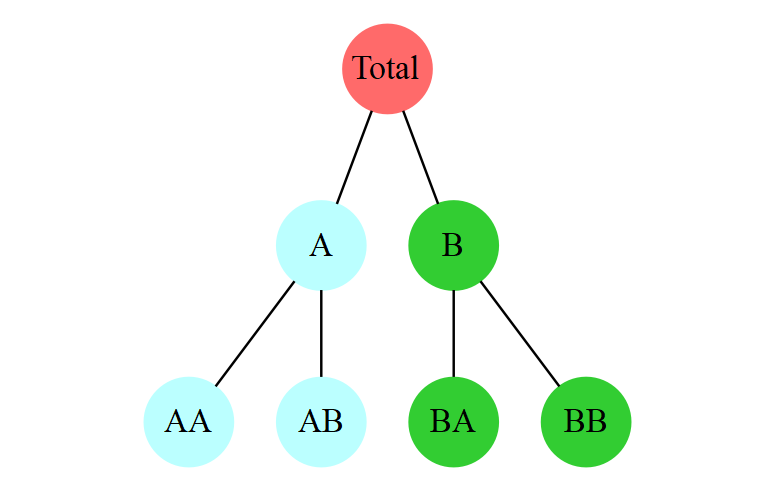
\includegraphics[width=0.4\linewidth]{Figures/treesimple}
	\caption{A two level hierarchical tree diagram}
	\label{fig:htstree}
\end{figure}

Large datasets often have a hierarchical structure (as seen in figure~\ref{fig:htstree}), in other words, data may organised into a tree-like structure, where broader categories with higher hierarchy may disaggregate into smaller categories with lower hierarchy. Vice versa, smaller categories with lower hierarchy may aggregate into broader categories with higher hierarchy. In a clinical trial, Adverse Events (AEs) caused by treatment drugs can be aggregate into body systems that are associated with AEs, thus creating a 2-level hierarchical structure. An example of a study considering such hierarchical structure is \cite{berry2004}, the study considers the probabilities of treatment drug cause an AEs and found significant differences in results between solo ( with each category independently modelled) and Hierarchical Bayesian Model (HBM) at the bottom level of the hierarchy, and suggested that the HBM could be a solution to the multiplicity problem found in large datasets. Similarly, disease diagnoses also have a complex, hierarchical structure, where different categories of diagnoses aggregated into broader categories. Standard such as International Statistical Classification of Diseases and Related Health Problems (ICD)\citep{WHO2019} are used to code for and organise disease diagnosis into a hierarchical structure. Information about ICD diagnoses often included in hospital archives for research and managerial purposes. Note that ICD diagnosis is not the equivalent to original diagnosis by doctors, descriptions of diagnoses can vary doctor to doctor, it is non-consistent and unorganised at first, this diagnosis is then classified into standard ICD diagnosis which is standard, organised and has clear hierarchical properties. 

%A hierarchical structure is also frequently seen in genetics data, Gene Ontology (GO) groups different genes into a multi-domain hierarchical network \citep{GO2007}, which is a representation of genetic relationship and network of significant GO categories often serve as a basis for genetic analyses.

\newpara 

We are interested in whether modelling the full hierarchy gives a better understanding of anomalies compares to modelling each category independently one level at a time. When modelling too broad a category, individual variations could be missed; when model too narrow a category, there may be too little data with non-significance. Vital information are likely be lost if we only consider one level at a time and if the information doe not situated at the level considered, so why not consider every possible level? A hierarchical model retains information from all level of the hierarchy and may provide better predictions compare to standard models that do not implicate the hierarchical structure of the data. The purpose of this research thesis is to investigate the use of Hierarchical Bayesian Models (HBM) as a possible approach for the detection of anomalies from hierarchical datasets. In this chapter, we describe examples of where these issues arise, and layout the technical background for our methods. 

%------------------------------------------------------------------------------------------

\section{Emergency Department Congestion}

While the world population continues to grow and age at an unprecedented rate, public healthcare system all over the world are expected to experience an increasing number of situations where a massive influx of patients overwhelms the current healthcare capability and in which congestion occur \citep{ morley2018emergency, wong2010understanding}. Other similar terms used to describe this situation include bottleneck and overcrowding. Congestion is shown to have negative influences on both patient and hospital staff, studies \citep{chambers2016burnout, khare2009adding, salway2017emergency} suggest that congestion is positively associated with adverse outcomes such as patient waiting time, short term patient mortality, medical errors, and professional burnout in hospital staff; therefore we would want to avoid or reduce the possibility of occurrence of congestions. Congestion seriously challenges the capability of public healthcare system worldwide and are becoming increasingly burdensome in many locations, and efforts from healthcare systems are struggling to kept pace with increasing demands. The overall consensus is that the demand from the ageing population is one of the major contributing factors to the current crisis, and the factor of ageing is unlikely to improve by time \citep{bayley2005financial, cornwall2004impact, wong2010understanding}. For instance, the national population projections by Stats New Zealand (2016) predicts a constant increasing trend in older (age 65 +) populations and show no sign of slowing down, so the problem of congestion in New Zealand in another hand, will most likely to correspond to this and worsen. 
%http://archive.stats.govt.nz/browse_for_stats/population/estimates_and_projections/NationalPopulationProjections_HOTP2016.aspx

\newpara

Shortage of staff for public healthcare services has been a prominent issue ever since a decade of decrease in the proportion of healthcare funding and deficit for the public health system in New Zealand \citep{akoorie2018, WB2019}. Due to limitations with medical material and human resources, hospital staff often had to operate at full capacity and are therefore under tremendous stress. Studies have shown that under-staffing is one of the key factors that contribute to the high prevalence of professional burnout in New Zealand’s public hospital senior medical workforce \citep{chambers2016burnout}. Described as “erosion of the soul” by Doctor Len Gabbard, in an article by \cite{HemOnc2008}, professional burnout is a term used in industry research that refers to a sense of emotional exhaustion, negative attitudes and sense of incompetence that often lead to reduced work effectiveness \citep{paterson2011professional}. Therefore burnout has negative impacts and to reduce this; we would need to optimise the way the hospital operates.  

\newpara

Due to the increasing patient influx and understaffing, some Emergency Department (ED) in the country struggled to cope with increasing patient arrivals; this is reflected from unacceptable delays before patients are admitted to hospital, transferred or sent home. Patient delay is a direct result of triage strategy \citep{MoH19triage} utilised by ED if congestion of patients occurs. When there is not enough staff to cope with patient demand, the patient at a higher triage is given a priority for treatment (higher the triage level, the more critical patient is believed to be). However, a critical flaw of the current strategy is that if congestion does not get resolved, and lots of patients require immediate treatment, a patient that is evaluated to be less urgent often gets delay after delay. In theory, a patient can be delayed for infinity if he is unfortunate enough, and the chance of further complication developing during the waiting period will only rise at every second of the clock ticking by. 

\newpara

A tragic case happened in New Zealand, back in 2015, where a woman in Wellington died after 12 hours of delay and ignorance in emergency medical service \citep{southland2015}. The news reported that \textit{“The emergency department was stretched by an influx of patient which lead to congestion and overcrowding”}, so ED staff had decided that the patient was not in an immediately life-threatening situation and decided to apply the triage strategy and therefore delayed medical service. What supposed to be a 30-minute delay had turned into more than an hour, and over the last 12 hour of the patient's life, ED staff failed to provide adequate monitor and care, which was believed to have contributed to the patient’s untimely demise.  It breaks your heart when you hear such case happening and you cannot stop wondering, what if the patient was treated in time? 

\section{Motivation}

Located at the start of the healthcare pathway \citep{MoH19pathway}, the Emergency Department (ED) and other forms of emergency health care are feeling tremendous pressure from increasing healthcare demands. Compare to primary healthcare, emergency healthcare is a 24/7 operating service characterised with unscheduled visits, and mostly deals with critical conditions that need immediate attention \citep{MoH19ed, MoH19primary}, therefore ED frequently encounters an influx of unanticipated emergencies such as major traffic accident, mass food poisoning and disease outbreaks. Unfortunately, due to limited and often diminishing resources, public healthcare facilities often had to operate at near full capacity to reduce operation costs \citep{salway2017emergency}, and this leaves a very small buffer zone to deal with abnormally high arrivals, so it is quite safe to suggest that ED staffs are underprepared for congestion.    

\newpara

The congestion crisis in the New Zealand healthcare service stood well recognised by the academic community, and there is a substantial amount of recent and ongoing research that aims at providing alternative operational strategies. For instance, \citet{adam2018} is currently working on simulations of Auckland city hospital’s Emergency Department with Pod model, where doctors form small cross-functional and multidisciplinary teams. Experimental trials had taken place at the Auckland city hospital during December 2018 - January 2019 to evaluate the effectiveness of Pods strategy compare to the precedent triage strategy. Another interesting study is a study by \citet{Cleland2018} that looked at developing algorithms to optimise staff rostering, compares to precedent; his algorithm found many new ways staff rostering can be improved and thus could improve the operational effectiveness of hospital. As we can see, we do have people approaching the problem in various ways. 

\newpara

For this thesis, we want to approach the problem of congestion in public hospitals through the perspective of Healthcare Logistics. As Prof.Dr. Stephan Nickle from Karlsruhe Institute of Technology (KIT) Quoted during the 2018 Operations Research Society of New Zealand (ORSNA) conference \citep{Nickle2018}, \textit{“Healthcare Logistics is all about the robustness and smoothness of the operation”}, what we want is stability and predictability of the operation, even if on paper we have a high efficiency, it is no good if this efficiency is often compromised. ED congestion often occurs during the periods of abnormal arrivals when the max capacity is overwhelmed; therefore, a success prediction/anticipation of such abnormal arrivals could provide valuable insight for operational planning and management. Public hospital was supposedly prepared, medical facilities continually being built, medical supplies prepared in advance, and staff were recruited base on predictions from historical mean arrivals. It would make sense to the thought that the public health system was well prepared, right? However, why are we still seeing congestions? Well, what happened is that the public health system had well prepared for normality, but has overlooked instances of abnormality. Lots of operational and logistics planning and based on mean values, however, means does not contain information about abnormality. To the inconvenience of everybody involved, congestion occurs during abnormal arrival events.

\newpara

If we could make sense of and make informed predictions about abnormal patient arrivals, it would provide helpfulness to the planning and management of the public healthcare system. Doctors can transfer, and medical supplies can be in preparation as soon as there is enough evidence suggesting an abnormal event is or will be happening. With better preparation and faster response to abnormal patient arrivals, the problem of congestion could be alleviated, and benefit both patient and healthcare staff. For patients, a shorter delay waiting period will increase the quality and timeliness of the medical service provided and reduce the risk of further complications during the wait. Moreover, for doctors, more preparedness should reduce professional burnout and increase efficiency \citep{chambers2016burnout, khare2009adding}. For this thesis, a strong emphasis is placed on modelling anomaly detection for patient arrivals, in the hopes of that extension on the understanding of anomalous arrival events could be made, and provide information for theoretical and real-life implications. 

%------------------------------------------------------------------------------------------

\section{Anomaly Detection} \label{chap:anom}

Anomaly detection refers to the field of studies of finding patterns in data that does not conform to the expectation, or that is out of normality. Studies of anomaly can trace back to the 19th century; an example is that in 1887, F. Y. Edgeworth a lecturer from King’s College, London wrote about what he termed as discordant observations, observations which \textit{“present the appearance of differencing in respect of their law of frequency from other observation with which they are combined”} \citep{edgeworth1887xli}. The term anomaly is quite similar to the term outlier, which is defined by “A data point that differs significantly from other observations” \citep{grubbs1969procedures}, and these two terms often used interchangeably. However, the term anomaly has a stronger contextual connection to the application side of the statistics, the wording itself literally meant, an event that is not of normal circumstance. 

\newpara

Anomaly detection found extensive application in fields such as cyber-security, finance, and healthcare. The reason why anomaly is catching so much research interest is that it often strongly associate with and directly translates into the occurrence of harmful situations and events in dynamic environments \citep{chandola2009anomaly, LaRosa2018}. The classic example of anomaly detection often described by Data scientists is the application of intrusion detection systems that are triggered by anomalies that are believed to be indicators of cyber-attacks. An indicator such as abnormally high website visits could be an indication of an HTTP POST attack, where the website processing capacity is overwhelmed, or maybe illegal data scraping, where private information is processed and exported from a website \citep{patcha2007overview, Target2018}. Due to growing concerns of potential bioterrorism attack following the anthrax letters attacks to various government officials during 2001, the US had been invested in the field of Biosurveillance in preparation for a potential bioterrorism attack \citep{grundmann2014current}. Therefore a substantial amount of research regarding population-level anomaly detection is available. For instance, back in 2003, \citep{wong2003bayesian} has presented the WSARE 3.0 algorithm, which stands for "What's Strange About Recent Events, version 3” for the detection of disease outbreaks in the US. Also, in \textit{Intelligence and Security Informatics: Biosurveillance}, a text published in 2007, \citet{bauer2007high} suggest the need of rapid data processing for anomaly detection to meet the increasing demand to disease surveillance at a population level. Their idea foreshadowed the recent rise in popularity of online streaming data systems that collect data from multiple sources continuously and provide statistical results right with each update.  

\newpara

For the case of patient arrivals, researchers often take an interest in time series data. That is, a continuing set of data that is recorded over specific time intervals \citep{das1994time}. If information about the time of each patient visit is available, it can be counted to give a time series data over time-periods, such as the number of patient arrivals per day. From the perspective of time series data, there are several important types of anomalies to be considered.  The first and most straightforward type is point anomalies, where a single time-period is anomalous. For example, traffic of a website may spike during a single night, when the website is under cyber-attack. The second and more complex type is period anomalies, where a continuing series of time-periods is anomalous. For example, the average daily spending during the Christmas period (let us say, the days between 1 December to 31 December) is expected to be much higher when compared to the average usual daily spending in other time frames. The last type, Contextual anomalies, where the occurrence of the anomalous time-period is believed to be context-specific. For example, the Admission rates for Emergency department patients may spike on any given day, when there is a mass injury event such as major car crashes \citep{chandola2009anomaly}. In this thesis, we want to focus on just the point anomaly, because other forms of anomalies are very context-specific and hard to perform in simulated settings. 

\newpara

There are many ways to decide whether a point or a pattern is abnormal and deviate from the expected; the most straightforward and often used approach is to set up value as thresholds, and then anomalies can be detected simply by raising alarms for observing values beyond the threshold (figure~\ref{fig:anomaly}).

\begin{figure}[h]
	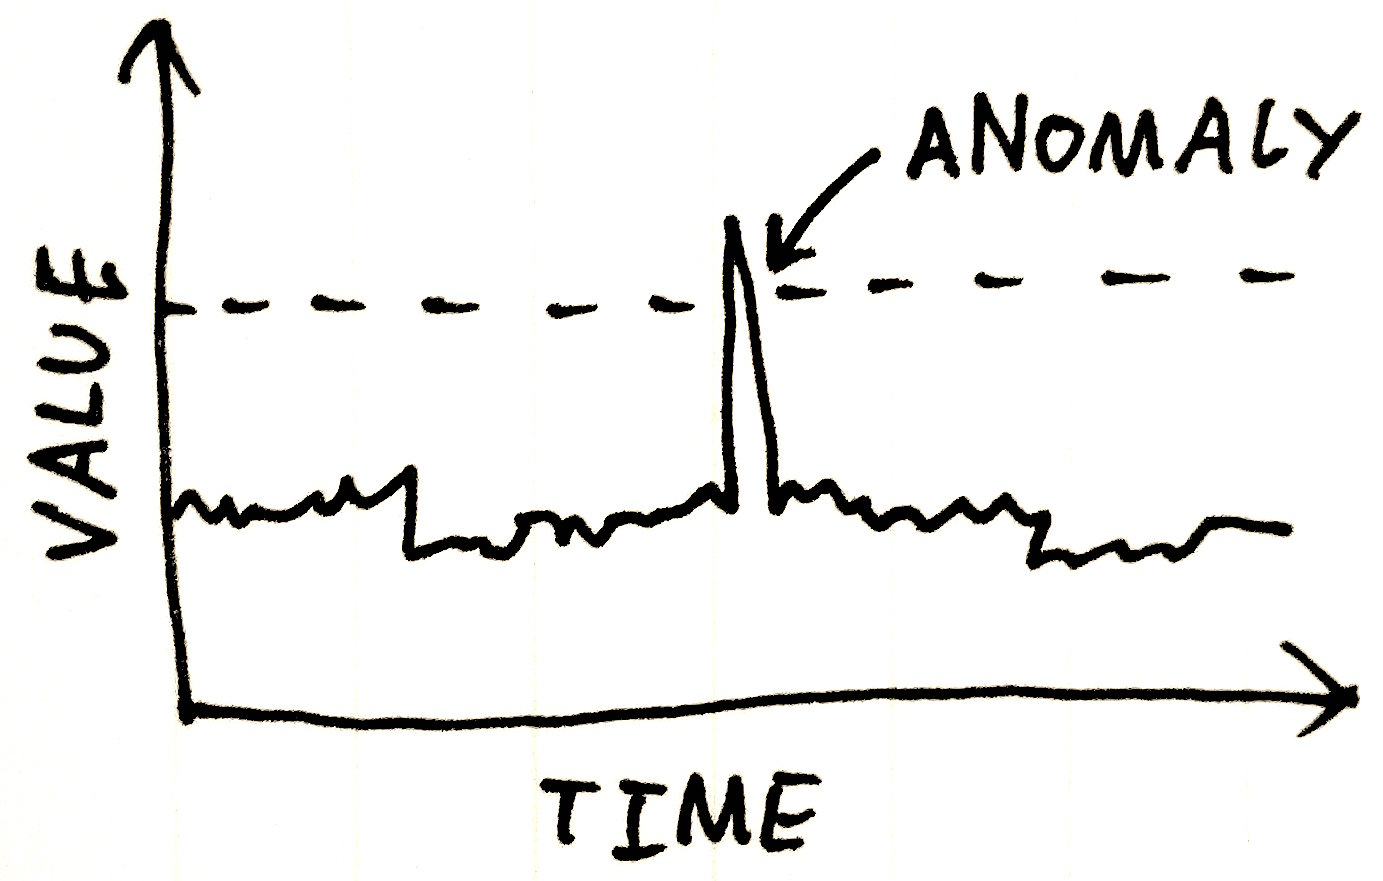
\includegraphics[width=47mm]{Figures/external/simple_anomaly}
	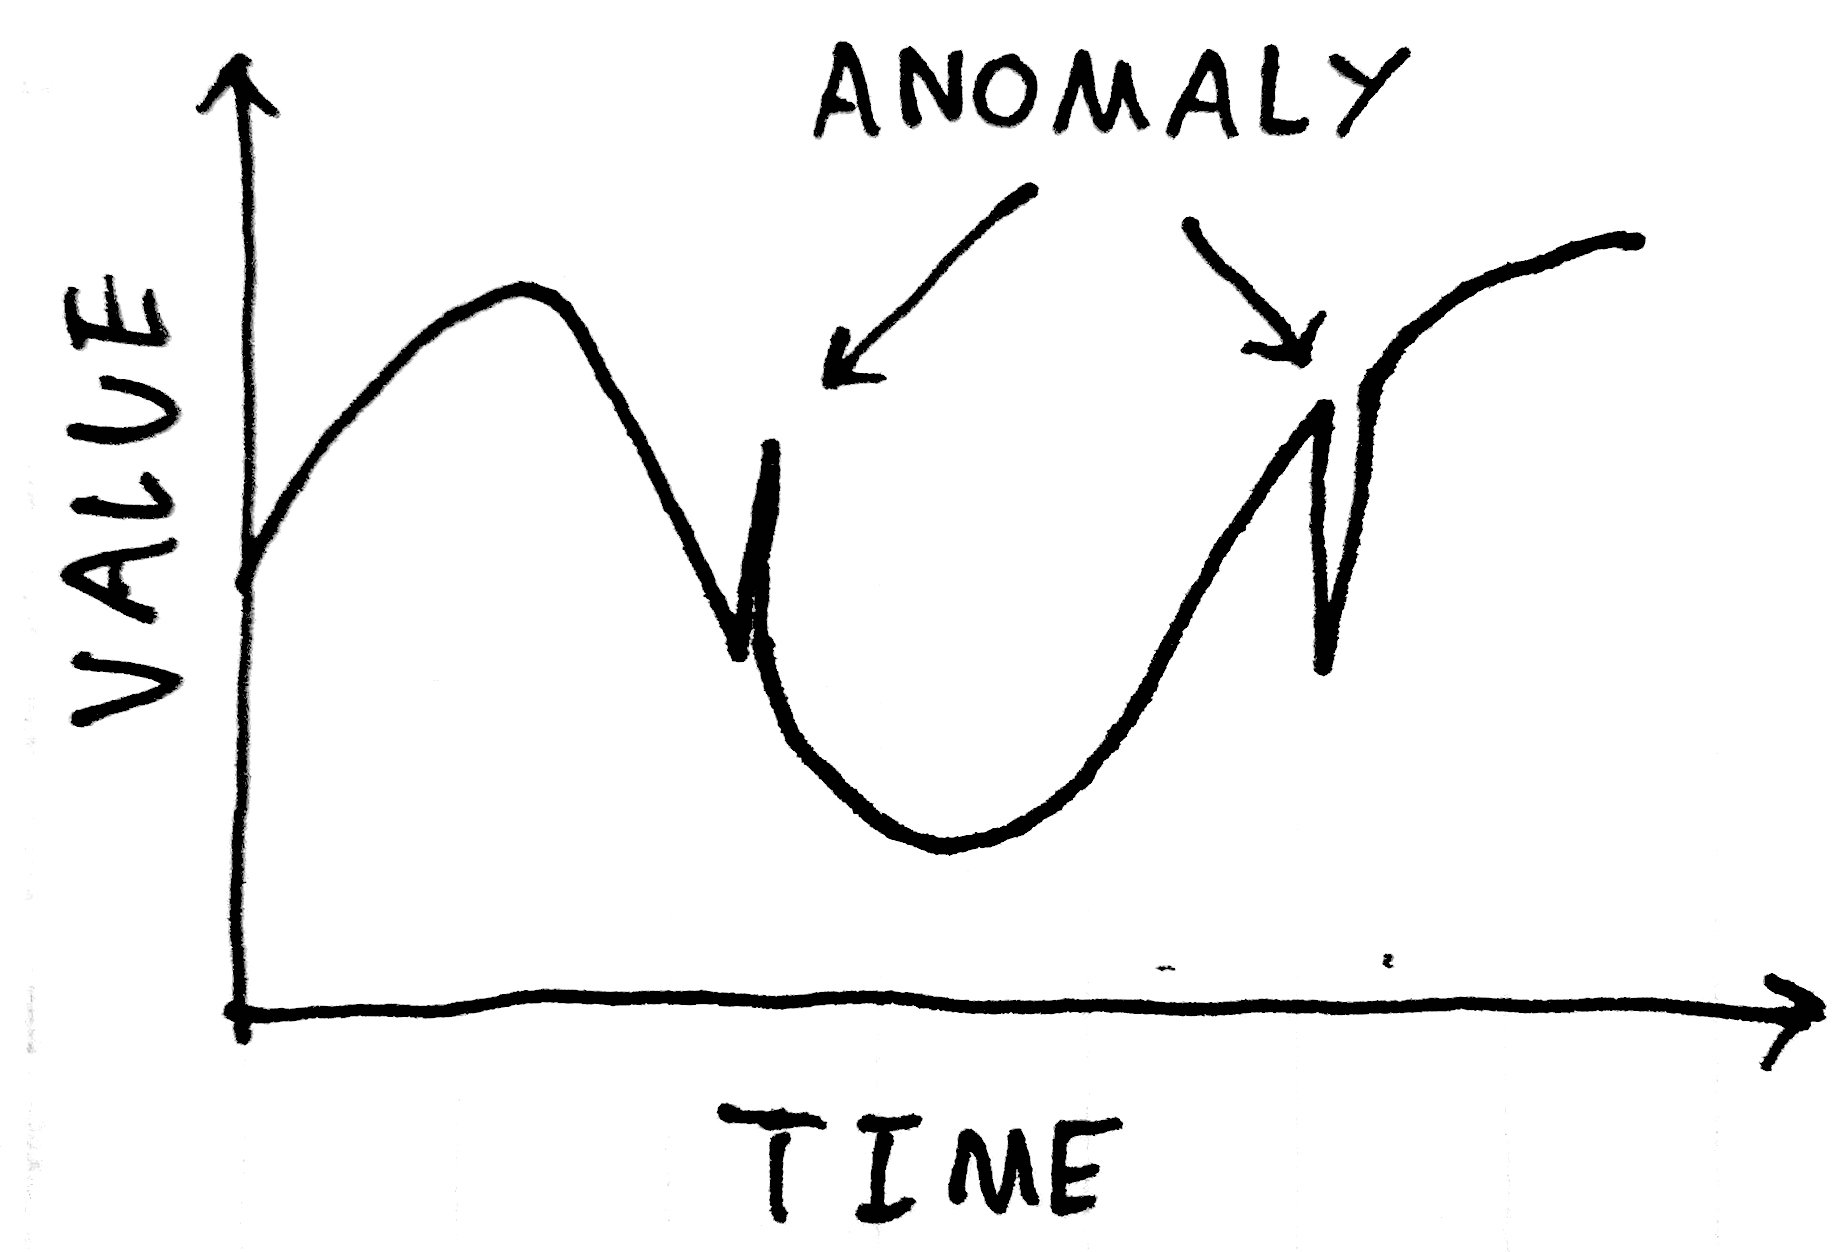
\includegraphics[width=47mm]{Figures/external/harder_anomaly}
	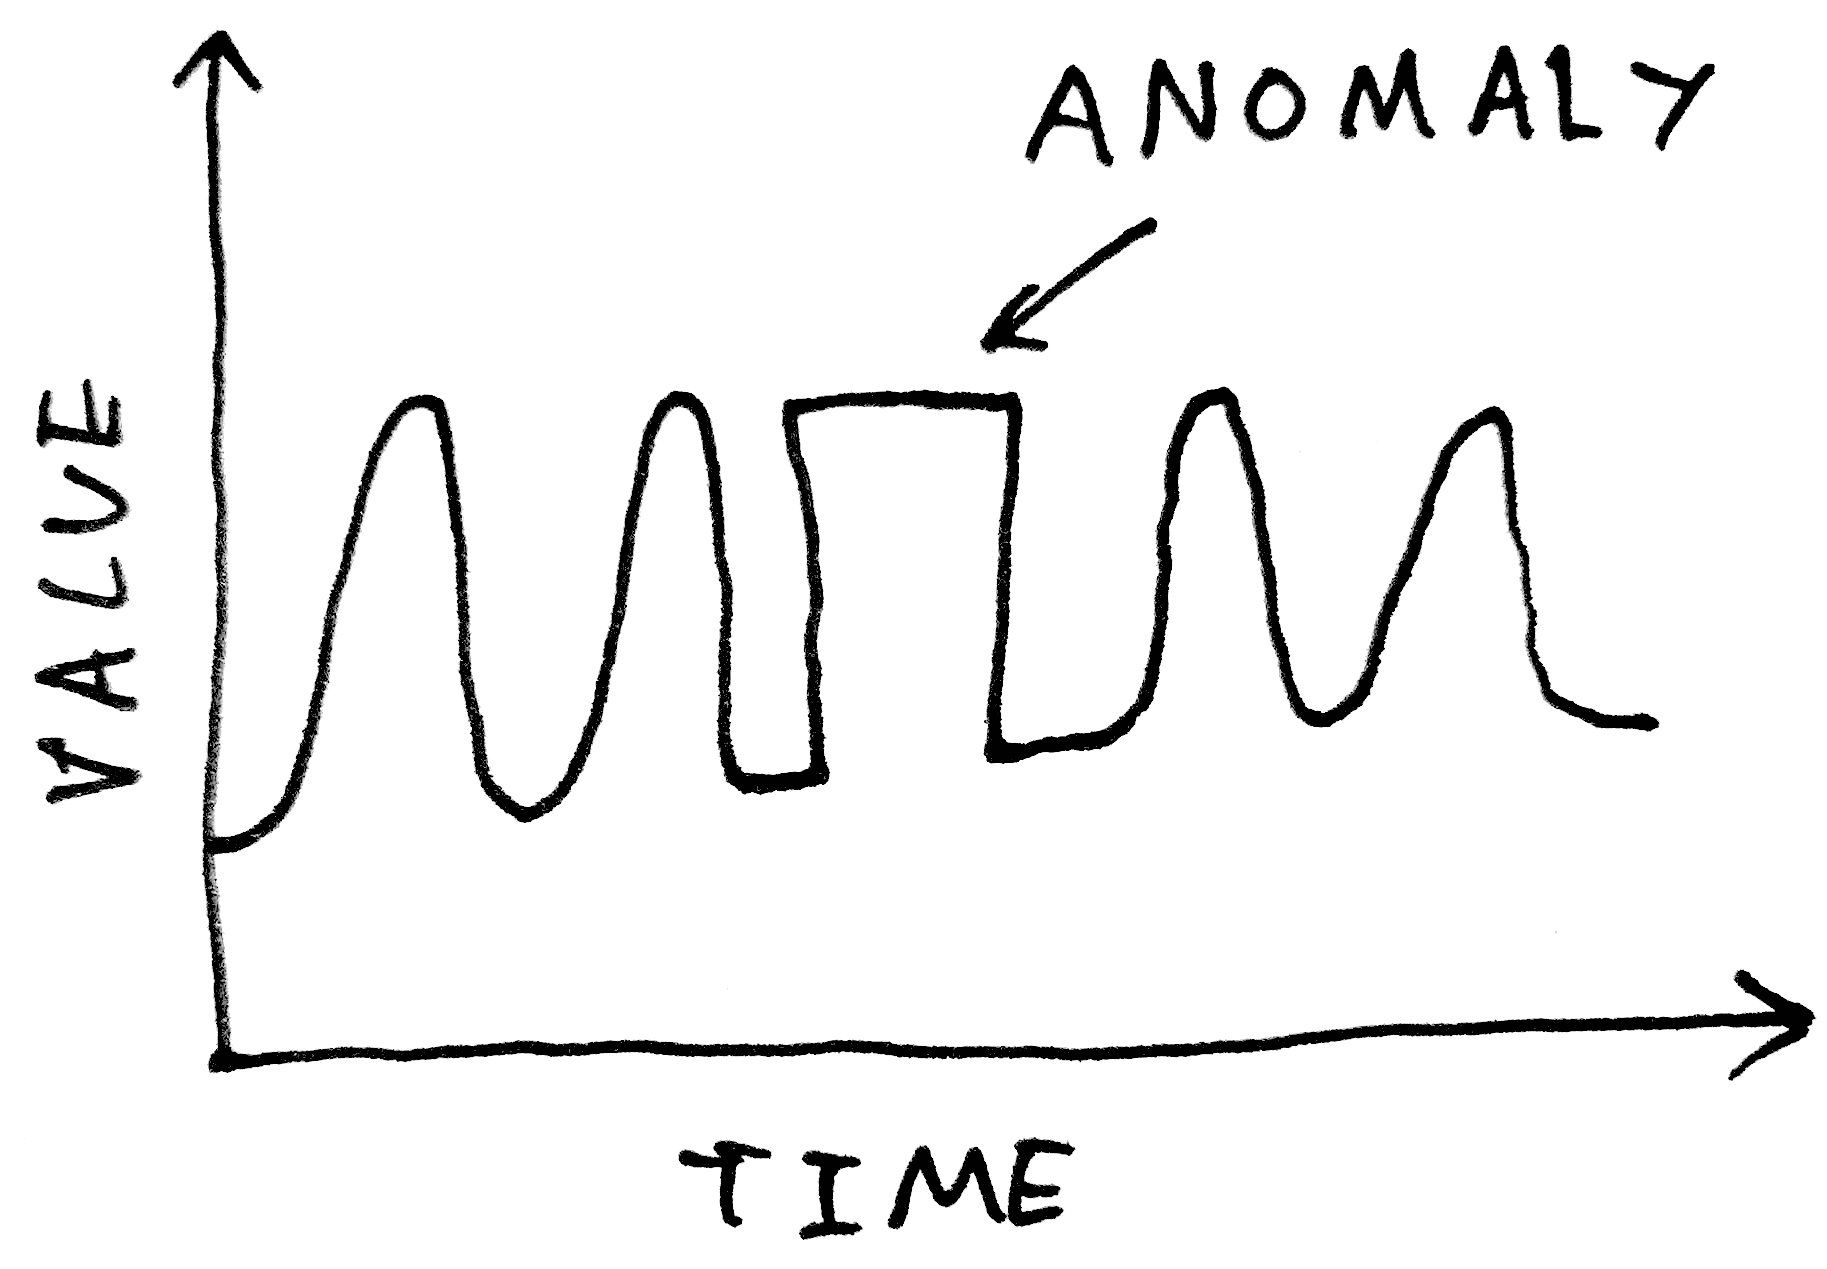
\includegraphics[width=47mm]{Figures/external/really_hard_anomaly}
	\caption{Anomaly Visualisation from \citet{Rahtz2015}}
	\label{fig:anomaly}
\end{figure}

\citet{wong2003bayesian} considered the threshold approach and proposed the standard algorithm. Their anomaly detector considers the mean $\mu$ and variance $\sigma$of the total number of records on each day, and used algorithm shown in equation~\ref{equ:threshold} to calculate a threshold, For the algorithm $\Phi^{-1}$ is the inverse to the cumulative distribution function of a standard normal with an user-defined p-value. If the aggregate daily counts of health care data exceed this threshold during the evaluation period, an alarm can raise. 

\begin{equation}\label{equ:threshold}
\begin{aligned}
threshold = \mu + \sigma * \Phi^{-1}(1-\dfrac{\text{p-value}}{2})
\end{aligned}
\end{equation}


We propose a simpler algorithm that approaches the threshold set up from a more practical point of view, rather than a theoretical statistical value such as $\Phi^{-1}$ used by \citet{wong2003bayesian}. We want to create two values called load ($\mu$) and capacity ($C$), $C$ are the full treatment capacity in terms of absolute value of a department, and $\mu$ the average number of capacity being occupied and utilised. In theory, $\mu$ and $C$ could be generated from hospital records such as the number of hospital beds occupied, the number of doctors that are currently treating a patient and not available for another patient in a short notice, and any other available measures of hospital operational capacities. $\mu$ over $C$ gives a load fraction, which are referred as capacity in terms of percentage. If we assume that the healthcare system is expected to be operating at a capacity value ($k$) of 0.8, it would mean that on average, 80\% of total possible treatment resource during a specific period is utilised. 

\begin{equation}\label{equ:threshold2}
\begin{aligned}
k = \mu C^{-1}
\end{aligned}
\end{equation}

In simple terms threshold would just be the full capacity $C$, however we want to compare between low and high capacity departments so capacity $k$ are used in our study. So if a hospital department on average treats 100 patient per day, and this department is considered to be operate at 80\% capacity, the threshold would be $100 \times 0.8^{-1} = 100 \times 1.25 = 125$. The idea is that when we reached the threshold, it would mean that the healthcare capacity of the period had reached 100\%, and there is no more capacity for more patients, and in theory, this is when congestion would for definitely, occur. Instead of only considering operating cost, an ideal operating percentage should be relatively high to reduce operating cost, and have gives a low chance of overcapacity due to the anomalous event. Following up on the idea by Stephan Nickle, mentioned in the previous section, we propose that increasing the operational capacity without considering anomalous events could jeopardise the smoothness of operation, and cause even more loss of operating efficiency due to increased probability congestions. 

\newpara

To create an alarm system that raises alarms for hospital congestion, we could apply a threshold on to patient arrivals, with every increase in the number of patients arrived, it would become more likely that a threshold can exceed. However, the catch is that we should also incorporate external information such as the number of bed available instead of only considering with numerical probability. How could we possibly know if we have reached the full hospital capacity if we only consider the number of beds used, without knowledge of the number of total beds available? With only information about observed arrivals, we could work out the likelihood of observing specific arrival numbers, but this outcome does not make any practical sense by itself. Information is one of the reasons why the standard algorithm proposed by \citet{wong2003bayesian} although performed excellently, still seem weak for practical applications. The standard algorithm considers the threshold as the im-probability from the data structure and does not consider what determines the threshold, the ability or the capacity for hospitals to treat patients. A particular statistical inference approach does incorporate external information and solves this problem, as people might have guessed already, Bayes. 


%------------------------------------------------------------------------------------------
\section{Hierarchical Bayesian Models}
\subsection{The history of Bayesian statistics}

The term Bayesian refers to a range of statistical techniques that approach statistical inference. The term Bayesian makes tributes to the 18th-century mathematician, the late Reverend Thomas Bayes (1702-1751) \citep{stigler2002statistics}. Bayes theory was published after Bayes's death and was pioneered and popularised by the much-acclaimed Mathematician Pierre-Simon Laplace (1749-1827) in his 1814 "Philosophical essay on probabilities" \citep{mcgrayne2011theory}. The theorem was non-popular at first as statistical solutions were often impossible to obtain, apart from conjugate distributions [ref pg 493 of stats 732 note], which refers to solutions in the same algebraic form of prior with alteration in parameters. The development of Markov chain Monte Carlo (MCMC) techniques in 1940 and generalisation of personal computing device provided the solution to the fatal flaw, application of Bayesian methods was seen since 1990 and is now becoming ever popular and poses a severe challenge to the classical frequentist approach to statistical inference \citep{allenby2005hierarchical, mcgrayne2011theory}.

\subsection{Bayesian inference}
\begin{displayquote}
	\textit{How do you tell if a statistician is a true Bayesian?} \\
	\textit{Ask them what time it is.} \\
	\textit{If they tell you the time, they’re a frequentist;}\\
	\textit{A Bayesian will ask “What time do you think it is?".} \\
	
	\hskip 5cm --- Geoff \citet{Johns2018}
\end{displayquote}

The Bayesian approach to statistical inference is a form of evidential probability, where repeatable observations serve as evidence in the determination of probability characteristics of certain events \citep{paulos2011mathematics,wheeler2011evidential}. The principle is, given information of past event as prior probability  and taken into account current evidence as likelihood, Bayesian are able to update and deduce the posterior probability, an evidence based proposition \citep{laplace1998pierre}. The essence of Bayesian inference lies within the Bayes' theorem (alternatively Bayes' law, Bayes' rule)\citep{brewer13}, it can summarised mathematically as the following equation:

\begin{equation}\label{baye1}
\begin{aligned}
\underbrace{\Pr(A | B)}_{\text{posterior}} &= \frac{\overbrace{\Pr(B | A)}^{\text{likelihood}} \overbrace{\Pr(A)}^{\text{prior}}}{\underbrace{\Pr(B)}_{\text{marginal likelihood}}}
\end{aligned}
\end{equation}

Given two events $A$ and $B$,
$\Pr(A|B)$ is the conditional likelihood of event A occurring given that  B is true, which represents the posterior. 
$\Pr(B|A)$ is the conditional likelihood of event B occurring given that  A is true, and this represents the likelihood. 
$\Pr(A)$ and $\Pr(B)$ are the probabilities of observing  A and  B independently of each other; this is the marginal likelihoods. $\Pr(A)$ represents the prior, and $\Pr(B)$ is a measure of evidence, without conditioning on prior.In other words,  A here is a parameter of interest and B is a set of observations that are informative about A. 

\newpara

In probability statistics, the characteristic of a statistical population or a statistical model can be quantified with a number of parameters, often noted as $\theta$ the parameter vector, where $\theta = \{\theta_i ,...,\theta_p\}$, and p  the length of the parameter $\theta$. For example, the parameter $\lambda$ characterised a Poisson distribution, where $\lambda$ can be interpreted as the average number of events per interval. The probability distribution function of Poisson can be given an equation with the parameter $\lambda$ and a vector of observed data as:

\begin{equation} \label{baye2}
\begin{aligned}
P\left( x \right) &= \frac{{e^{ - \lambda } \lambda ^x }}{{x!}}.
\end{aligned}
\end{equation}

If we consider $\Theta$ as our parameter and $X$ as our observations, in terms of the generalised distribution function, Bayes theorem can express as

\begin{equation} \label{baye3}
\begin{aligned}
f_{\Theta|X}(\theta|x) 
&= \frac{f_{X|\Theta}(x,\theta)}{f_X(x)} \\
&= \frac{f_{X|\Theta}(x|\theta) f_\Theta(\theta)}{f_X(x)} 
\end{aligned}
\end{equation}

For equation \ref{baye3} $f_{\Theta|X}(\theta|x)$ is the posterior density, $f_{X|\Theta}(x,\theta)$ is the joint density of $x$ and $\Theta$, which can be transformed into conditional density $f_{X|\Theta}(x|\theta)$ and marginal density $f_\Theta(\theta)$, lastly we have the marginal density of $f_X(x)$.


\begin{equation} \label{baye4}
\begin{aligned}
f_{\Theta|X}(\theta|x) 
&= \frac{f_{X|\Theta}(x|\theta) f_\Theta(\theta)}{f_X(x)} \\
&= \frac{f_{X|\Theta}(x|\theta) f_\Theta(\theta)}{\int f_{X|\Theta}(x|\theta) f_\Theta(\theta) d\theta } \\
&\propto \frac{L(\theta) f_\Theta(\theta)}{c}\\
\Pr(\theta|x) 
&\propto \Pr(x|\theta)\Pr(\theta)\\
\textbf{\text{Posterior}} 
&\propto \textbf{\text{Likelihood}} \times \textbf{\text{Prior}}
\end{aligned}
\end{equation}

If we consider the case of continuous distributions in equation \ref{baye4}, $f_X(x)$ is the distribution of X, which can be expressed as integral $\int f_{X|\Theta}(x|\theta) f_\Theta(\theta) dx$ and we know it is a constant ($c$) with respect to $\theta$. $f_{X|\Theta}(x|\theta)$ also correspond to the Likelihood function $L(\theta)$ as a function of $\theta$. After these transformation we see the proportional property of $f_{X|\Theta}(x|\theta)$ ,$L(\theta)$ and $f_\Theta(\theta)$. We can derive the conclusion that posterior probability distribution of the parameter of interest is proportional to the product of prior probability distribution and observed evidence, and the posterior is an adequate estimation that reflects the probability characteristics of certain event or distributions \citep{Wong19}. Overall, this is the theorem behind Bayesian inference, given prior and likelihood, we can deduce the posterior. 

\subsection{Simulation-based estimation}

As we had mentioned in the previous section, in Bayesian statistics, the posterior distribution can be manually calculated to obtain conjugate solutions. The basic idea is that a standard distribution can work as the approximation of prior distribution, and with certain likelihood functions a posterior distribution with a distribution from the same family can be formed, and this made it possible to derive solutions as going from prior to posterior distribution is simply a matter of figuring out how the parameter of the distribution had changed. \citep{Wong19}. For example, a $Beta(\alpha,\beta)$ prior can be multiplied with a $Binomial(n,x)$ likelihood to form a $Beta(\alpha + x,\beta+n - x)$ posterior distribution with some mathematical manipulations, shown here in equation \ref{baye5}. 

\begin{equation} \label{baye5}
\begin{aligned}
& \frac{\Gamma(\alpha+\beta)}{\Gamma(\alpha)\Gamma(\beta)}\theta^{\alpha-1}(1-\theta)^{\beta-1} \times {n \choose x}\theta^x(1-\theta)^{n-x}\\
=& \text{Constant}\times\theta^{\alpha+x-1}(1-\theta)^{\beta+n-x-1}
\end{aligned}
\end{equation}

However, for cases with non-conjugate prior distribution, it is challenging to perform mathematical calculations; therefore, alternative methods are often used to calculate the characteristics of the posterior distributions. A way to calculate the posterior distribution is to approach with a simulation-based estimation method, for which multiple generations of repeated samples can be used to converge into a reasonably estimation \citep{congdon2007bayesian}. Markov chain Monte Carlo (MCMC) methods are often utilised by Bayesian to obtain repeated samples from a probability distribution, the idea of a Markov chain is that the probability characteristics of each draw depend only on the state in the previous event \citep{Fewster14}. We could represent the Markov property in mathematical notation as following equation \ref{baye6}, where a sample from time $t+1$ only depends on a sample from time $t$ and all previous observation does not matter.

\begin{equation} \label{baye6}
\begin{aligned}
\Pr(X_{t+1}|X_t,...,X_0)
&= \Pr(X_{t+1}|X_t)
\end{aligned}
\end{equation}

The Metropolis-Hastings algorithm is a family of MCMC methods useful for sampling from probability distributions from which direct sampling was not possible. [Hastings, 1970]. The Gibbs sampling is a particular case of the Metropolis-Hastings algorithm often used in Bayesian statistics to obtain a sequence of sample observations which are approximately from a specified multivariate probability distribution, this sequences of sample observations will eventually converge and form a stationary Markov chain, that are often inferred as posterior distribution. The basic idea of Gibbs sampling is to repeatedly sample from the conditional distribution of one variable of the target distribution, given all other variables (full conditional distribution). In other words we are updating our parameter one at the time as individual iterations, while considering current value of the other parameters. 

Just Another Gibbs Sampler (JAGS) is a program designated for the analysis of Bayesian models using MCMC simulation \citep{plummer2003jags}. JAGS can work within the R language and environment, with the use of \texttt{rjags} \citep{rjags} and or \texttt{R2jags} \citep{R2jags} package from the Comprehensive R Archive Network (CRAN), using the statistical software, R \citep{R}. Details about download and installation of JAGS and R is in official websites, and examples of a JAGS script used to simulate results used for this thesis is presented in the Appendix.

\subsection{Bayesian against Frequentist}

There are two significant approaches to statistical inference, the frequentist approach, and the Bayesian approach. The frequentist school place emphasises on the sampling distribution of the observed data, Frequentist treats observations as a random experiment with fixed parameters across random samples and aims to calculates the im-probability of obtaining an observed result. By contrast, the Bayesian school base their inference on Bayes formula (equation~\ref{baye1}), Bayesian treat observations to be fixed and assume randomness for model parameters, and aims to update prior into posterior. Thus a significant difference between frequentist and Bayesian is that they give a different interpretation of results, as shown in figure~\ref{fig:freqbaye}, frequentist often give a p-value where Bayesian often present posterior probability. Each approach has its strength and weaknesses. However, the Bayesian approach seems to be a more suitable option for our analysis in many ways.

\begin{figure}[!h]
	\centering
	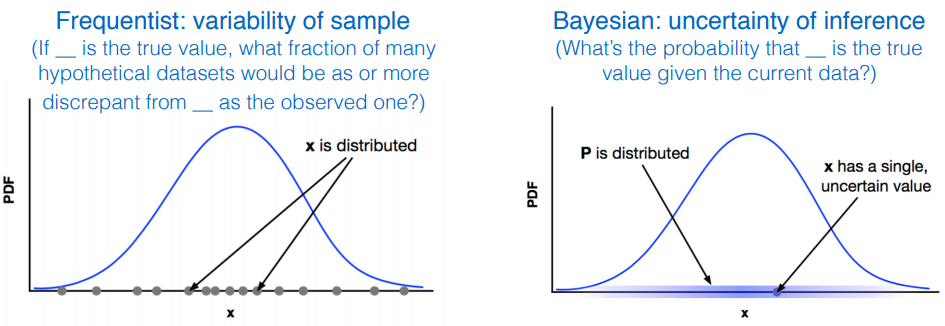
\includegraphics[width=0.7\linewidth]{Figures/freqbaye}
	\caption{Visualised comparison of frequentist and Bayesian results, from \citet{Wolfgang2016} }
	\label{fig:freqbaye}
\end{figure}

A significant problem of the frequentist approach is that its interpretation of result inevitably encourage people to fixate on numerical determinants such as p-value and did not allow for uncertainty. Study such as \citet{open2015estimating} have shown that psychology experiments with frequentist results often have weaker claim to evidence than evidence suggested by p-value from studies, a large proportion of the studies are not repeatable. A p-value of 0.051 and a p-value 0.049 are very similar probability-wise; however, people could deduce significance and non-significance just because 0.049 is lower than the significance level, and 0.051 is not if they fixate on the significance level of 0.05.  Results from Bayesian analyses are less prone to such issue, as it results are in posterior probability distributions, even though a it is harder to interpret, it contains much more information within the posterior probability distribution compares to the frequentist p-values. Secondly, Bayesian inference allows the inclusion of external information from sources other than just the observation; this is a form of evidential probability and allows for sequential learning \citep{baath2015, Jia2018}. For time-series data, the way Bayesian includes information from both the past and present make much more sense than considering only the present observation because datasets with sequential measurements such as time-series data often observe autocorrelation, where information from the past strongly associates with present observations. Also, as mentioned in the previous section, incorporating external information about hospital capacity makes much more sense than the frequentist approach as the primary determining factor for hospital congestion are the capacity it could accommodate. We could observe a very improbable arrival, but if this number still falls under the capacity, there is no congestion. Lastly, Bayesian has an advantage over frequentist for large datasets with complex structures. As models get more complex and more nested, the likelihood for over-fitting, over-parametrisation and multiplicity often increase for simple frequentist models. Bayesian allows utilisations of finer definitions for highly custom models that also penalises over-parametrisation \citep{baath2015, bolker2009generalized, kruschke2015bayesian}.

\subsection{Prior Selection}

The essence of Bayesian inference lies within the Bayes theorem, that is, given prior and likelihood, we can deduce the posterior. A prior probability distribution refers to a probability distribution that expresses ones' prior beliefs about an observation. For example, the prior could be the probability distribution representing the expected patient arrivals at an Emergency Department (ED). There are several acceptable methods of obtaining the prior. Firstly, prior can be determined from past information, such as historical hospital records. Secondly a prior can be a purely subjective opinion from an expert in the field, an ED staff making claims about average patient arrivals also seem reasonable, and lastly statistical principles can be applied to synthesis a prior, a normal distribution is often used for large samples if the prior belief if that the unknown parameter is most likely equal and have few outliers. Also, people often choose to use a conjugate prior to simplifying the calculations of the posterior distribution.

\newpara

Priors can be classified by the amount of information it contains, in terms of informative, weakly informative and non-informative priors. Informative priors define specific information about a variable. Historical information about patient arrivals can be modelled to give predictions, and optimum solutions can be used as the prior. A weakly informative prior contains partial information about a variable, parameters are more vague and rounded but still regularises the parameter estimates reasonably well. A possible standard to distinguish informative and weakly informative prior is that for informative priors, people with different backgrounds are likely to have very different idea about the prior, and for weakly-informative prior, people from different background should agree with the prior. Non-informative priors in another hand, contains no information, such as the use of a uniform or flat line distribution that contain no variation. Informative priors are the proper way to introduce the available informations to the model, and will provide solutions to computational issues and improve efficiency if it was correctly assigned, non informative prior in other hand challenges the notion of prior, but are often thought of as the reference models,and serve as starting point of more informative prior distributions. The weakly informative prior stands as a compromise between two sides \citep{carlin2008bayesian, golchi2016informative}.

\newpara

Parameters of prior distributions are also the hyper-prior because it gives rise to the parameter being estimated. For example, if parameter $\lambda$ of a Poisson distribution is used to model the parameter $\mu$ of a normal distribution, it is then said that $\lambda$ is a hyper-parameter. Hyper-parameters themselves may have hyper-hyper-prior distributions expressing beliefs about their values. Moreover, a Bayesian model with more one level of priors is called a hierarchical Bayesian model.

\subsection{Hierarchical Bayesian models}

\begin{figure}[hb]
	\centering
	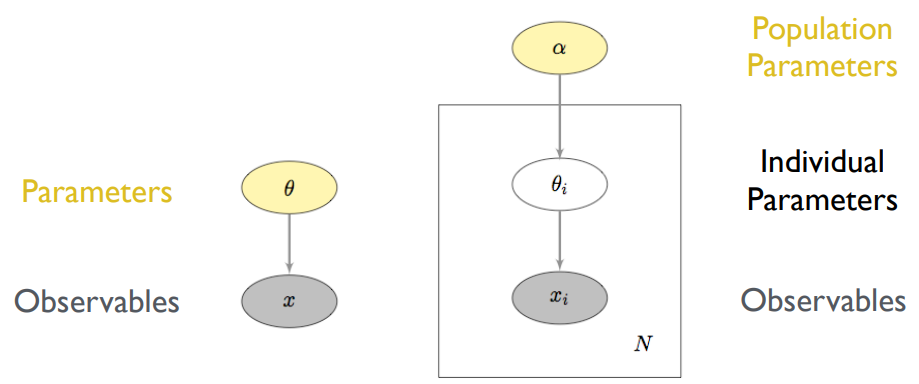
\includegraphics[width=0.7\linewidth]{Figures/hbm}
	\caption{Modelling structure between regular and Hierarchical Bayesian Models, from \citet{Wolfgang2016}}
	\label{fig:hbm}
\end{figure}

Information about the structure of hierarchical data can be processed and utilised with the use of Hierarchical Bayesian Models (HBM). Parameters within the HBMs contain a nested hierarchical structure, which meant that parameters of a higher hierarchy control the parameters of the lower hierarchy. The left plot in figure~\ref{fig:hbm} described the relationship between parameters and observations of an Independent Bayesian Model (IBM), for the case of IBM, observations are directly generated from parameters from a single level probability distributions and thus considered independent. The right plot in figure~\ref{fig:hbm} described the relationship between parameters and observations of an HBM, for the case of HBM, population parameters and observations control individual parameters is generated from a multi-level probability distributions \citep{gelman2007data, Wolfgang2016}, therefore we have this pooling of information, and there is no independence.

\newpara

In Bayesian terms, a simple IBM follows equation~\ref{baye8}, considering only the individual parameter $\theta$ and observations $x$. For an HBM extra population parameter, $\alpha$ can be incorporated and written with the formula shown in equation~\ref{baye9}. 

\begin{equation}\label{baye8}
\begin{aligned}
\overbrace {p(\theta|x)}^{\text{Posterior}} & \propto \overbrace {p(x|\theta)}^{\text{Likelihood}} \overbrace {p(\theta)}^{\text{Prior}} 
\end{aligned}
\end{equation}

\begin{equation}\label{baye9}
\begin{aligned}
\overbrace {p(\alpha,\theta|x)}^{\text{Posterior}} & \propto \overbrace {p(x|\theta,\alpha)p(\theta|\alpha)}^{\text{Likelihood}} \overbrace {p(\alpha)}^{\text{Prior}}
\end{aligned}
\end{equation}

\newpara

for level 1 categories i and level 2 categories $j \in i$, 

\begin{equation}\label{baye9}
\begin{aligned}
x_{ij}|\theta_{ij}&\overset{ind}{\sim}f(.|\theta_{ij})\\
\theta_{ij}|\alpha&\overset{iid}{\sim}f(\alpha)\\
\alpha&\sim f(.)
\end{aligned}
\end{equation}

where $i = 1,...,n,$ and $j = 1,...,n_i,$ and

\begin{equation}\label{baye9}
\begin{aligned}
x_{ij}|\theta_{ij}&\overset{ind}{\sim}f(.|\theta_{ij})\\
\theta_{ij}|\phi_i&\overset{iid}{\sim}f(\theta_{ij}|\phi_i)\\
\phi_i|\alpha&\overset{iid}{\sim}f(\phi_i|\alpha)\\
\alpha&\sim f(.)
\end{aligned}
\end{equation}

The former model is the ‘independence’ model (no pooling), and the latter is the ‘hierarchical’ model (pooling within level 2). 

\newpara

The way HBMs integrate group information with a pooling process is a partial-pooling model that compromise between complete-pooling and no-pooling models. With complete pooling, each unit is assumed to have the same parameter, leaving no independence and therefore contain zero population variance. With no pooling, each unit is assumed to have different and independent parameters, and this complete independence corresponds to infinite population variance. Both complete-pooling and no-pooling models have significant applications in preliminary statistical analyses but unlikely to accommodate real-life data very well; as it is unlikely and does not make sense for scenarios of no independence and complete independence to happen in real-life. For HBMs, individual estimates tend to shrink toward the population mean, and this effectively lowers the overall Root Mean Square Error (RMSE). RMSE is a popular goodness-of-fit value used to measure the difference between real and predicted values during cross-validation analyses. Therefore, there is no surprise that studies have shown that hierarchical models tend to give a better prediction compare to no-pooling and complete-pooling models in all levels \citep{gelman2006multilevel, gelman2007data, park2004bayesian}. 

\subsection{DIC}

In Bayesian statistics, deviance is often used to evaluates the goodness-of-fit statistic for a model. \citet{spiegelhalter2002bayesian} has proposed the idea of using deviance information criterion (DIC) as a tool for goodness-of-fit comparison between Bayesian models. DIC is defined as the expected deviance $\bar{D}$ plus the effective number of parameters in the model $p_D$. 

\begin{equation} \label{DIC}
\begin{aligned}
DIC = \bar{D}+p_D 
\end{aligned}
\end{equation}

which is also equivalent to 

\begin{equation} \label{DIC2}
\begin{aligned}
DIC = D(\bar{\theta}) +2p_D
\end{aligned}
\end{equation}

 where $\bar{\theta}$ is the expectation of $\theta$.
 
 \newpara
 
 DIC can be thought of as an approximation to the deviance, or the out-of-sample predictive error, therefore models with lower DIC are preferable.DIC criterion is particularly useful in Bayesian model selection problems where the posterior distributions of the models have been obtained by Markov chain Monte Carlo (MCMC) simulation. The smaller the DIC, the more accurate the model is for predictions and thus preferred. Model DICs can be generated by using \texttt{dic.samples} function from the \texttt{rjags} package within the R environment, The definition of $p_D$ used by \texttt{dic.samples} function is the one proposed by Plummer (2002).

\subsection{Effective Sample Size}

The idea effective sample size (ESS) is to provide a unit that converts dependent samples into units of independent samples. In other words, the ESS is an estimate of the sample size required to achieve the same level of precision if that sample was a simple random sample. For the case of highly correlated samples, 1,000 samples from a Markov chain can be only equivalent to 100 independent samples. In the case of a weakly correlated sample, 1000 samples from a Markov chain can be only equivalent to 300 independent samples \citep{Cook17, kass1998markov}. The equation for ESS is:

\begin{equation} \label{ESS2}
\begin{aligned}
\mbox{ESS} = \frac{n}{1 + 2\sum_{k=1}^\infty \rho(k)}
\end{aligned}
\end{equation}

Where n is the number of samples and $\rho(k)$ is the correlation at lag $k$.The MCMC process causes the draws to be correlated, as shown in the Markov chain algorithm (equation~\ref{baye6}) the sample from time $t + 1$ depends on the sample from time $t$. This means that the effective sample size is generally lower than the number of draws and is used for calculations. Any Markov chain between 0 ESS and completely ESS is reasonable.

%------------------------------------------------------------------------------------------    

\section{Hierarchical time-series}

\subsection{ Structure of Hierarchical time-series}

A time series refers to a series of data points that are ordered in time and or contain information about when the numbers were recorded \citep{das1994time,hyndman2018forecasting}. Time series analysis is an intriguing part of epidemiology and clinical research because time often has a strong association with the development of diseases and often reflect essential population-level information. Time series in epidemiology and clinical research often can have a hierarchical structure, where many time-series aggregate together to form broader categories of time series by specific population attributes.  Finer International Statistical Classification of Diseases and Related Health Problems (ICD)\citep{WHO2019} categories at a lower level of hierarchy diagnoses can be aggregated into broader categories at a higher hierarchy level. 

\newpara

A hierarchical time series (some time called grouped time series) can be represented with a hierarchical tree diagram. Figure~\ref{fig:treesimple} shows a simple 2 level hierarchical structure. At the very top of the hierarchy, it is the total; it can be calculated by summing of all categories, it represents the sampling population, and can be thought of as the start (level 0) of the hierarchy. The total can be disaggregated into subcategories at level 1 of the hierarchy, and subcategories can be disaggregated into sub-subcategories at level 2 of the hierarchy, and so on. Categories a hierarchy higher can be thought as the parent, and categories a hierarchy lower can be thought as the children of another hierarchy. The observations of the total series given time $t$ is denoted by $y_{total,t}$ for $t=1,2,3…,n$ with $,t$ standing for given time $t$ and $n$ standing for the length of the time period. Additional subscripts should be added for the subsequent levels, for example, $y_{A,t}$ denotes the $t$th observation of series A at level 1 of the hierarchy, $y_{AA,t}$ denotes the $t$th observation of series AA at level 2 of the hierarchy, and so on.

\newpara

For real-life hierarchical time series datasets, lets use occurrence of death in New Zealand as an example, $y_{total,t}$ could be the counts of mortality in intervals of month. We could easily disaggregate our data into geographical subcategories such as North and South island, so at level 1 of the hierarchy we will have $y_{A,t}$ for mortality counts for north island given month, and $y_{B,t}$ mortality counts for South island  given month. 

\begin{figure}[!t]
	\centering
	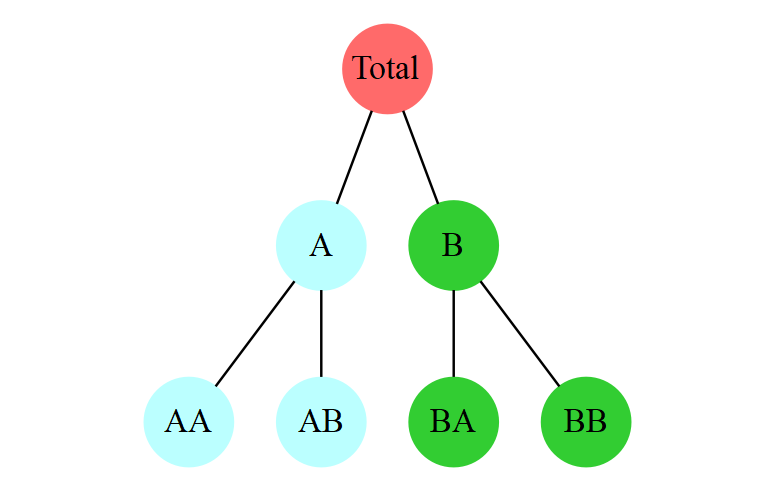
\includegraphics[width=3in]{Figures/treesimple}
	\caption{A 2 level hierarchical structure}
	\label{fig:treesimple}
\end{figure}

\newpara

Hierarchical relationship descripted in figure~\ref{fig:treesimple} can be presented with following equations:

\begin{equation}\label{equ:ts1}
\begin{aligned}
y_{total,t} = y_{A,t}+y_{B,t}
\end{aligned}
\end{equation}

\begin{equation}\label{equ:ts2}
\begin{aligned}
y_{A,t}=y_{AA,t}+y_{AB,t}\quad \quad y_{B,t}=y_{BA,t}+y_{BB,t}
\end{aligned}
\end{equation}

The relation can then be generalised into: , 

\begin{equation}\label{equ:Ts3}
\begin{aligned}
& y_{total,t} = \sum_{i=1}^{n_{i}} y_{i,t} \quad y_{i,t} = \sum_{j=1}^{n_{ij}} y_{ij,t} \quad... \\
\Rightarrow \quad & y_{parent,t} = \sum y_{children,t}
\end{aligned}
\end{equation}

Moreover, this can be thought of as aggregation constraints where observed values from bottom level hierarchies must sum to the observed value of the parent of these values. 


\newpara

Hierarchical time series can also be translated into a $n \times m$ matrix $S$, when $n$ equals to the number of observation of each time series, and when m equal to the total number of categories when considering categories from all levels \citep{Hydnman2016,wickramasuriya2019optimal}. For the hierarchical structure in Figure~\ref{fig:treesimple}, we can write with a matrix formula:
\begin{equation}\label{equ:Ts4}
\begin{aligned}
Y_t  \quad & \quad \quad \quad S \quad \quad \quad \quad b_t \\
\begin{bmatrix}
y_{Total,t} \\
y_{A,t}\\
y_{B,t} \\
y_{AA,t} \\
y_{AB,t}\\
y_{BA,t} \\
y_{BB,t}
\end{bmatrix}
= &
\begin{bmatrix}
1 & 1 & 1 & 1 \\
1 & 1 & 0 & 0 \\
0 & 0 & 1 & 1 \\
1  & 0  & 0  & 0  \\
0  & 1  & 0  & 0  \\
0  & 0  & 1  & 0  \\
0  & 0  & 0  & 1
\end{bmatrix}
\begin{bmatrix}
y_{AA,t} \\
y_{AB,t} \\
y_{BA,t} \\
y_{BB,t}
\end{bmatrix}\\
\end{aligned}
\end{equation}

\subsection{Forecasting approaches}

A classical method for hierarchical forecasting is the \textbf{bottom-up} approach. In this approach,  independent forecasts of each time-series series at the leaf(very bottom) level of the hierarchy are aggregate to workout the forecasts for the upper levels of the hierarchy until reaching the total. The main advantage of the approach is that no information is lost during the whole process; however, modelling and predictions of lower-level time-series often very challenging due to an abundant presence of noise \citep{hyndman2014optimally}. A level one level on top another level can be considered as the parent as it is where the lower level come from, vice versa a level one level below another level can be considered the children.  We can think of the hierarchical relationship, as shown in equation~\ref{equ:Ts5}, where the estimated values from the parent levels are the aggregations of estimates from children levels. 

\begin{equation}\label{equ:Ts5}
\begin{aligned}
\sum y_{children,t} \Rightarrow \quad & y_{parent,t} 
\end{aligned}
\end{equation}

\newpara

Another method for hierarchical forecasting is the \textbf{top-down} approach. In this approach, the forecast of each time-series series at the top level(total) is disaggregated down the hierarchy, with information of the hierarchical structure from historical data. This approach has reduced noise and is easier to model, but some information is lost during the process \citep{hyndman2014optimally}.  We can think of the relationship as shown in equation~\ref{equ:Ts6}, where the estimated values from the children level are comes from the dis-aggregations of estimates from the parent levels, given an estimation of a hierarchical structure $H$. 

\begin{equation}\label{equ:Ts6}
\begin{aligned}
\quad & y_{parent,t} | H \Rightarrow \sum y_{children,t} 
\end{aligned}
\end{equation}

\begin{figure}[!h]
	\centering
	\subfloat[Top down]{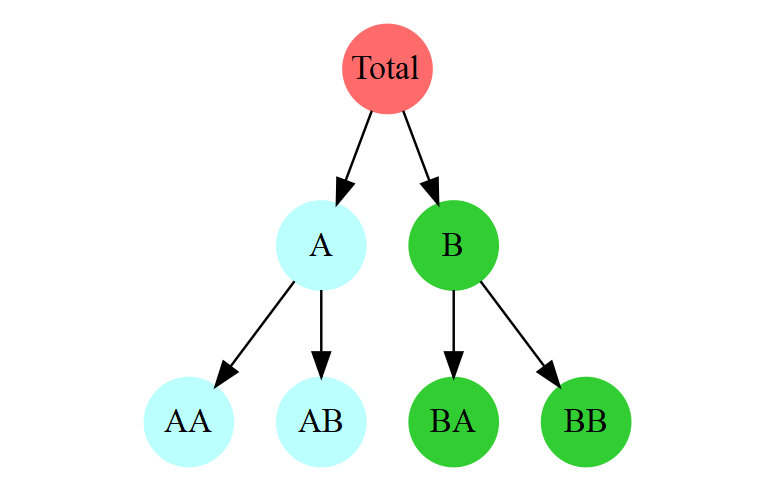
\includegraphics[width = 2in]{Figures/topdown}} 
	\subfloat[Bottom up]{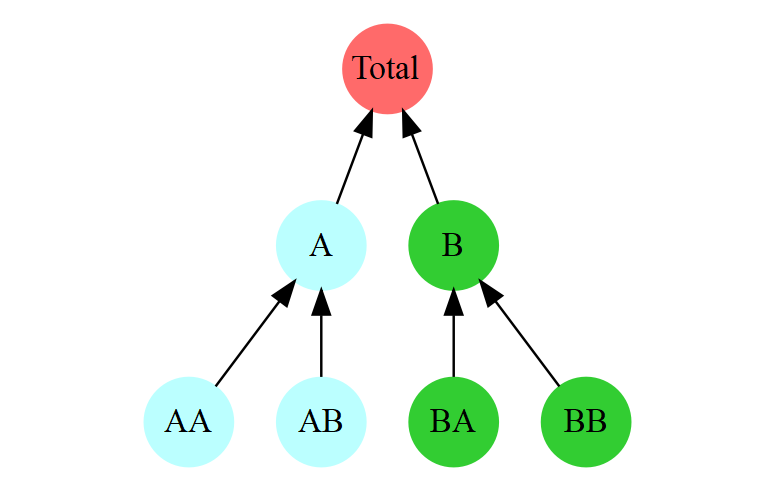
\includegraphics[width = 2in]{Figures/bottomup}}
	\subfloat[Optimum reconciliation]{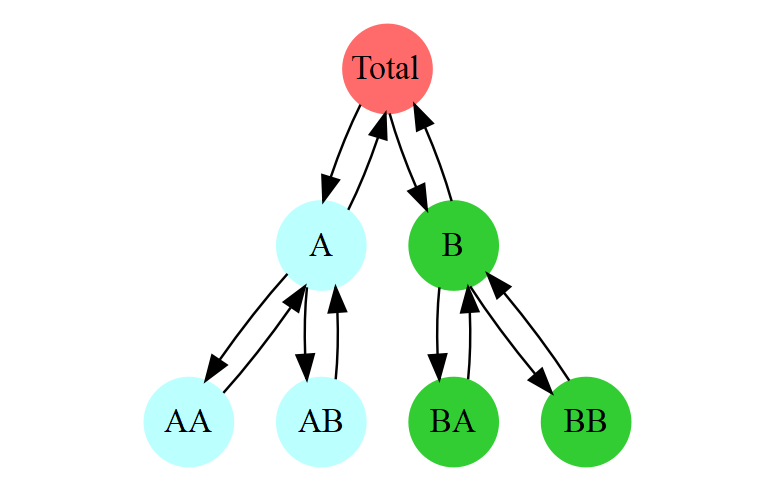
\includegraphics[width = 2in]{Figures/optim}}\\
	\caption{Top-down, Bottom up and Optimum reconciliation approach}
	\label{fig:approaches}
\end{figure}

\newpara 

\cite{hyndman2011optimal} recommend a new method of \textbf{optimal reconciliation} for the forecast of hierarchical time series data for its feature and performance. The optimal reconciliation works by independently forecasting each time-series at all levels of the hierarchy, and then reconcile each forecast with regression models by minimising the forecasting error (Figure~\ref{fig:approaches}). The most significant advantage the optimal reconciliation approach is that all of the information available within each level of the hierarchical structure are in consideration during the forecasting process. The idea is that important information may lye within any particular level within the whole hierarchical structure, and can be hard to detect from other levels if we only consider one level at the time \citep{hyndman2018forecasting}. A weakness of the optimal reconciliation is that even if the observations considered are natural numbers; it could still produce negative predictions that are the optimum solution to the prediction but does not make sense in real-life. In many instances, time-series predictions need a set of non-negative reconciled forecasts. If the demand for a particular commodity for the time-period $t = 2020$ is $-5$, it does not have any sense at all. 

\newpara

Time-series forecast with all approached mentioned above can be made by using the \texttt{forecast()} function with an \texttt{hts} object (created using \texttt{ts} and \texttt{hts} function)in under the \texttt{hts} package \citep {hts} in the R environment. Optimal non-negative reconciled forecasts are currently not available for the \texttt{hts} package within the R environment, but a little bird told me \texttt{hts} package with non-negative reconciled forecasts will be updated at the end of July 2019. For another note, optimum reconciliation forecasts used for the next session does have negative values, but the values are mostly extremely small so they are treated as 0 values. 



%------------------------------------------------------------------------------------------
\newpage
\section{Outline of Thesis}

The organisation of the thesis is described in the follows: 

\newpara

\ding{169} \textbf{\Cref{chap:Background}} starts with the introduction of examples of where these issues in hierarchical structure arise; these include background and concepts of the topics, including emergency department congestion and anomaly detection. Technical background about statistical methods and techniques necessary for our methods, these include topics of and within Bayesian inference and hierarchical time-series predictions. Lastly, we included outlines for the thesis and notations and conventions for this thesis. 

\newpara

\ding{169} \textbf{\Cref{chap:Simulations}} presents methods, results and discussion of our simulation studies of anomaly detection in several settings. The first simulation looks on how different priors would affect the goodness of fit and posterior results of Independent Bayesian Models(IBM). The second simulation compares scenarios with different increments of anomalies added. The third simulation compares scenarios with different different branching at Category A, with addition of a constant anomaly.

\newpara

\ding{169} \textbf{\Cref{chap:MIMIC}} presents methods, results and discussion of our studies of anomaly detection with MIMIC-III, a publicly-available database with health-related data. More specifically, for four scenarios which include original observations and observations with anomalies added on categories of common, rare and extremely rare disease diagnoses. 

\newpara

\ding{169} \textbf{\Cref{chap:Conclusion1}} provides a final conclusion and overview of studies presented in this thesis.

\newpara

\begin{itemize}
	\item  \textbf{The Appendix} includes:
	\begin{itemize}
		\item  Descriptions of custom R function created, and R code used to implement different prior models, Independent Bayesian Model and Hierarchical Bayesian Model, used in \Cref{chap:Simulations} and \Cref{chap:MIMIC}.
	\end{itemize}
\end{itemize}

%------------------------------------------------------------------------------------------
\newpage
\section{Notations and conventions}

The following notation and conventions are used throughout this thesis to aid\\ readability:

\newpara

\begin{tabular}{rl}
	\textbf{Software} & Software is denoted by mono-space font with boldface.\\
	& For example: This plot is created using \texttt{\textbf{R}} codes. \\
	
	&\\ 
	
	\textbf{R packages} & Package names are given in mono-space font .\\
	& For example: This function is from the \texttt{GOpro} package. \\
	
	&\\ 
	
	\textbf{R functions} & Functions are denoted with mono-space font with two trailing \\
	& parentheses. Arguments are similarly displayed in monospace \\
	& with format "value" or "argument = value".\\
	& For example: This plot is created using \texttt{ggplot()} function.\\
	& For example: We used \texttt{dnorm(1, sd = 0.1) as our hyper-prior} \\
	
	&\\ 
	
	\textbf{Quotes} & Direct quotes should be denoted using Italic font\\
	& For example: "\textit{Shall I compare thee to a summer’s day}" \\
	
	&\\
	
	\textbf{Textbooks} & Text book and journal titles should be denoted using Italic font\\
	& For example: "\textit{High Performance Computing for Disease Surveillance}" \\
	
	&\\
	
	\textbf{Key words} & Some key words are denoted in bold font\\
	& For example: We have \textbf{significant} results.  \\
	
\end{tabular}
	\chapter{Simulations}\label{chap:Simulations}

\section{Introduction}

In this chapter, we carried-out simulations with synthetic patient arrival datasets and compares the posterior distribution results and prediction rate between Independent Bayes Model (IBM) and Hierarchical Bayes Model (HBM) in scenarios of with different anomalies and different hierarchy structures. Sections 2.1 details functions used to synthesis simulation datasets. Sections 2.2 evaluate the use of different priors for Bayesian Models to used during the simulations. Section 2.3 explores the impact of the size of the anomaly on anomaly detection at different levels of hierarchy. Lastly, section 2.4 considers how the complexity of the hierarchical structure affects anomaly detection at different levels of hierarchy. 
%add \ref{} to sections

\section{Simulation Methods}

All datasets used for the simulation studies are synthetically generated. Synthetic datasets refer to data information artificially manufactured rather than generated from real-world events. Synthetic data takes preference over the alternative option, perturbed data, a dataset generated by adding alteration and noise to real-world data \citep{drechsler2008comparing, drechsler2011synthetic}. Advantages of synthetic data include (1) Disclosure protection, making sure no sensitive information about individuals from the public can not be leaked or extracted. (2) Reduce the effects of possible background noises presented in real-world data. (3) Allows control over the hierarchical structure of datasets, note that real-world hierarchical data are often extremely complex and can have lots of levels, and complexity that comes with it, increasing the difficulty to control our simulations, and making interpretations difficult.  


\newpara

Several custom R-functions has been created to synthesis datasets used in our studies,  Appendix~\ref{Rfun} provides descriptions of the custom functions. There are several reasons for creating custom simulation synthesis functions. Firstly, a large number of simulated datasets with variable settings were expected to be required to perform our analyses; this required a large number of custom function arguments that existing packages may not contain. Secondly, synthetic datasets were simulated to mimic a health dataset in a purely theoretical setting. Thirdly, an emphasis was placed on the hierarchical nature of particular variable of the dataset (for example, ICD codes and geographic location), custom structure hierarchical structures can be used to generate branching, and nodes during the simulation process. Lastly, for exploration research, it was unclear what functionalities were needed, existing statistical data simulation packages may become insufficient at a later stage.

\begin{figure}[!t]
	\centering
	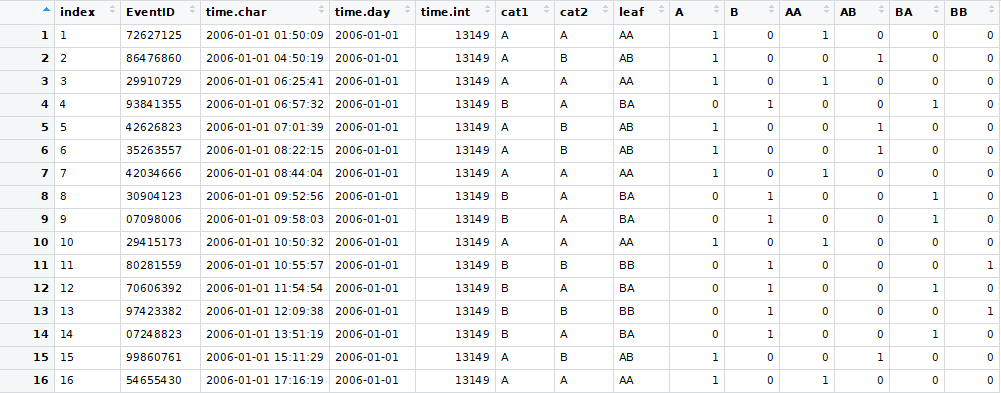
\includegraphics[width=1.0\linewidth]{Figures/rawdata}
	\caption{Entries of the raw dataset}
	\label{fig:rawdata}
\end{figure}

\newpara

\texttt{simdata} and \texttt{adddaily.anomaly} are the two major function used during the data synthesis process. \texttt{simdata} function were used to synthesise a raw dataset (figure~\ref{fig:rawdata}) that simulate a hospital record that you would typically found in hospital digital archives, where each row corresponds to a single entry of hospital event with a unique hospital event identifier. The function automatically generates Time, dates and various information about the hierarchical structure. The default number of simulation is 1,000,000, and default period is a 12 year-long period between 1 January 2006 and 31 December 2018, and a matrix that contains information of the hierarchical structure are manipulated and used to produce a hierarchical structure with different characteristics.

\newpara

The matrix used in the argument of \texttt{simdata} function contains the theoretical value of each leaf of a two-level hierarchical structure in a proportion out of 1000. This matrix is used to specify the hierarchical structure for each of our simulated data. As shown with the simplified example in  figure~\ref{fig:flow}, for example, if the theoretical value at of the leaves (refers to categories at the very bottom level hierarchy) are 8, 8, 5, and 3, the function will convert and  represent this information with a matrix with standard numbers 333,333,209 and 125. Each column corresponds to a single group; therefore, column sums of the matrix correspond to the count of a level 1 categories, and the sum of all numbers in the matrix equal to the total count. The parent levels are simply the sum of children levels, and the complete hierarchical structure can be generated automatically just from numerical information of leaves. Note that the number of column of the matrix corresponds to the maximum number of leaves within a level 1 category, for level 1 categories with less than maximum amount of leaves, 0 is used to represent no leaf. The default value of the matrix is 250, 250, 250 and 250, which represent a two-level hierarchical of equal proportions, with 2 level-1 categories, each with 2 level-1 categories of equal proportions.Note the function can be used to generate all possibilities of 2-level hierarchical model, not just the 4 leaf example that is shown here, the use of out of 1000 (instead of being four non-negative real numbers which add to 1, which makes better sense) is a personal choice because it makes coding easier. This way of storing hierarchical information is simple and efficient but is not suitable for hierarchical models that contain 3 or more levels, and maybe a little confusing for other people at first, future improvements of the function could be allowing usage of a user-generated hierarchical time series (\texttt{hts}) object from the \texttt{hts} package instead of the matrix, to allow generations of  hierarchical dataset with  3 or more levels. 

\newpara 

\begin{figure}[!t]
	\begin{equation*}
	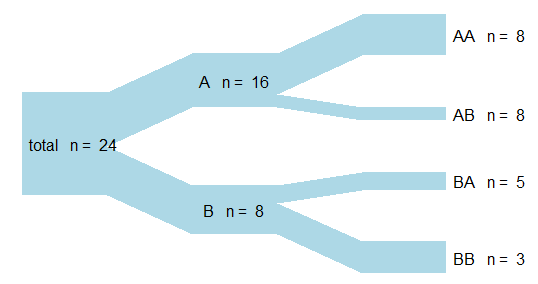
\includegraphics[width=0.7\linewidth]{Figures/flow1} 
	\Rightarrow
	\begin{bmatrix}
	8 & 5 \\
	8 & 3 \\
	\end{bmatrix}
	\Rightarrow
	\begin{bmatrix}
	333 & 208 \\
	333 & 125 \\
	\end{bmatrix}
	\end{equation*}
	\caption{Conversion of a simple hierarchical structure to a matrix}
	\label{fig:flow}
\end{figure}

\begin{figure}[!h]
	\centering
	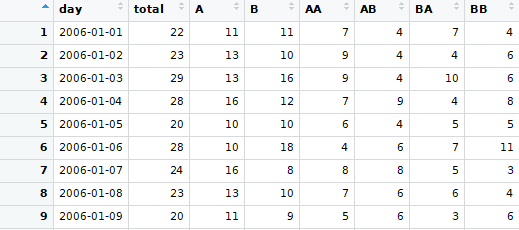
\includegraphics[width=0.7\linewidth]{Figures/dailydata}
	\caption{Entries of the daily count dataset}
	\label{fig:dailydata}
\end{figure}


\texttt{adddaily.anomaly} were used to \texttt{addanomaly} function to add anomaly to daily count data(number of hospital arrivals), a hierarchical time-series dataset generated by tabulating the raw synthesised dataset (with each entry representing a hospital arrival event)using \texttt{tabulatedata} function. The default setting for anomaly is a point anomaly of 1 day, on 2015-11-15. The amount of anomaly added are in terms of the proportion of the total count (For example, a 25\% anomaly here meant an addition of 25\% of the count of category total, on top of the hierarchy,in mathematical terms $1.25y_{total,t}$, in other words, if we expect 100 hospital arrival events, an arrival rate of 125 meant a 25\% anomaly has occurred), and amount of anomaly assigned to each leaf (subcategories, in this thesis, different ICD codes) can be varied. This controls the size of overall anomaly and allows for customisation of hierarchical structure at lower levels, the plan is to give the freedom to explore how different hierarchical structure would affect the results of our hierarchical and independent models. 


\newpara

For point anomalies the amount of anomaly assigned to each leaf is transcribed with binding of 3 vector: (1) a vector of amount of anomaly to be added to total,  (2) a vector of amount of anomaly to be added to level 1 categories and (3) a vector of amount of anomaly to be added to level 2 categories, all in values of proportions. In mathematical thinking, we could think of binding as additions of $n*m$ matrices, where information only exist on certain row or columns, and addition of the column or rows condense all the information together.  For example, for a hierarchical time series with the same hierarchical structure as the example given in figure \ref{fig:flow}, if we want to add all of our anomalies to AA, the proportion vector of anomaly for total is $\{1\}$ and this will be the case for any hierarchical structure because the proportion of all categories will sum to 1. The proportion vector of anomaly for level 1 categories is $\{1,0\}$ and the percentage vector for level 2 categories is $\{1,0,0,0\}$, so the proportion vector that is required for our function to indicate our setup, is $\{1,1,0,1,0,0,0\}$. 

\begin{figure}[!h]
	\begin{equation*}
	\begin{aligned}
	P_{total} \quad 
	P_{lv1} \quad \quad \quad \quad  
	P_{lv2} \quad \quad \quad & 
	\quad \quad \quad  \quad \quad  P \\
	\begin{bmatrix}
	1 \\
	\end{bmatrix}
	+
	\begin{bmatrix}
	1 & 0\\
	\end{bmatrix}
	+
	\begin{bmatrix}
	1 & 0 & 0 & 0\\
	\end{bmatrix}
	\Rightarrow &
	\begin{bmatrix}
	1 & 1 & 0 & 1 & 0 & 0 & 0\\
	\end{bmatrix}
	\end{aligned}
	\end{equation*}
	\caption{Construction of the proportion vector}
	\label{fig:vec}
\end{figure}

In summaries, \texttt{simdata} and several supporting functions were used to generate simulated data, and then we manually added different anomalies with \texttt{adddaily.anomaly} function. The whole process resulted in 60 various simulated datasets with same default setting (refer to details on \texttt{simdata}), different hierarchical structure and different added anomalies that are used for this section. 

\newpara

Details about setups used for the data synthesis process can be found in the start of each section of our simulation tests, and the R codes used can be found in \texttt{91-createdata-test.R}, \texttt{92-createdata-anoamly.R}, \texttt{93-createdata-proportion.R} and \texttt{94-createdata-count.R} found in GitHub Repository: \href{https://github.com/jungxue/research-masters-Jung}{https://github.com/jungxue/ research-masters-Jung}. 

%------------------------------------------------------------------------------------------        
\newpage

\section{Simulation 1: Prior}

\subsection{Priors}

For Bayesian inference to make sense, a prior is essential and often required. However, there are different ways in which prior can be generated. For simulations, no external information is available; therefore, the informative prior approach is out of the question. However, it is possible for us to assign relatively simple weak-informative and non-informative priors by generating probability distributions with vaguely defined parameters. Hence, we proposed six different priors that express different hypothesised information about the prior and test how they affect our posterior distribution calculations. 
\newpara

A simple Poisson process can be used to model for a random, and mutually independent arrivals rate, with the likelihood model:

\begin{equation*} \label{Poisson}
\begin{aligned}
y_{,t} & \sim Poisson(\mu_{i,t}) \\  
log(\mu_{i,t}) & = log(\rho_{i,t}) \\
\end{aligned}
\end{equation*}

For the Poisson process, observations $y_{i,t}$ ($y$ of $i$th category given time $t$) is hypothesised to follow the distribution of the Poisson process, with parameter $\mu_{i,t}$ stand for the expected number of arrivals per time-interval(In this study we are actually only looking at one particular day/time interval, so t actually does not vary, but the notation is still included to make general sense) And $\rho_{i,t}$ as the log equivalent. For our simulations, this time interval is set up to be a 12 year-long period between 1 January 2006 and 31 December 2018.The sum of simulated arrival entries sum to 1,000,000. Distributions of priors can then assigned to $\mu_{i,t}$, this provides essential information to the parameter and will have a significant impact in our calculations. Samples of the JAG codes used to build our models is presented in appendix~\ref{models}, and complete JAGS codes and R codes used to obtain our graphical results are available on GitHub repository:
\href{https://github.com/jungxue/research-masters-Jung}{https://github.com/jungxue/research-masters-Jung}. 

\subsubsection{Model 1 Non-informative Prior}

Model 1 is an Independent Bayesian Model with no priors that models each categories independently on all hierarchical levels. This model provides no information for the estimation of distribution parameter $\mu_{i,t}$, and therefore the prior can be defined as a non-informative prior (although this term often refers to flat prior), here in this thesis we call it the null prior. The likelihood model for Poisson model with null prior is:

\begin{equation*} \label{Poissonm1}
\begin{aligned}
y_{i,t} & \sim Poisson(\mu_{i,t}) \\  
log(\mu_{i,t}) & = log(\rho_{i,t}) \\
\end{aligned}
\end{equation*}

\subsubsection{Model 2 Normal($\mu$=1,$\sigma^-2$=0.3) Prior}

Model 2 is an Independent Bayesian Model with $\rho \sim Normal(1, 0.3)$ prior that models each categories independently on all hierarchical levels. This model does contain information for the estimation of distribution parameter $\mu_{i,t}$, and therefore the prior can be defined as a weak-informative prior. $I_{[\lambda>0]}$ indicates truncation of distribution at 0; in other words, the prior does not contain$\lambda_{i,t}$ with values less than 0 and should not contain any negative values. The likelihood model for a Poisson process with a $Normal(1, 0.3)$ prior is:

\begin{equation*} \label{Poissonm2a}
\begin{aligned}
y_{i,t} & \sim Poisson(\mu_{i,t}) \\  
log(\mu_{i,t}) & = log(\rho_{i,t}\lambda_{i,t}) \\
\end{aligned}
\end{equation*}

Priors for model parameters:

\begin{equation*} \label{Poissonm2b}
\begin{aligned}
\lambda_{i,t} & \sim Normal(\mu_{i,t},\sigma_{i,t}) I_{[\lambda>0]}\\
\end{aligned}
\end{equation*}

Hyper-priors for model parameters:

\begin{equation*} \label{Poissonm2c}
\begin{aligned}
\mu_{i,t} & \sim Normal(1,0.1)\\
\sigma^2_{i,t} &\sim Normal(0.3,0.1)\\
\end{aligned}
\end{equation*}

\subsubsection{Model 3 Normal($\mu$=1,$\sigma^-2$=0.1) Prior}

Model 3 is an Independent Bayesian Model with $\rho \sim Normal(1, 0.1)$ priors that models each categories independently on all hierarchical levels. This model does contain information for the estimation of distribution parameter $\mu_{i,t}$, and therefore the prior can be defined as a weak-informative prior. $I_{[\lambda>0]}$ indicates truncation of distribution at 0; in other words, the prior does not contain$\lambda_{i,t}$ with values less than 0 and should not contain any negative values. The likelihood for a Poisson process with a $Normal(1, 0.1)$ prior model is:

\begin{equation*} \label{Poissonm3a}
\begin{aligned}
y_{i,t} & \sim Poisson(\mu_{i,t}) \\  
log(\mu_{i,t}) & = log(\rho_{i,t}\lambda_{i,t}) \\
\end{aligned}
\end{equation*}

Priors for model parameters:

\begin{equation*} \label{Poissonm3b}
\begin{aligned}
\lambda_{i,t} & \sim Normal(\mu_{i,t},\sigma_{i,t}) I_{[\lambda>0]}\\
\end{aligned}
\end{equation*}

Hyper-priors for model parameters:

\begin{equation*} \label{Poissonm3c}
\begin{aligned}
\mu_{i,t} & \sim Normal(1,0.1)\\
\sigma^2_{i,t} &\sim Normal(0.1,0.1)\\
\end{aligned}
\end{equation*}

\subsubsection{Model 4 Gamma($alpha$=4,$beta$=3) Prior}

Model 4 is an Independent Bayesian Model with $\rho \sim Gamma(4, 3)$ priors that models each categories independently on all hierarchical levels. This model does contain information for the estimation of distribution parameter $\mu_{i,t}$, and therefore the prior can be defined as a weak-informative prior. $I_{[\lambda>0]}$ indicates truncation of distribution at 0; in other words, the prior does not contain$\lambda_{i,t}$ with values less than 0 and should not contain any negative values. The likelihood model for Poisson process with  $Gamma(4, 3)$ prior is:

\begin{equation*} \label{Poissonm4a}
\begin{aligned}
y_{i,t} & \sim Poisson(\mu_{i,t}) \\  
log(\mu_{i,t}) & = log(\rho_{i,t}\lambda_{i,t}) \\
\end{aligned}
\end{equation*}

Priors for model parameters:

\begin{equation*} \label{Poissonm4b}
\begin{aligned}
\lambda_{i,t} & \sim Gamma(\alpha_{i,t},\beta_{i,t}) I_{[\lambda>0]}\\
\end{aligned}
\end{equation*}

Hyper-priors for model parameters:

\begin{equation*} \label{Poissonm4c}
\begin{aligned}
\alpha_{i,t} & \sim Normal(4,0.1)\\
\beta_{i,t} &\sim Normal(3,0.1)\\
\end{aligned}
\end{equation*}

\subsubsection{Model 5 Laplace($alpha$=1,$beta$=1) Prior}

Model 5 is an Independent Bayesian Model with $\rho \sim Laplace(1, 1)$ priors that models each categories independently on all hierarchical levels. This model does contain information for the estimation of distribution parameter $\mu_{i,t}$, and therefore the prior can be defined as a weak-informative prior. $I_{[\lambda>0]}$ indicates truncation of distribution at 0; in other words, the prior does not contain$\lambda_{i,t}$ with values less than 0 and should not contain any negative values. The likelihood model for Poisson process with $Laplace(1, 1)$ prior is:

\begin{equation*} \label{Poissonm5a}
\begin{aligned}
y_{i,t} & \sim Poisson(\mu_{i,t}) \\  
log(\mu_{i,t}) & = log(\rho_{i,t}\lambda_{i,t}) \\
\end{aligned}
\end{equation*}

Priors for model parameters:

\begin{equation*} \label{Poissonm5b}
\begin{aligned}
\lambda_{i,t} & \sim Laplace(\alpha_{i,t},\beta_{i,t}) T_{[\lambda>0]}\\
\end{aligned}
\end{equation*}

Hyper-priors for model parameters:

\begin{equation*} \label{Poissonm5c}
\begin{aligned}
\alpha_{i,t} & \sim Normal(4,0.1)\\
\beta_{i,t} &\sim Normal(3,0.1)\\
\end{aligned}
\end{equation*}

\subsubsection{Model 6 Mixture Prior}

Lastly, Model 6 is an Independent Bayesian Model with a mixture prior that models each category independently on all hierarchical levels. The prior is thought to be a mixture of no information and weak information, in other words, we are proposing that for most of the time there is no variation, and for some of the time, there is information. The idea comes from \citet{berry2004}, where they proposed a scenario where the majority of the difference between treatment and control is zero, and there are just some variations. However note that their prior is an one-sided distribution that centre at 0, and our prior is two-sided and centre at 1. This model does contain information for the estimation of distribution parameter $\mu_{i,t}$, and therefore, the prior can be defined as a weak-informative prior. $I_{[\lambda>0]}$ indicates truncation of distribution at 0; in other words, the prior does not contain$\lambda_{i,t}$ with values less than 0 and should not contain any negative values. The likelihood model for a Poisson model process with mixture prior is:

\begin{equation*} \label{Poissonm6a}
\begin{aligned}
y_{i,t} & \sim Poisson(\mu_{i,t}) \\  
log(\mu_{i,t}) & = log(\rho_{i,t}\lambda_{i,t}) \\
\end{aligned}
\end{equation*}

Priors for model parameters:

\begin{equation*} \label{Poissonm6b}
\begin{aligned}
\lambda_{i,t} & \sim Normal(spike_{i,t} + (1 - spike_{i,t})slab_{i,t}, 0.1) T_{[\lambda>0]} \\
\end{aligned}
\end{equation*}

Hyper-priors for model parameters:

\begin{equation*} \label{Poissonm6c}
\begin{aligned}
spike_{i,t} & \sim Binomial(0.9,1)\\
slab_{i,t} &\sim Normal(\mu_{i,t},\sigma_{i,t})\\
\end{aligned}
\end{equation*}

Hyper-hyper-priors for model parameters:

\begin{equation*} \label{Poissonm6d}
\begin{aligned}
\mu_{i,t} & \sim Normal(1,0.1)\\
\sigma^2_{i,t} &\sim Normal(0.1,0.1)\\
\end{aligned}
\end{equation*}

\newpage
\begin{figure}[!h]
	\centering
	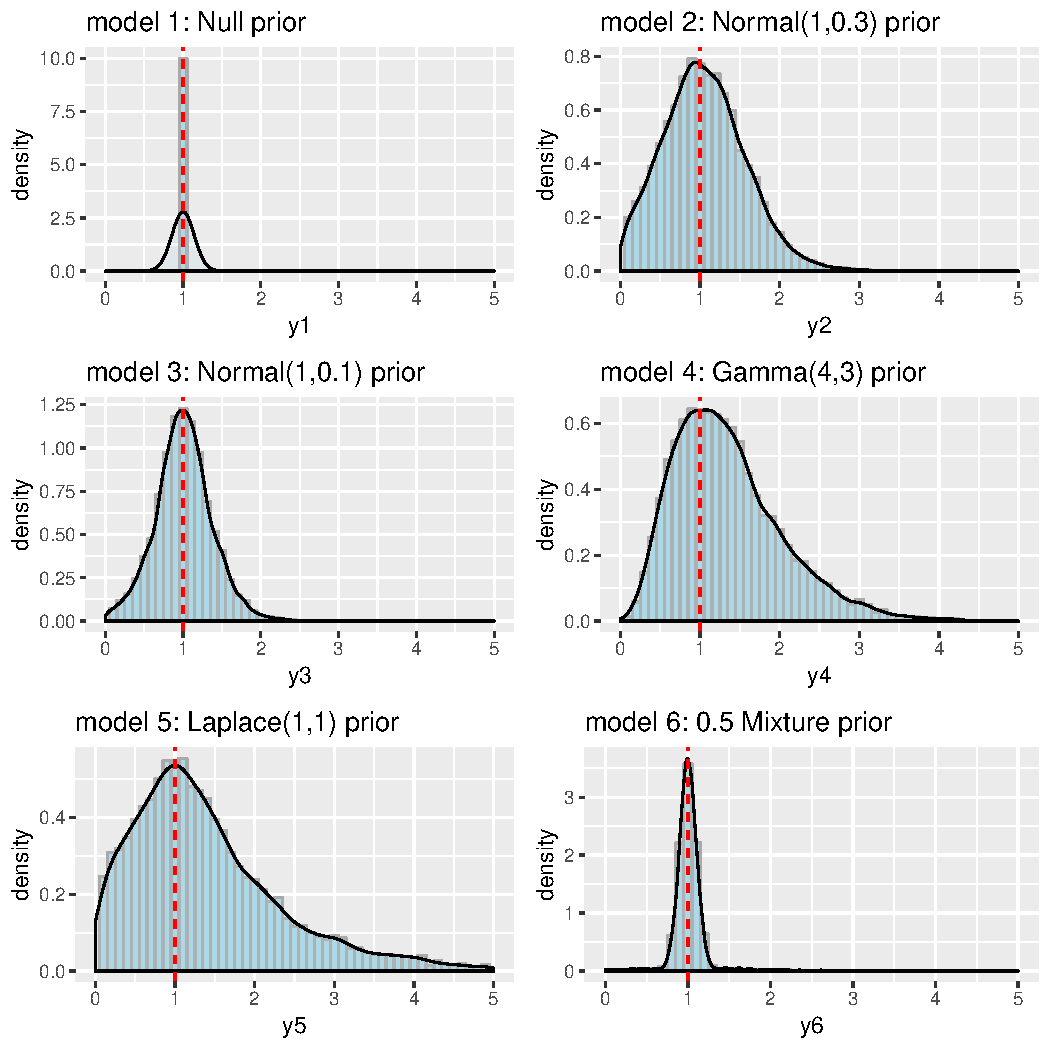
\includegraphics[width=1\linewidth]{../../R-codes/JAGS/plots/priordist}
	\caption{Histo-density plot of the prior probability distribution of proposed prior density models. The red dashed line indicates the center point of these distributions, which is 1.}
	\label{fig:priordist2}
\end{figure}

%---------------------------------------------------------------------------------------
Figure~\ref{fig:priordist2} show the distribution of $\lambda_{i,t}$ with hypothesised distributions just discussed, in histograms. Because we assign a prior distribution to our $\mu_{i,t}$ by directly multiplying by $\lambda_{i,t}$, the distribution of $\lambda_{i,t}$ is thought as the equivalent to the distribution of our prior. As presented in histograms, our priors have different distributions that suggest a different belief. Model 1 used a non-informative flat prior, that contains no information, and hence no distribution is observed, and only have 1 bar at 0. Model 2 used a $Normal(1, 0.3)$ prior that seems reasonable; however note that, because its left tail was truncated at 0, the distribution has lost its symmetrical property. Model 3 used a $Normal(1, 0.1)$ that has a smaller variance, hence the distribution is a little bit taller, indicating more observation tend to be close to the mean. Model 4 used a $Gamma(4, 3)$ prior; it skews towards the right-hand side. The distribution translates into that we are observing more positive anomalies compare to negative anomalies. Model 5 used a $Laplace(4, 3)$ prior, it also skews to the right, but with a heavier tail and a much higher distribution at extreme positive values, this translates into information at we are consistently observing a large anomaly. Lastly, we have model 6 that used a mixture prior; there is a very strong spike at 1 and some variation around it.

\subsection{Simulation setups }

In section 2.3, we present the results of the posterior distribution calculations for the synthesised data, with anomalies added on category AA on level 2 (leaf) of the hierarchy. The default setting for the data synthesis process is applied, with the addition of 25\% anomaly. An important note, the 25\% anomaly here meant an addition of 25\% of the count of category total on top of the hierarchy, not addition of 25\% on category AA. In mathematical terms, a 25\% anomaly would be equivalent to $1.25 y_{total,t}$. 

\subsection{Results}

\begin{table}[ht]
	\centering
	\begin{tabular}{crrrrrr}
		\hline
		Comparisons & Min. & 1st Qu. & Median & Mean & 3rd Qu. & Max. \\ 
		\hline
		M1:M2 & -2.126 & -1.574 & -0.599 & -0.868 & -0.158 & 0.113 \\ 
		M1:M3 & -4.456 & -3.295 & -2.069 & -2.032 & -0.650 & 0.189 \\ 
		M1:M4 & -2.992 & -1.729 & -1.174 & -1.303 & -0.800 & 0.106 \\ 
		M1:M5 & -2.645 & -1.745 & -0.764 & -1.172 & -0.590 & -0.124 \\ 
		M1:M6 & -3.383 & -2.200 & -1.645 & -1.683 & -1.047 & -0.258 \\ 
		M2:M3 & -4.555 & -2.288 & -1.884 & -1.164 & 0.713 & 1.440 \\ 
		M2:M4 & -2.393 & -1.009 & -0.552 & -0.434 & -0.155 & 2.232 \\ 
		M2:M5 & -2.382 & -0.494 & -0.071 & -0.304 & 0.267 & 0.782 \\ 
		M2:M6 & -3.331 & -1.571 & -0.626 & -0.815 & -0.122 & 1.639 \\ 
		M3:M4 & -2.450 & -0.285 & 0.895 & 0.730 & 1.787 & 3.658 \\ 
		M3:M5 & -1.020 & -0.578 & -0.168 & 0.860 & 2.345 & 3.677 \\ 
		M3:M6 & -1.995 & -1.322 & -0.412 & 0.349 & 1.649 & 4.198 \\ 
		M4:M5 & -1.884 & -0.905 & 0.501 & 0.131 & 0.913 & 2.282 \\ 
		M4:M6 & -2.858 & -1.537 & -0.829 & -0.380 & 1.029 & 2.039 \\ 
		M5:M6 & -3.259 & -0.929 & -0.672 & -0.511 & 0.378 & 1.454 \\ 
		\hline
	\end{tabular}
	\caption{DIC (with 1,000,000 iteration) summary distribution cross comparisons for model 1 to model 6} 
	\label{tab:dic1}
\end{table}

\newpage

Table~\ref{tab:dic1} gives the comparison of of DIC distributions. A comparison of M1: M2 indicated comparisons between model 1 and model 2, with DIC distribution of model 2 taking away the DIC distribution of model 1. An important note to take before the interpretation of results in this table is the weak signals (a negative value signals a model is better than another) of the DIC estimations. The initial DIC results with 1000 iterations give weak signals, showing signs of slow convergence, this meant that the absoulute DIC values for each model differ by a large margin each time DIC ran for different jags model. Due to convergence and size of numbers it is difficult for human eye to read the difference between numbers. Using the difference of values between models instead of absolute values of each model, sometimes we get negative mean and median values, and sometimes we get positive mean and median values, a negative value indicate second model is better than first model, and size of number indicate the size of difference, making it easier to interpret. Weak signals are still present when the number of iteration increase to 1,000,000. With repeated trials, Model 2 to model 6 consistently gives a lower DIC value compares to model 1, showing strong signals at 3rd Quartile and Max value. The observation provides strong evidence that Model 1 with non-informative prior gives the highest and worse DIC estimations out of all models. The DIC comparisons for model 2 to model 6 have weak signals on mean and median values, even with high iterations, and it is almost impossible to tell the difference, this suggests that there is no or close to no difference between the DIC values for model 2 to model 6. 

%-------------------------- Posterior dist total------------------------------------------------
\newpage %

\begin{table}[!ht]
	\centering
	\begin{tabular}{rrrrrrrr}
		\hline
		& mean & sd & 2.5\% & 50\% & 97.5\% & Rhat & n.eff \\ 
		\hline
		model 1 & 21.0615 & 0.0000 & 21.0615 & 21.0615 & 21.0615 &  & 0 \\ 
		model 2 & 24.4976 & 4.7805 & 15.7987 & 24.2398 & 34.1927 & 1 & 3119 \\ 
		model 3 & 24.3373 & 4.9322 & 15.7804 & 23.9781 & 34.8648 & 1 & 3009\\ 
		model 4 & 24.1116 & 4.8248 & 15.5574 & 23.7915 & 34.4035 & 1 & 3587 \\ 
		model 5 & 24.4041 & 4.9549 & 15.9001 & 24.1139 & 34.7204 & 1 & 3152 \\ 
		model 6 & 24.8840 & 4.9712 & 16.4075 & 24.5082 & 35.4618 & 1& 2895 \\ 
		\hline
	\end{tabular}
	\caption{Posterior distributions of different models for Total, with added anomalies, and calculated with independent Bayes model} 
	\label{tab:modelpost1}
\end{table}

\begin{figure}[!h]
	\centering
	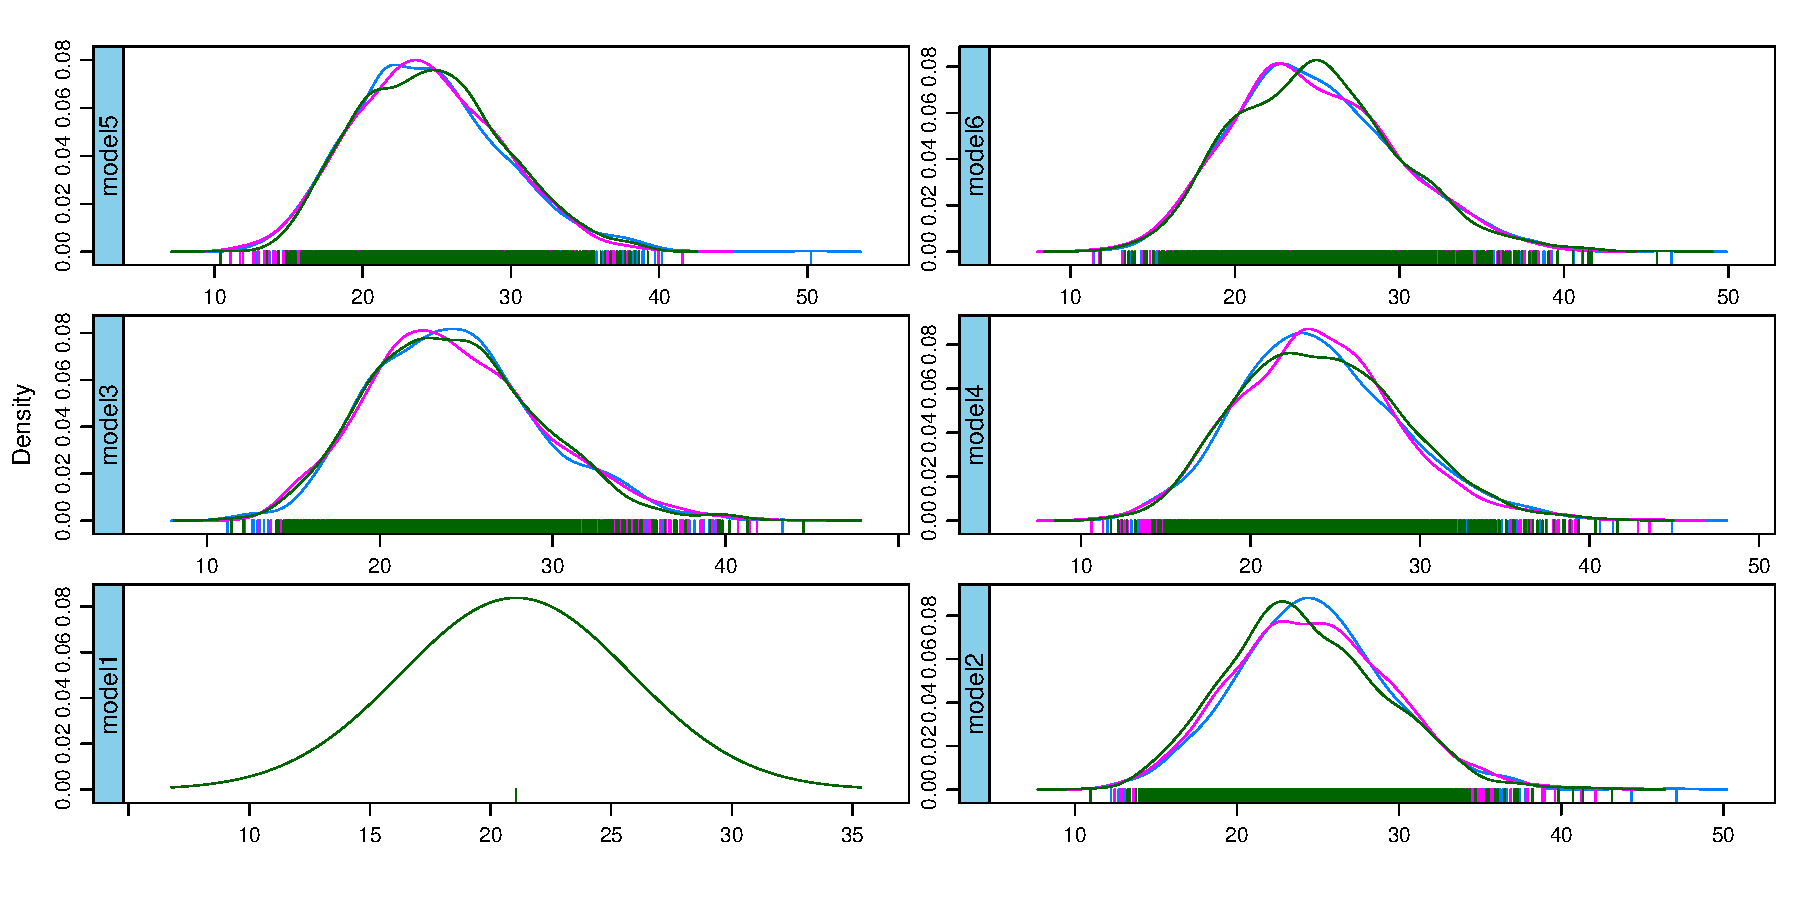
\includegraphics[width=1\linewidth]{../../R-codes/JAGS/plots/findmodel/Densitytotal3abn}
	\caption{Posterior distributions of different models for Total, with added anomalies, and calculated with independent Bayes model}
	\label{fig:densitytotal3abn}
\end{figure}

Table~\ref{tab:modelpost1} and figure~\ref{fig:densitytotal3abn} gives the posterior distribution of the category total, for each of the model. Model 1 uses non-informative prior, and it gives the most particular posterior out of all models at level 0 (total), the mean value of the posterior distribution is around 4.5 unit lower than other models, there is no standard deviation, and the number of effective samples is 0. Our observation suggests that non-informative priors produce a significantly different result compares to weakly informative priors. Posterior distributions for model 2 to model 6 are very similar and very hard to tell any significant difference, other than there seems to be a large difference between the number of effective sample size.

\newpage %----------------------------Posterior dist A ----------------------------------------------
\begin{table}[!ht]
	\centering
	\begin{tabular}{rrrrrrrr}
		\hline
		& mean & sd & 2.5\% & 50\% & 97.5\% & Rhat & n.eff \\ 
		\hline
		model 1 & 10.5463 & 0.0000 & 10.5463 & 10.5463 & 10.5463 &  & 0 \\ 
		model 2 & 12.3481 & 3.5241 & 6.4608 & 12.0826 & 19.7636 & 1 & 2833 \\ 
		model 3 & 12.2433 & 3.5058 & 6.3331 & 11.9460 & 20.1100 & 1 & 2955 \\ 
		model 4 & 12.0331 & 3.2668 & 6.4515 & 11.7501 & 19.1090 & 1 & 3322 \\ 
		model 5 & 12.3475 & 3.5362 & 6.4799 & 12.0049 & 19.9832 & 1 & 2503 \\ 
		model 6 & 12.9588 & 3.6536 & 6.8353 & 12.6056 & 21.2272 & 1 & 3000 \\ 
		\hline
	\end{tabular}
	\caption{Posterior distributions of different models for A , with added anomalies, and calculated with independent Bayes model} 
	\label{tab:modelpost2}
\end{table}

\begin{figure}[!h]
	\centering
	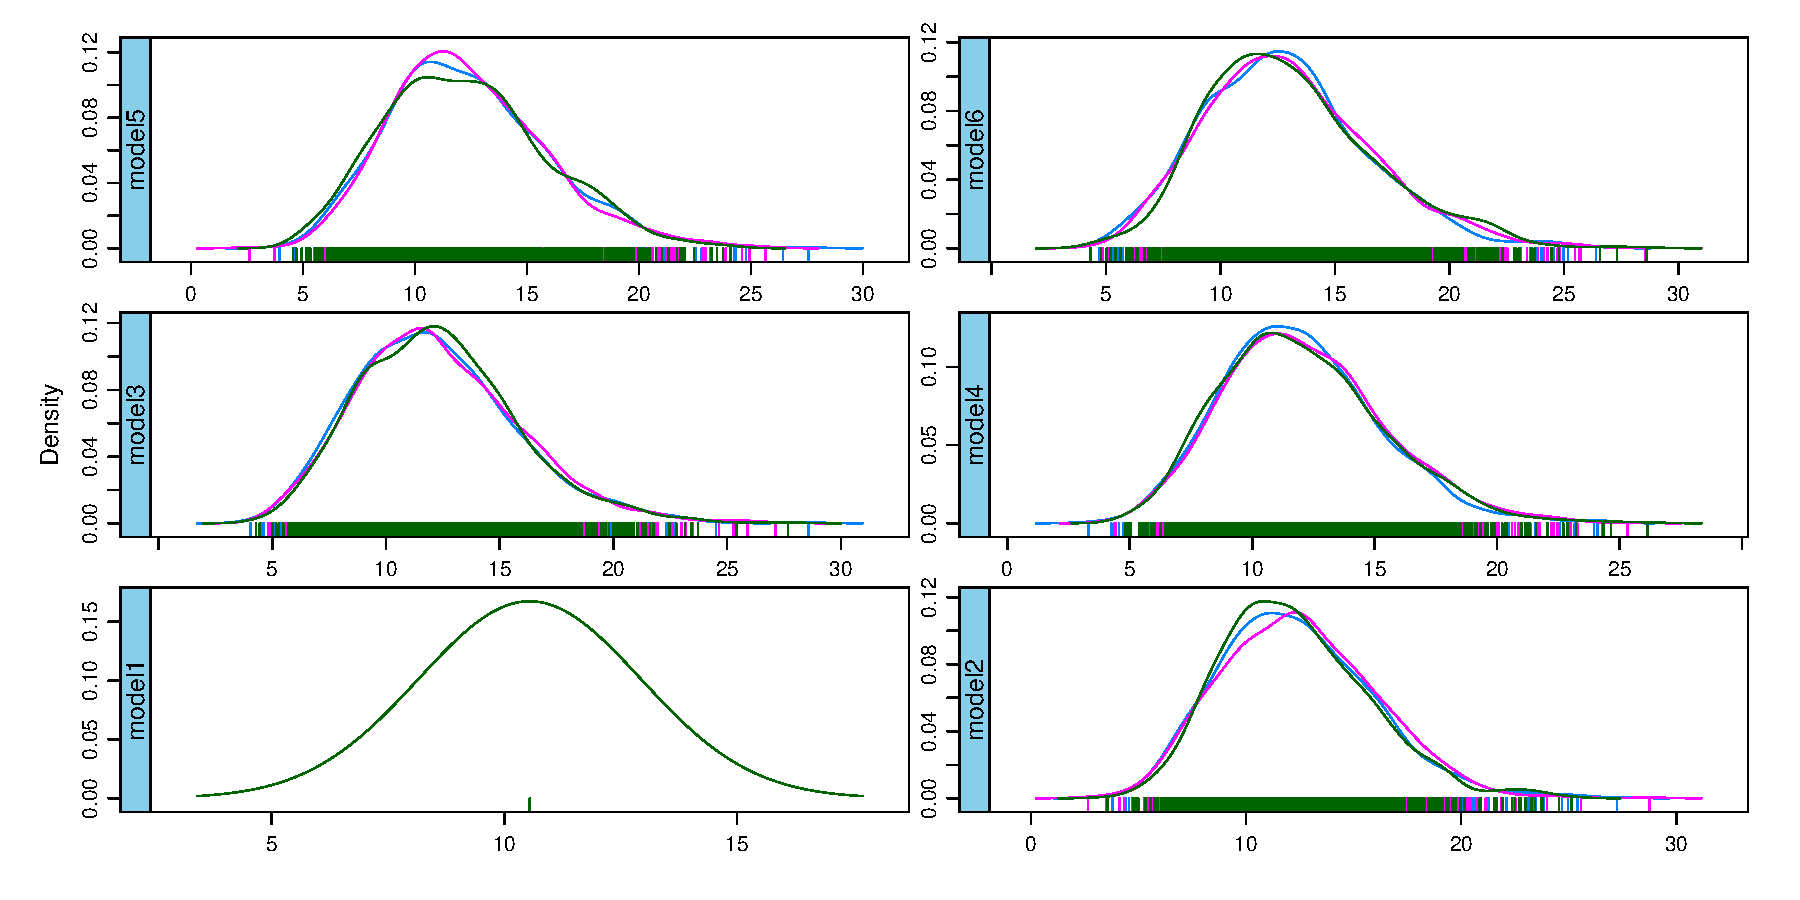
\includegraphics[width=1\linewidth]{../../R-codes/JAGS/plots/findmodel/DensityA3abn}
	\caption{Posterior distributions of different models for A , with added anomalies, and calculated with independent Bayes model}
	\label{fig:densityA3abn}
\end{figure}

Table~\ref{tab:modelpost2} and figure~\ref{fig:densityA3abn} gives the posterior distribution of the category A, for each of the model. Model 1 uses non-informative prior, and it gives the most particular posterior out of all models at level 1 (A), the mean value of the posterior distribution is around 2 unit lower than other models, there is no standard deviation, and the number of effective samples is 0. Our observation suggests that non-informative priors produce a significantly different result compares to weakly informative priors. Posterior distributions for model 2 to model 6 are very similar and very hard to tell any significant difference, other than there seems to be a large difference between the number of effective sample size.

\newpage %--------------------------- Posterior dist AA -----------------------------------------------
\begin{table}[!ht]
	\centering
	\begin{tabular}{rrrrrrrr}
		\hline
		& mean & sd & 2.5\% & 50\% & 97.5\% & Rhat & n.eff \\ 
		\hline
		model 1 & 5.2477 & 0.0000 & 5.2477 & 5.2477 & 5.2477 &  & 0 \\ 
		model 2 & 7.4081 & 2.7444 & 2.8634 & 7.1136 & 13.3165 & 1 & 2273 \\ 
		model 3 & 7.3234 & 2.7423 & 2.8910 & 7.0234 & 13.3408 & 1 & 2372 \\ 
		model 4 & 6.9192 & 2.4111 & 3.0404 & 6.6744 & 12.3585 & 1 & 3000 \\ 
		model 5 & 7.6640 & 2.8689 & 3.0550 & 7.2466 & 14.0954 & 1 & 1886 \\ 
		model 6 & 7.8524 & 2.7397 & 3.4434 & 7.5279 & 14.0425 & 1 & 2856 \\ 
		\hline
	\end{tabular}
	\caption{Posterior distributions of different models for AA, with added anomalies, and calculated with independent Bayes model} 
	\label{tab:modelpost3}
\end{table}

\begin{figure}[!h]
	\centering
	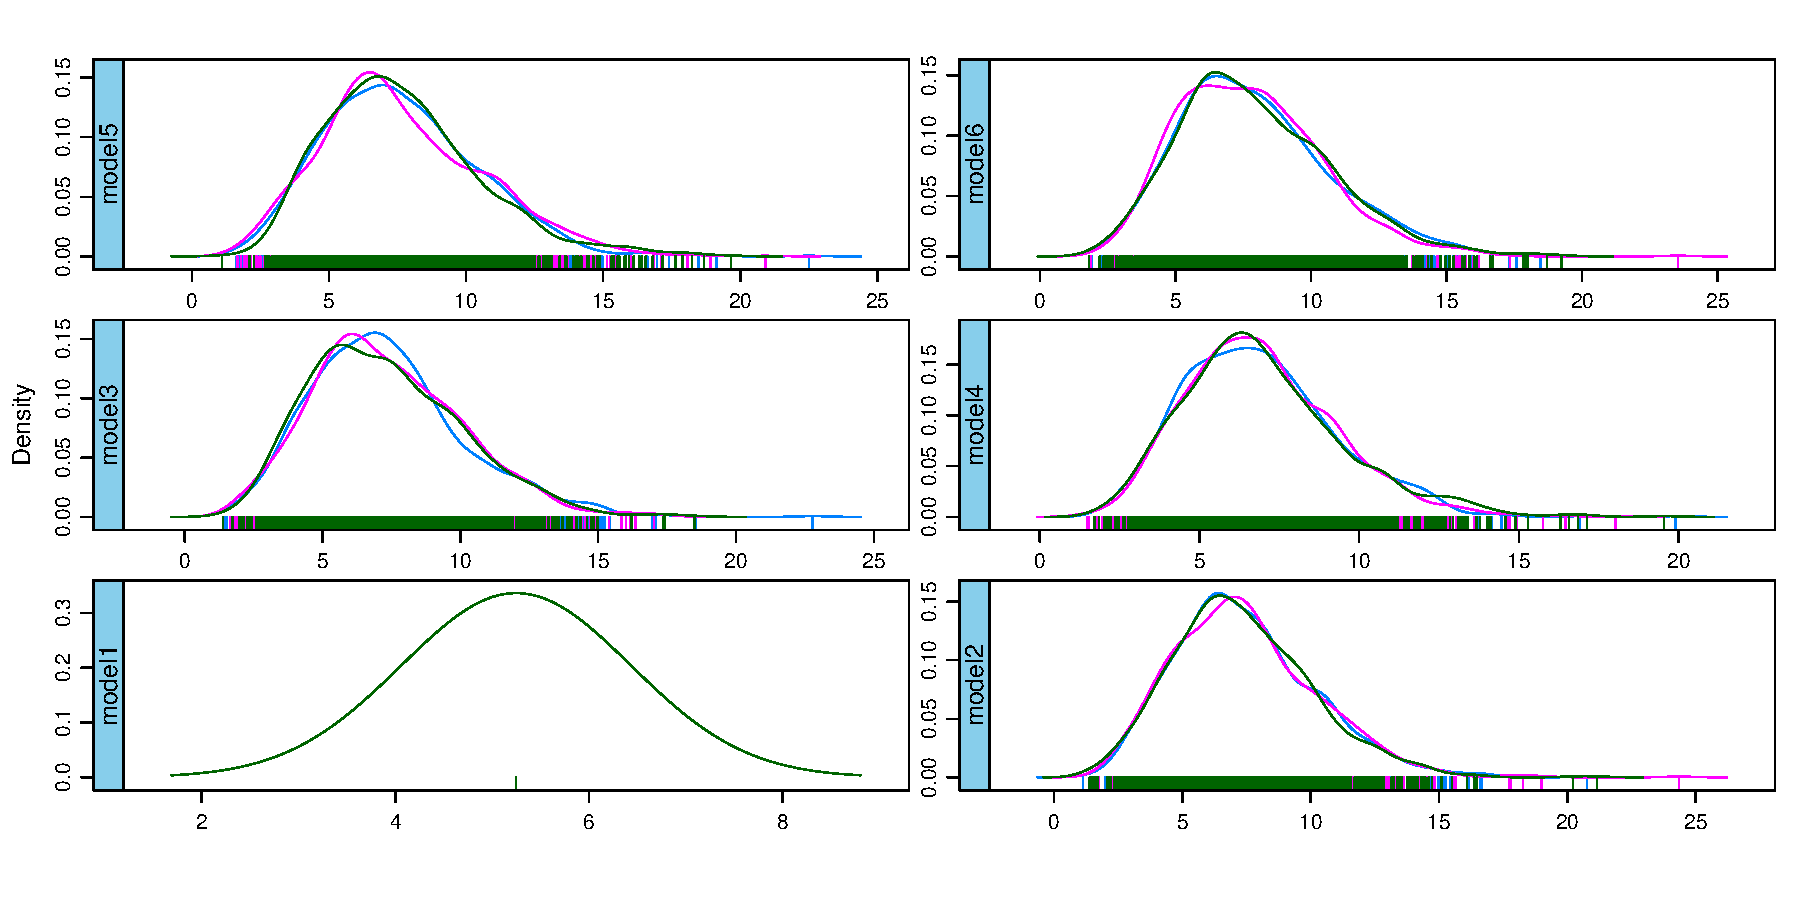
\includegraphics[width=1\linewidth]{../../R-codes/JAGS/plots/findmodel/DensityAA3abn}
	\caption{Posterior distributions of different models for AA, with added anomalies, and calculated with independent Bayes model}
	\label{fig:densityAA3abn}
\end{figure}

Table~\ref{tab:modelpost3} and figure~\ref{fig:densityAA3abn} gives the posterior distribution of the category AA, for each of the model. Model 1 uses non-informative prior, and it gives the most particular posterior out of all models at level 2 (AA), the mean value of the posterior distribution is around 2 unit lower than other models, there is no standard deviation, and the number of effective samples is 0. Our observation suggests that non-informative priors produce a significantly different result compares to weakly informative priors. Posterior distributions for model 2 to model 6 are very similar and very hard to tell any significant difference, other than there seems to be a large difference between the number of effective sample size.

\newpage

Considering posterior distribution results of all three hierarchical levels, it is apparent that Model 1 gives a significantly different posterior compares to all other models, suggesting that the usage of non-informative prior will generate significantly different results compares to weakly informative priors at all levels of Hierarchy. Model 2 to model 6 gives similar posterior distribution, with similar numeric values in tables and similar shapes in density plots in all levels, this suggests that there no or close to no differences between the posterior distributions of Model 2 to model 6 and using slightly different weakly informative prior does not make a significant impact on our posterior distribution results in all levels of hierarchy. The mean and standard deviation of posteriors for model 2 to model 6 decreases as the level of hierarchy increase (going down the hierarchy), with category total having the largest mean and standard deviation, category A having smaller mean and standard deviation, and category AA having the smallest mean and deviation. Our observation makes sense as the aggregation constraints of hierarchical datasets dictates that the mean and sample size of categories at higher hierarchy will always be greater than mean and sample size of categories at the lower hierarchy. The number of effective size for model 2 to 6 seem to decrease as the level of hierarchy increase, which made sense because due to aggregation constraints, observed values at a lower hierarchy tend to be smaller and less variable, and this will produce a stronger autocorrelation during the MCMC process. 

%-------------------------- TRACE Plots ------------------------------------
\newpage 

\begin{figure}[!ht]
	\centering
	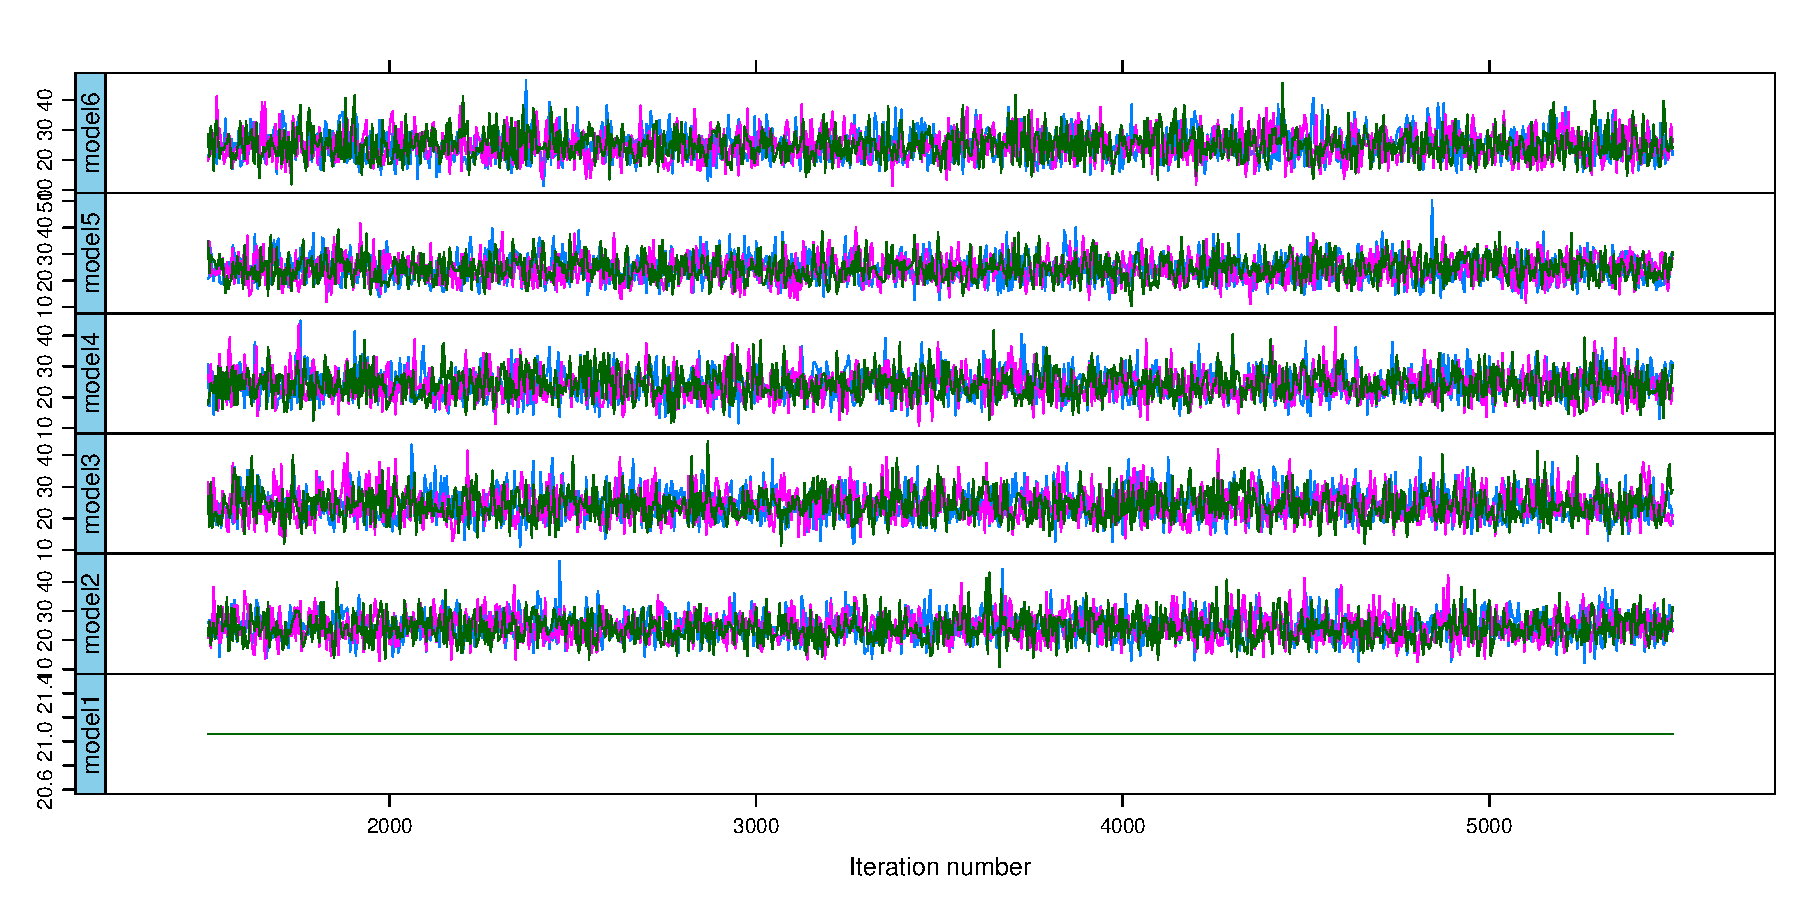
\includegraphics[width=1.0\linewidth]{../../R-codes/JAGS/plots/findmodel/Tracetotal3abn.PDF}
	\caption{Traces plot for category total of model 1 to model 6}
	\label{fig:tracetotal}
\end{figure}

\begin{figure}[!ht]
	\centering
	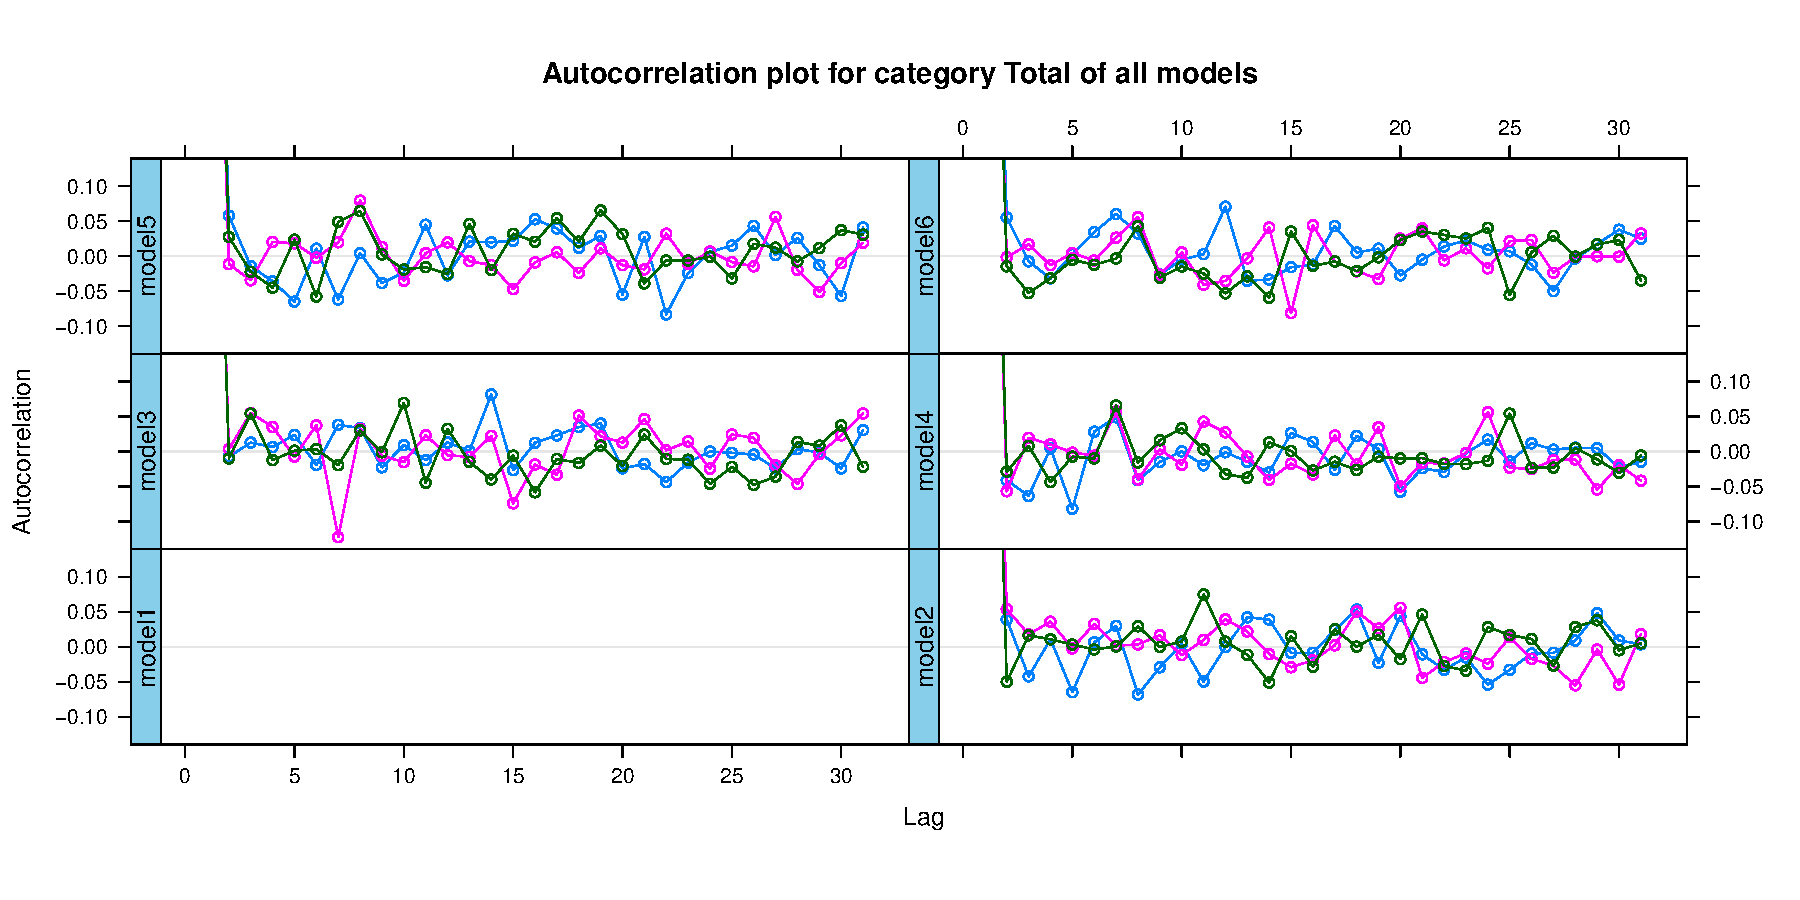
\includegraphics[width=1.0\linewidth]{../../R-codes/JAGS/plots/findmodel/Acftotal3abn.PDF}
	\caption{ACF plots for category total of model 1 to model 6}
	\label{fig:ACFtotal}
\end{figure}

Trace plots in figure~\ref{fig:tracetotal} allows a visual inspection of convergence at the top level of the hierarchy. The trace plot for model 1 is completely flat, suggesting that there is no mixing at all ( we have a fixed parameter), and trace plots for model 2 to 6 vary around the mean and do not show any trend, this suggest that our samples have mixed well and chains have converged. The Auto Correlation Function (ACF) plots presented in figure~\ref{fig:ACFtotal} gives no ACF for model 1; this indicates that model 1 gives no autocorrelation. ACF plots for model 2 to model 6 shows no signs of significant autocorrelation. 

\newpage %Z--------------------------------------------------------------

\begin{figure}[!ht]
	\centering
	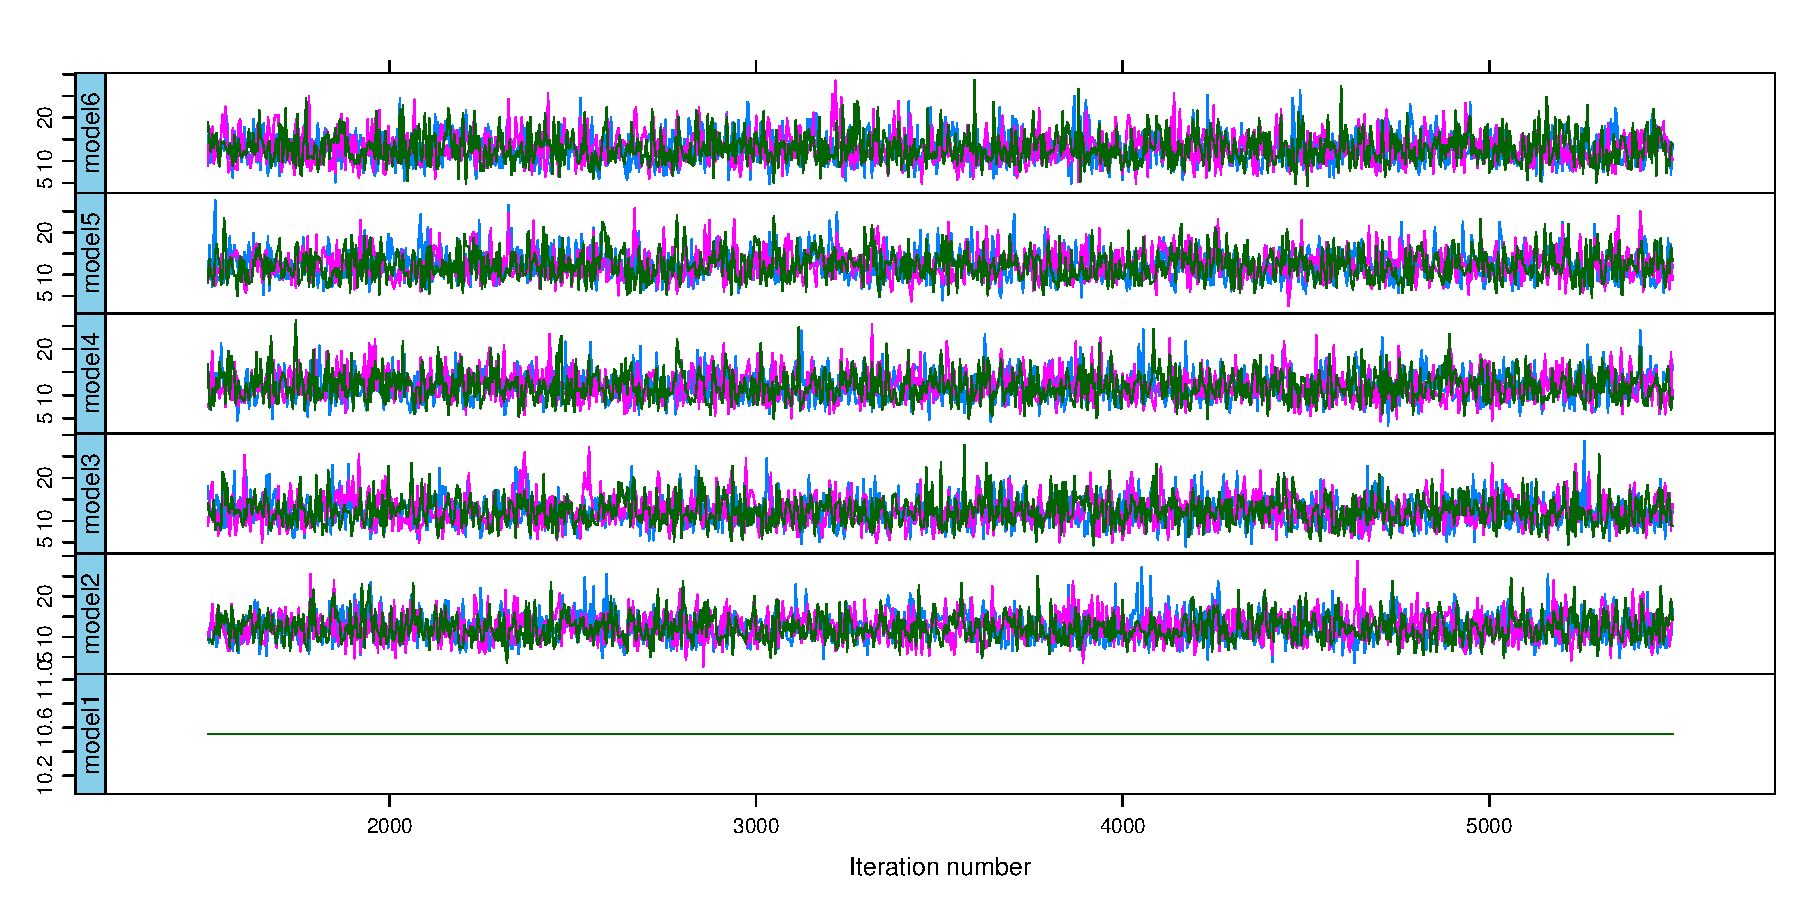
\includegraphics[width=1.0\linewidth]{../../R-codes/JAGS/plots/findmodel/TraceA3abn.PDF}
	\caption{Traces plot for category A of model 1 to model 6}
	\label{fig:traceA}
\end{figure}

\begin{figure}[!ht]
	\centering
	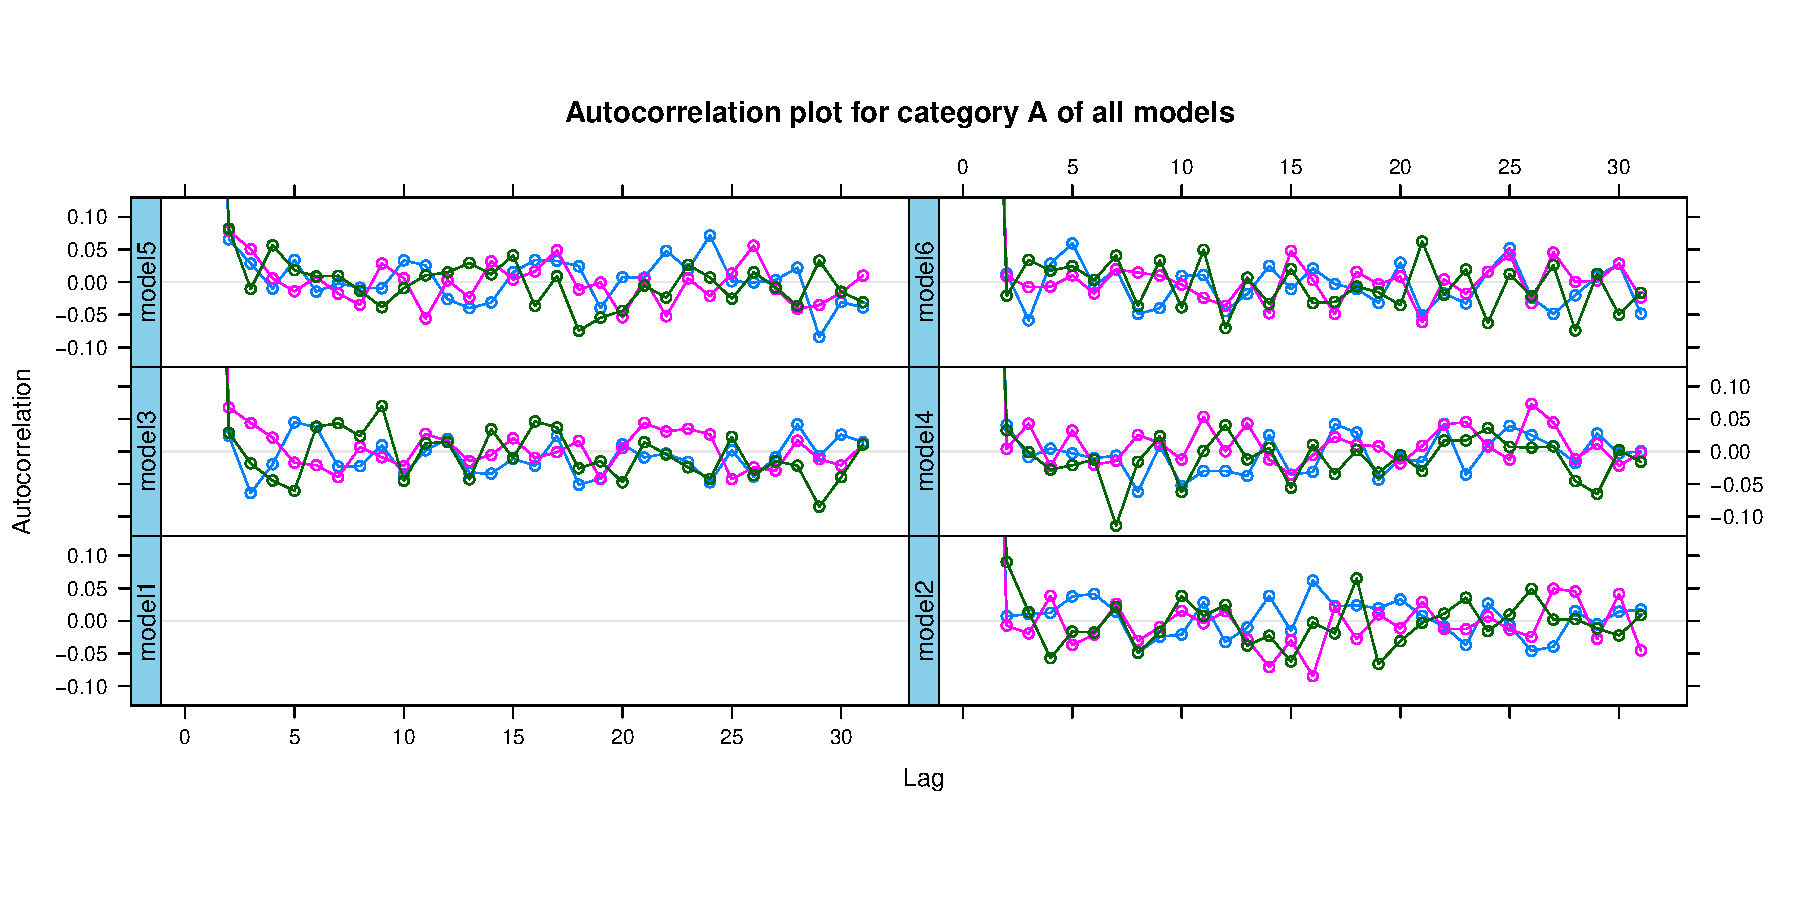
\includegraphics[width=1.0\linewidth]{../../R-codes/JAGS/plots/findmodel/AcfA3abn.PDF}
	\caption{ACFs plot for category A of model 1 to model 6}
	\label{fig:ACFA}
\end{figure}

Trace plots in figure~\ref{fig:traceA} allows a visual inspection of convergence at the second level of the hierarchy. The trace plot for model 1 is completely flat, suggesting that there is no mixing at all, and trace plots for model 2 to 6 vary around the mean and do not show any trend, this suggest that our samples have mixed well and chains have converged. The Auto Correlation Function (ACF) plots presented in figure~\ref{fig:ACFA} gives no ACF for model 1. Our observation indicates that model 1 gives no autocorrelation. ACF plots for model 2 to model 6 shows no signs of significant autocorrelation. 

\newpage %Z--------------------------------------------------------------

\begin{figure}[!ht]
	\centering
	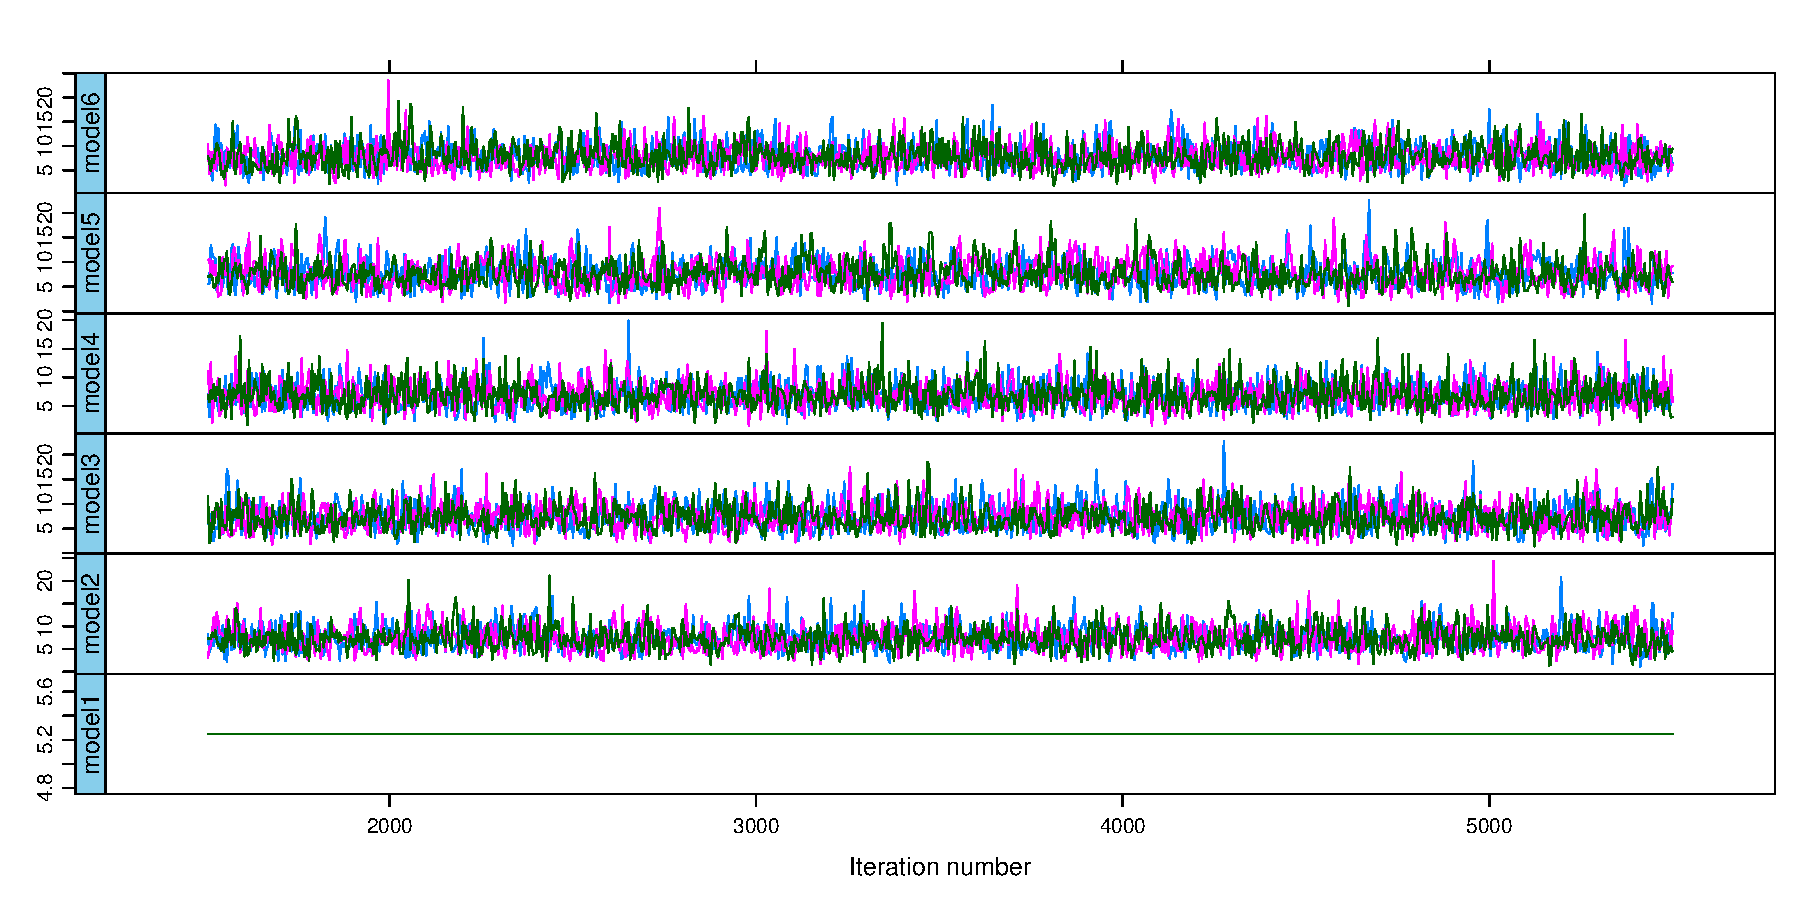
\includegraphics[width=1.0\linewidth]{../../R-codes/JAGS/plots/findmodel/TraceAA3abn.PDF}
	\caption{Traces plot for category AA of model 1 to model 6}
	\label{fig:traceAA}
\end{figure}

\begin{figure}[!ht]
	\centering
	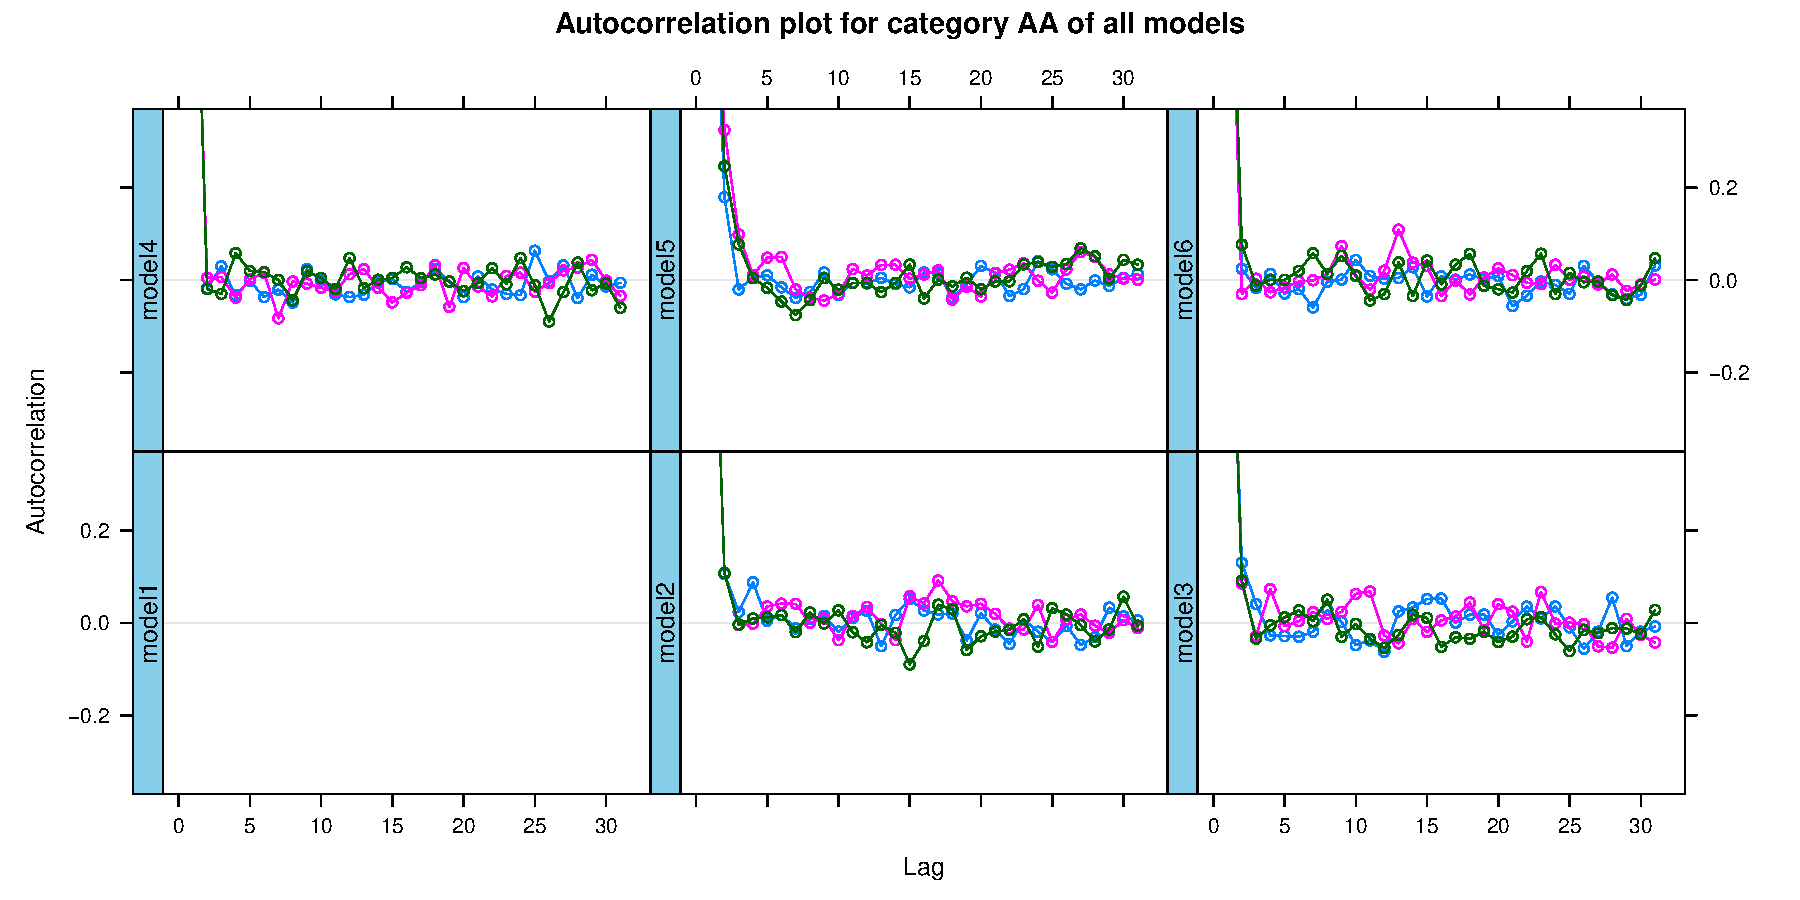
\includegraphics[width=1.0\linewidth]{../../R-codes/JAGS/plots/findmodel/AcfAA3abn.PDF}
	\caption{ACFs plot for category AA of model 1 to model 6}
	\label{fig:ACFAA}
\end{figure}

Trace plots in figure~\ref{fig:traceAA} allows a visual inspection of convergence at the second level of the hierarchy. The trace plot for model 1 is completely flat, suggesting that there is no mixing at all, and trace plots for model 2 to 6 vary around the mean and do not show any trend, this suggest that our samples have mixed well and chains have converged. The Auto Correlation Function (ACF) plots presented in figure~\ref{fig:ACFAA} gives no ACF for model 1; this indicates that model 1 gives no autocorrelation. ACF plots for model 2 to model 6 shows a weak sign of autocorrelation. 

\newpage

Considering trace plots and ACF plots results of all three hierarchical levels, we observe no strong correlation at all levels of hierarchy. However, there seems to be a slight increase in autocorrelation at lower levels of hierarchy. The is indicate that categories at lower hierarchy mixes slower compare to categories at the higher hierarchy.

\subsection{Discussion}

As expected, models that used weakly-informed priors had outperformed the model with non-informative prior, in terms of model goodness-of-fit, this highlighted the importance of assigning a prior distribution for Bayesian calculations and we should at least provide some distribution to our prior, even if it is just a flat uniform prior (which is also considered as a non-informative prior). Different hypothesised weakly-informed priors performed similarly, and we were unable to detect a significant difference between our priors from the DIC comparisons, and we did not observe significant differences in posterior distributions. If there is no evidence suggesting a prior is better than another prior, how do we decide which prior is preferable? The reasonable idea is that we should use the simplest prior, so complex priors such as the mixture prior and Laplace prior is out of the question. Especially for the case of Hierarchical Bayesian Model (HBM), we would want to build our HBM with the simplest prior as possible. Otherwise, our model would be extremely complex and hard to build. Hence, a Normal(1,0.3) prior is used for the rest of our simulations. A model with normal distributions is simple and suitable for observations with large samples as indicated by Central limit theorem (CLT) theorem. The essential idea is that weakly informative prior should contain enough information to regularize, this means that the prior should rule out unreasonable parameter values but is not so strong as to rule out values that might make sense. The might be other considerations as well, for example the Stan Development Team favour the lighter tails of a weakly informative prior with a Gaussian shape as the most robust default prior for it's accurate and fast statistical computation and ease of optimising the scale \citep{stan2018}, and \citet{gelman2006prior} suggested the usage of half-Cauchy prior distribution for observations with small values. 

\newpara

Another interesting find from this simulation is that uncertainty in Bayesian estimations will cause uncertainty in DIC results, and it is tough to confidently decide which model is the best if there is no substantial difference between the performance of models. Increasing the iteration number help a bit, but does not eliminate the problem and uncertainty still exists. A possible alternative to DIC is (Watanabe-Akaike information criteria), but it relies on a data partition that would cause difficulties with structured models \citep{gelman2014understanding}. Cross-validation could also work, but for Bayesian stats, it will be computationally expensive. Our results agree with conclusions from \citet{gelman2014understanding}, that predictive error comparisons (such as DIC) does work for highly dissimilar models, but have a weak performance for similar models, and sometimes it is challenging to draw significant conclusions.

%===============================================================================================================

\section{Simulation 2: Anomaly}

\subsection{Simulation setups}

In section 2.4, we present the results of the posterior distribution calculations for the synthesised data, with different increments of anomalies added on category AA on level 2 (leaf) of the hierarchy. The default setting for the data synthesis and anomaly addition process is applied for each scenario, with the addition of 0\%, 10\%, 25\%, 50\%, 100\%, 250\% and 500\% anomaly. An important note, the 25\% anomaly here meant an addition of 25\% of the count of category total ($\sum_i \mu_{i,t}$) on top of the hierarchy, not addition of 25\% on category AA.  

\subsection{Rsults}
\begin{table}[ht]
	\centering
	\begin{tabular}{crrrrrr}
		\hline
		Anomaly &&&&&&\\
		(\% of total) & Min. & 1st Qu. & Median & Mean & 3rd Qu. & Max. \\ 
		\hline
		0 & -0.466 & 0.188 & 0.437 & 0.545 & 0.955 & 1.556 \\ 
		10 & -1.910 & -0.693 & 0.876 & 1.144 & 1.894 & 6.640 \\ 
		25 & -6.274 & -3.079 & -1.966 & -1.984 & -0.658 & 1.825 \\ 
		50 & -4.352 & -1.185 & -0.038 & -0.385 & 0.823 & 2.420 \\ 
		100 & -5.074 & -1.096 & 0.323 & -0.383 & 1.194 & 1.873 \\ 
		250 & -1.813 & -1.657 & -0.917 & -0.181 & 0.546 & 3.681 \\ 
		500 & -4.416 & -1.678 & -0.613 & -0.875 & 0.430 & 1.401 \\ 
		\hline
	\end{tabular}
	\caption{DIC (with 1,000,000 iteration) comparisons between Independent Bayes model and Hierarchical Bayes model (HBM -IBM) for different anomalies sizes} 
	\label{tab:dicanomaly}
\end{table}

Table~\ref{tab:dicanomaly} gives the comparison of DIC distributions of Independent Bayesian Model (IBM) and Hierarchical Bayesian Model (HBM) for scenarios with different increments of anomaly added. For all scenarios, the mean and median value is mostly negative; the negative signals suggest that HBM seem to perform better than IBM, most of the time. Uncertainty in Bayesian estimations still exist and have impacts on the reliability of our DIC comparison, although we mostly see negative values for median and mean of the DIC difference distribution, the signal still shifts every time our JAGS model is re-run. Our observation suggests that although there might be a difference between IBM and HBM, it might not be a very big difference.  

\begin{table}[ht]
	\centering
	\begin{tabular}{rrrrrrrr}
		\hline
		& mean & sd & 2.5\% & 50\% & 97.5\% & Rhat & n.eff \\ 
		\hline
		Anomaly0 & 19.1481 & 4.2840 & 11.7152 & 18.8136 & 28.3845 & 1 & 3000 \\ 
		Anomaly10 & 21.4084 & 4.7272 & 13.1528 & 21.0041 & 31.6607 & 1 & 3000 \\ 
		Anomaly25 & 24.4356 & 4.9374 & 16.0687 & 24.0399 & 34.7248 & 1 & 2975 \\ 
		Anomaly50 & 30.2932 & 5.3613 & 20.8844 & 29.8973 & 41.9325 & 1 & 2912 \\ 
		Anomaly100 & 40.4338 & 6.1531 & 29.3330 & 40.0987 & 53.8314 & 1 & 2889 \\ 
		Anomaly250 & 71.9683 & 8.4372 & 56.5531 & 71.6763 & 89.4346 & 1 & 3000 \\ 
		Anomaly500 & 122.4365 & 10.7971 & 101.9952 & 122.2718 & 144.5457 & 1 & 3132 \\ 
		\hline
	\end{tabular}
	\caption{Posterior distributions of different models for Total, with different increments of added anomalies, and calculated with independent Bayes model} 
	\label{tab:pstanototal}
\end{table}

\begin{table}[ht]
	\centering
	\begin{tabular}{rrrrrrrr}
		\hline
		& mean & sd & 2.5\% & 50\% & 97.5\% & Rhat & n.eff \\ 
		\hline
		Anomaly0 & 19.3114 & 4.4361 & 11.5960 & 18.9555 & 28.9686 & 1 & 2934 \\ 
		Anomaly10 & 21.3883 & 4.5971 & 13.3033 & 21.1152 & 31.2900 & 1 & 2799 \\ 
		Anomaly25 & 24.3800 & 4.9083 & 15.8281 & 24.1057 & 34.9855 & 1 & 3000 \\ 
		Anomaly50 & 30.5664 & 5.4857 & 20.7071 & 30.2800 & 42.3242 & 1 & 2713 \\ 
		Anomaly100 & 40.5794 & 6.2480 & 29.1623 & 40.2459 & 53.0399 & 1 & 2704 \\ 
		Anomaly250 & 72.0177 & 8.2580 & 57.1126 & 71.8129 & 88.7105 & 1 & 2723 \\ 
		Anomaly500 & 121.9641 & 10.3188 & 102.7605 & 121.6646 & 142.4118 & 1 & 2173 \\ 
		\hline
	\end{tabular}
	\caption{Posterior distributions of different models for Total, with different increments of added anomalies, and calculated with Hierarchical Bayes model} 
	\label{tab:pstanototal2}
\end{table}

Table~\ref{tab:pstanototal} and table~\ref{tab:pstanototal2} gives the posterior distribution of the category total, with different increments of anomalies added, for IBM and HBM. There are differences between the mean and standard deviations of posteriors of IBM and HBM, but it is very small and very hard to tell. However, for HBM The number of Effective Sample Size (ESS) for HBM posteriors seem to be overall less than IBM posteriors, this suggests that values observed in total category on top of the hierarchy level for HBM are overall less independent than BM. As the size of the anomaly increases, the number of ESS tend to decrease. 

\newpage

\begin{table}[ht]
	\centering
	\begin{tabular}{rrrrrrrr}
		\hline
		& mean & sd & 2.5\% & 50\% & 97.5\% & Rhat & n.eff \\ 
		\hline
		Anomaly0 & 7.1758 & 2.7278 & 3.0586 & 6.7391 & 13.6749 & 1 & 2844 \\ 
		Anomaly10 & 9.3215 & 3.1367 & 4.1286 & 8.9552 & 16.3998 & 1 & 2630 \\ 
		Anomaly25 & 12.3410 & 3.5655 & 6.4488 & 11.9857 & 20.3604 & 1 & 3038 \\ 
		Anomaly50 & 18.4421 & 4.3162 & 10.8431 & 18.1170 & 27.7122 & 1 & 2839 \\ 
		Anomaly100 & 28.3032 & 5.3432 & 19.1588 & 27.8652 & 40.0187 & 1 & 3008 \\ 
		Anomaly250 & 58.6906 & 7.3628 & 45.1079 & 58.6335 & 73.7809 & 1 & 2118 \\ 
		Anomaly500 & 104.7585 & 9.5672 & 87.1657 & 104.5580 & 123.4846 & 1 & 2235 \\ 
		\hline
	\end{tabular}
	\caption{Posterior distributions of different models for A , with different increments of added anomalies, and calculated with Independent Bayes model} 
	\label{tab:pstanoA}
\end{table}

\begin{table}[ht]
	\centering
	\begin{tabular}{rrrrrrrr}
		\hline
		& mean & sd & 2.5\% & 50\% & 97.5\% & Rhat & n.eff \\ 
		\hline
		Anomaly0 & 7.1740 & 2.7263 & 2.8494 & 6.8467 & 13.2835 & 1 & 2559 \\ 
		Anomaly10 & 9.1731 & 3.0292 & 4.1612 & 8.8307 & 15.8837 & 1 & 2961\\ 
		Anomaly25 & 12.4274 & 3.6049 & 6.3125 & 12.0656 & 20.2620 & 1 & 2703 \\ 
		Anomaly50 & 18.5048 & 4.3162 & 10.9271 & 18.2437 & 28.0090 & 1 & 2580 \\ 
		Anomaly100 & 28.6123 & 5.2341 & 19.2090 & 28.1992 & 39.9182 & 1 & 2370 \\ 
		Anomaly250 & 59.6236 & 7.2375 & 46.4370 & 59.4535 & 74.8256 & 1 & 1940 \\ 
		Anomaly500 & 107.9043 & 9.7689 & 89.7498 & 107.4554 & 129.0404 & 1 & 1338 \\ 
		\hline
	\end{tabular}
	\caption{Posterior distributions of different models for A , with different increments of added anomalies, and calculated with Hierarchical Bayes model} 
	\label{tab:pstanoA2}
\end{table}

Table~\ref{tab:pstanoA} and table~\ref{tab:pstanoA2} gives the posterior distribution of the category A, with different increments of anomalies added, for IBM and HBM. There are also differences between the mean and standard deviations of posteriors of IBM and HBM, but it is also very small and very hard to tell. The number of ESS for HBM posteriors seem to be overall less than IBM posteriors. Our observation suggests that values observed in A category on second of the hierarchy level for HBM are overall less independent than BM. As the size of the anomaly increases, the number of ESS tend to decrease. 

\newpage

\begin{table}[ht]
	\centering
	\begin{tabular}{rrrrrrrr}
		\hline
		& mean & sd & 2.5\% & 50\% & 97.5\% & Rhat & n.eff \\ 
		\hline
		Anomaly0 & 2.3062 & 1.4859 & 0.4009 & 2.0034 & 6.0143 & 1 & 2401 \\ 
		Anomaly10 & 4.2976 & 2.1384 & 1.2137 & 3.8992 & 9.5420 & 1 & 2461 \\ 
		Anomaly25 & 7.4243 & 2.8041 & 2.8709 & 7.0744 & 13.8003 & 1 & 2214\\ 
		Anomaly50 & 13.3455 & 3.5920 & 7.3160 & 13.0175 & 21.0238 & 1 & 2428 \\ 
		Anomaly100 & 22.4374 & 4.5194 & 14.6914 & 22.0898 & 31.9623 & 1 & 2029 \\ 
		Anomaly250 & 48.8502 & 6.1544 & 37.2238 & 48.5964 & 61.2842 & 1 & 1568 \\ 
		Anomaly500 & 100.5322 & 11.0472 & 79.0267 & 100.3259 & 122.1376 & 1 & 1115 \\ 
		\hline
	\end{tabular}
	\caption{Posterior distributions of different models for AA, with different increments of added anomalies, and calculated with Independent Bayes model} 
	\label{tab:pstanoAA}
\end{table}

\begin{table}[ht]
	\centering
	\begin{tabular}{rrrrrrrr}
		\hline
		& mean & sd & 2.5\% & 50\% & 97.5\% & Rhat & n.eff \\ 
		\hline
		Anomaly0 & 2.1538 & 1.4960 & 0.3505 & 1.7838 & 6.1010 & 1 & 2073 \\ 
		Anomaly10 & 4.3301 & 2.1448 & 1.1920 & 3.9651 & 9.5508 & 1 & 2046 \\ 
		Anomaly25 & 7.6847 & 2.8131 & 3.0945 & 7.3379 & 13.8861 & 1 & 2149 \\ 
		Anomaly50 & 13.6061 & 3.6369 & 7.2589 & 13.3337 & 21.4732 & 1 & 2054 \\ 
		Anomaly100 & 23.0253 & 4.5067 & 14.9764 & 22.7288 & 32.6668 & 1 & 1679 \\ 
		Anomaly250 & 51.9695 & 6.3876 & 40.2516 & 51.8076 & 65.5484 & 1 & 951 \\ 
		Anomaly500 & 96.0807 & 9.1704 & 79.5825 & 95.8225 & 115.7111 & 1& 951 \\ 
		\hline
	\end{tabular}
	\caption{Posterior distributions of different models for AA, with different increments of added anomalies, and calculated with Hierarchical Bayes model} 
	\label{tab:pstanoAA2}
\end{table}

Table~\ref{tab:pstanoAA} and table~\ref{tab:pstanoAA2} gives the posterior distribution of the category AA, with different increments of anomalies added, for IBM and HBM. There are also differences between the mean and standard deviations of posteriors of IBM and HBM, but it is also very small and very hard to tell. The number of ESS for HBM posteriors seem to be overall less than IBM posteriors. Our observation suggests that values observed in the AA category on the bottom of the hierarchy level for HBM are overall less independent than IBM. As the size of the anomaly increases, the number of ESS tend to decrease. 

\newpage

Overall, we make a similar observation on posterior distributions for categories on different levels of the hierarchy, for scenarios with different increments of anomalies added. Increase of size of anomalies will result in higher mean and standard deviation, and a smaller ESS overall, for categories on all levels of the hierarchy. Differences in posterior distributions of HBM and IBM seem to exist, but it is tiny and is likely to be masked by the noise from uncertainties in Bayesian estimates. However, the variability in differences seem to be greater for categories at a lower level of the hierarchy, i.e. there is a difference of 0.47, 2.74, and 4.49 in IBM and HBM means of 500\% anomaly. Our observation suggests that the HBM model have a greater difference in performance, for observations in lower levels of hierarchy. The ESS also has a significant overall decrease for our posterior results in lower levels of hierarchy, suggesting that IBM greatly reduce the independence of our results. 
\newpara

\underline{\textbf{Notes on heat-maps}}

\newpara

As mentioned in section~\ref{chap:anom}, a hypothetical value called capacity ($k$) is used to set up the threshold for what we believe to be values that reflect anomalous events. The basic idea is that $k$ is a measure of hospital capacity, once the capacity is reached, congestion will definitely occur. The threshold is simply the inverse of $k$, so a $k$ of 0.8 would mean that the threshold is set to be 1.25 times the expected mean arrival $\mu$. A larger $k$ stands for higher capacity and would result in a smaller multiplication factor for $\mu$ for the threshold value. Vice versa, a smaller $k$ stands for lower capacity and would result in a larger multiplication factor for $\mu$ for the threshold value. The idea makes sense because when hospitals operate at high capacity, it will not take much to overfill their capacity. However, when a hospital is operating at a lower capacity, there is a large buffer-zone, and it would take a sizeable abnormal arrival to fill the capacity.

\newpara

A threshold is used to calculate the area of the posterior distribution that falls under the distribution, that exceeds the threshold. The Threshold gives a single measure of posterior probability $\theta$ that is over the threshold, higher the $\theta$ more of the posterior probability will fall over the threshold, and smaller the $\theta$ less posterior probability will fall under the threshold. A $\theta$ close to 0.50 would suggest that our median value of posterior probability is falling right on the threshold. Larger the $\theta$ more confident we have for the occurrence of an anomaly. $\theta$ from our models and scenarios are then tabulated with different increments of $k$ and presented in A 10 level colour-coded heat map. The colour of the heat map is in the classic red and blue spectrum, with red indicating a larger $\theta$ and a higher probability of observing an anomaly, and blue indicating a smaller $\theta$ and a lower probability of observing an anomaly. 

%-----------------------------------------------------------------------------------------
\newpage

\begin{figure}[!h]
	\centering
	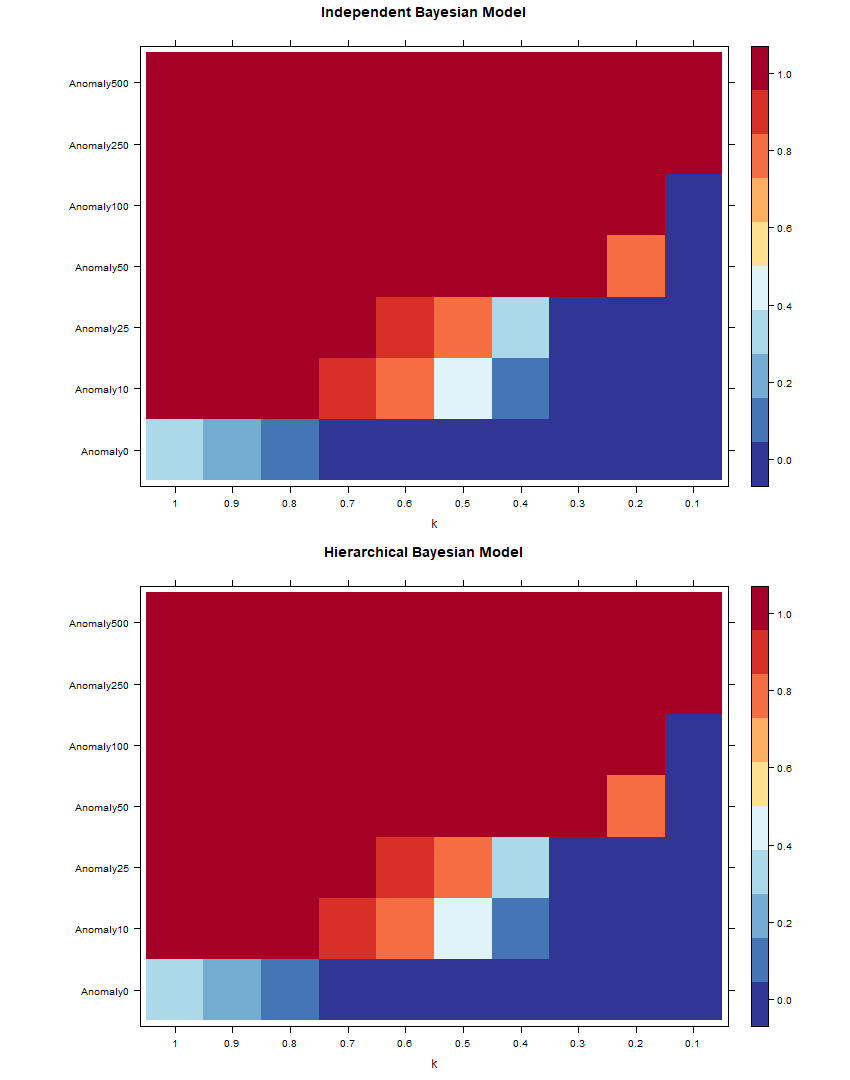
\includegraphics[width=1\linewidth]{../../R-codes/JAGS/plots/sim1/heattotal}
	\caption{Heat-map of anomaly alarms for different size of anomaly under different k values, of IBM and HBM, at category total.}
	\label{fig:heattotalab}
\end{figure}

\newpage

\begin{figure}[!h]
	\centering
	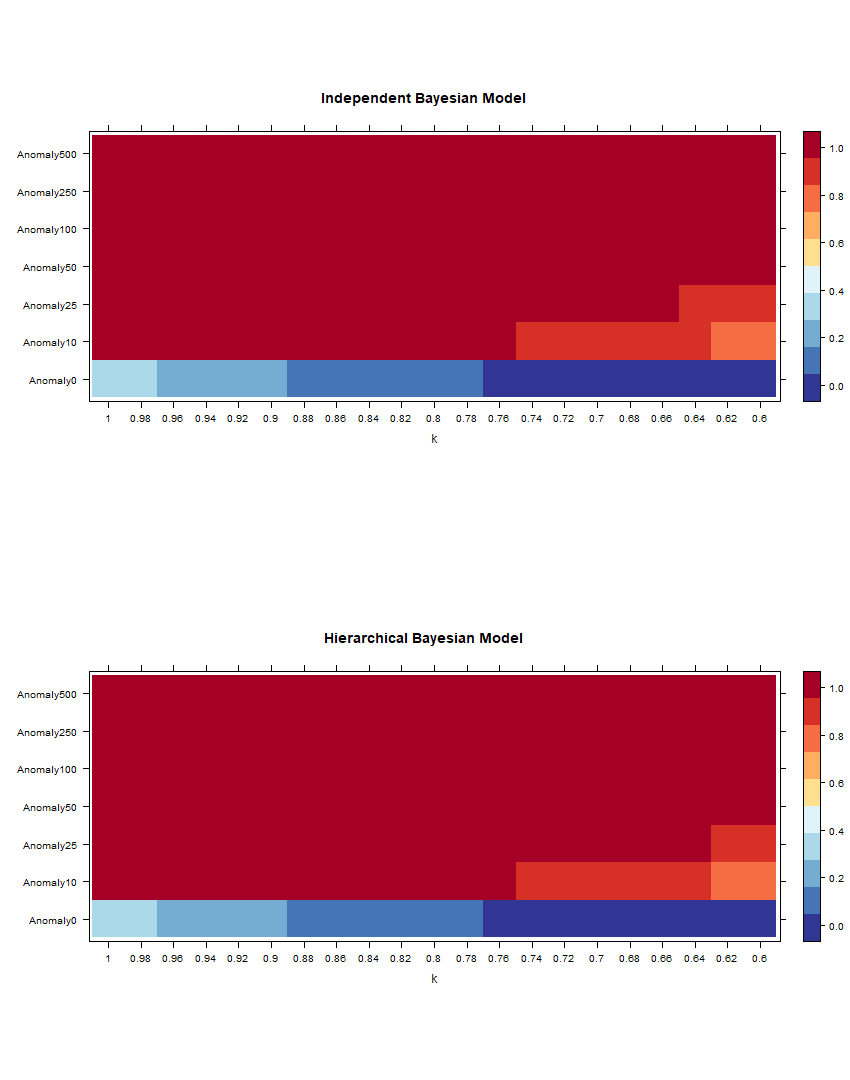
\includegraphics[width=1\linewidth]{../../R-codes/JAGS/plots/sim1/heattotal2}
	\caption{Heat-map of anomaly alarms for different size of anomaly under different k values, of IBM and HBM zoomed in at k values of 0.6 to 1, at category total.}
	\label{fig:heattotalab2}
\end{figure}

\newpage

The heat-map in figure~\ref{fig:heattotalab} presents the anomaly signals of category total for different increments of anomaly added, with IBM and HBM, against different increments of $k$. Strong anomaly signals (in red) tend to appear toward the top left corner of our heap-map, this indicated that signals of anomaly tend to increase in strength with greater anomaly and higher capacity $k$. Zooming in at looking at $k$ values from 0.6 to 1 in figure~\ref{fig:heattotalab2}, we observe a minimal difference in anomaly detection rate between IBM and HBM for category total. Our observation suggests that the difference between anomaly detection rate is small or close to none for IBM and HBM, on the top level of the hierarchy, for all sizes of the anomaly, in a simulated setting with each category generated independently. 

%-----------------------------------------------------------------------------------------
\newpage

\begin{figure}[!h]
	\centering
	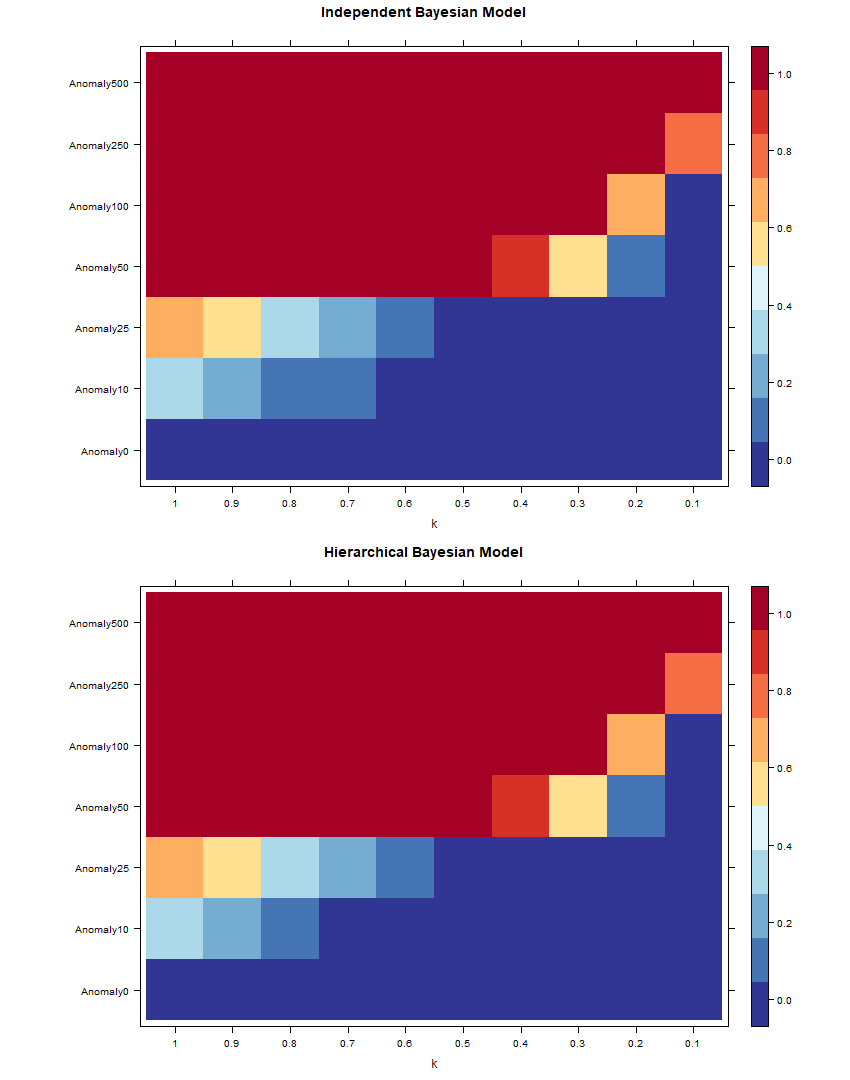
\includegraphics[width=1\linewidth]{../../R-codes/JAGS/plots/sim1/heatA}
	\caption{Heat-map of anomaly alarms for different size of anomaly under different k values, of IBM and HBM, at category A.}
	\label{fig:heatAab}
\end{figure}

\newpage

\begin{figure}[!h]
	\centering
	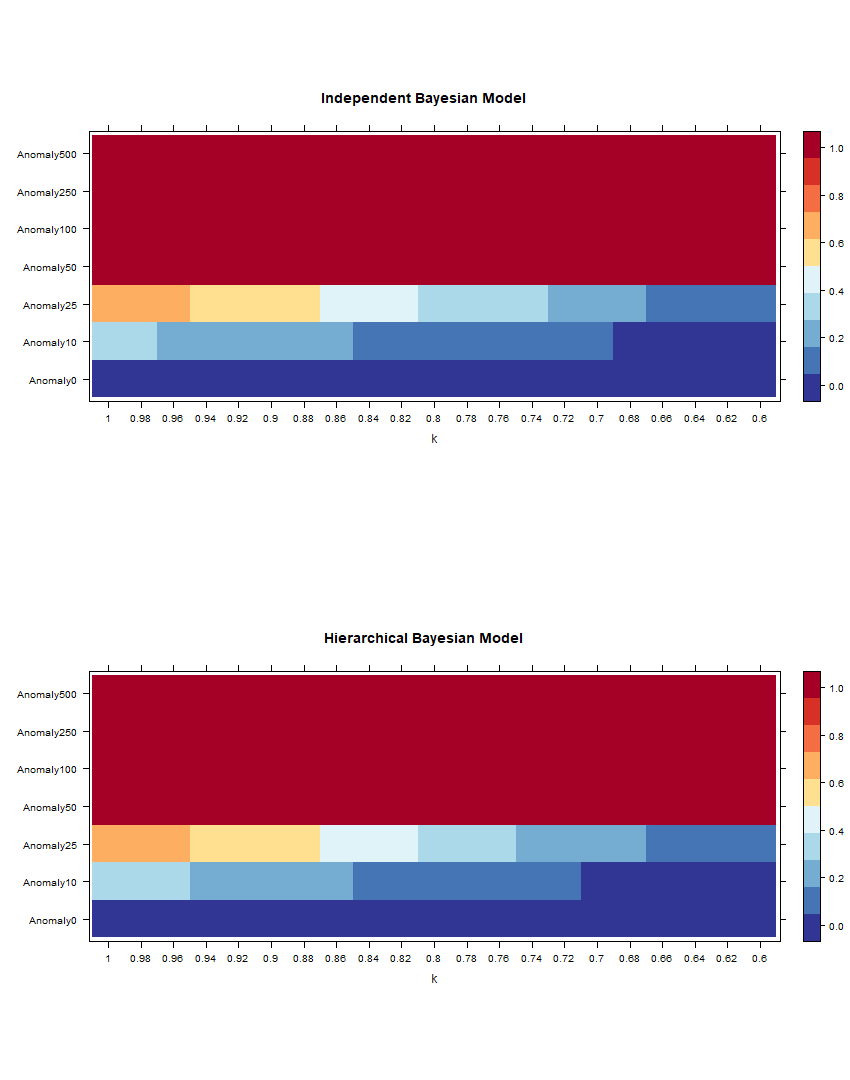
\includegraphics[width=1\linewidth]{../../R-codes/JAGS/plots/sim1/heatA2}
	\caption{Heat-map of anomaly alarms for different size of anomaly under different k values, of IBM and HBM zoomed in at k values of 0.6 to 1, at category A.}
	\label{fig:heatA2ab}
\end{figure}

\newpage

The heat-map in figure~\ref{fig:heatAab} presents the anomaly signals of category A for different increments of anomaly added, with IBM and HBM, against different increments of $k$. Strong anomaly signals (in red) tend to appear toward the top left corner of our heap-map, this indicated that signals of anomaly tend to increase in strength with greater anomaly and higher capacity $k$.Zooming in at looking at k values from 0.6 to 1 in figure~\ref{fig:heatA2ab}, we observe a minimal difference in anomaly detection rate between IBM and HBM for category A. Our observation suggests that the difference between anomaly detection rate is small or close to none for IBM and HBM, on level 2 of the hierarchy, for all sizes of anomaly, in a simulated setting with each category generated independently. 

%-----------------------------------------------------------------------------------------

\newpage

\begin{figure}[!h]
	\centering
	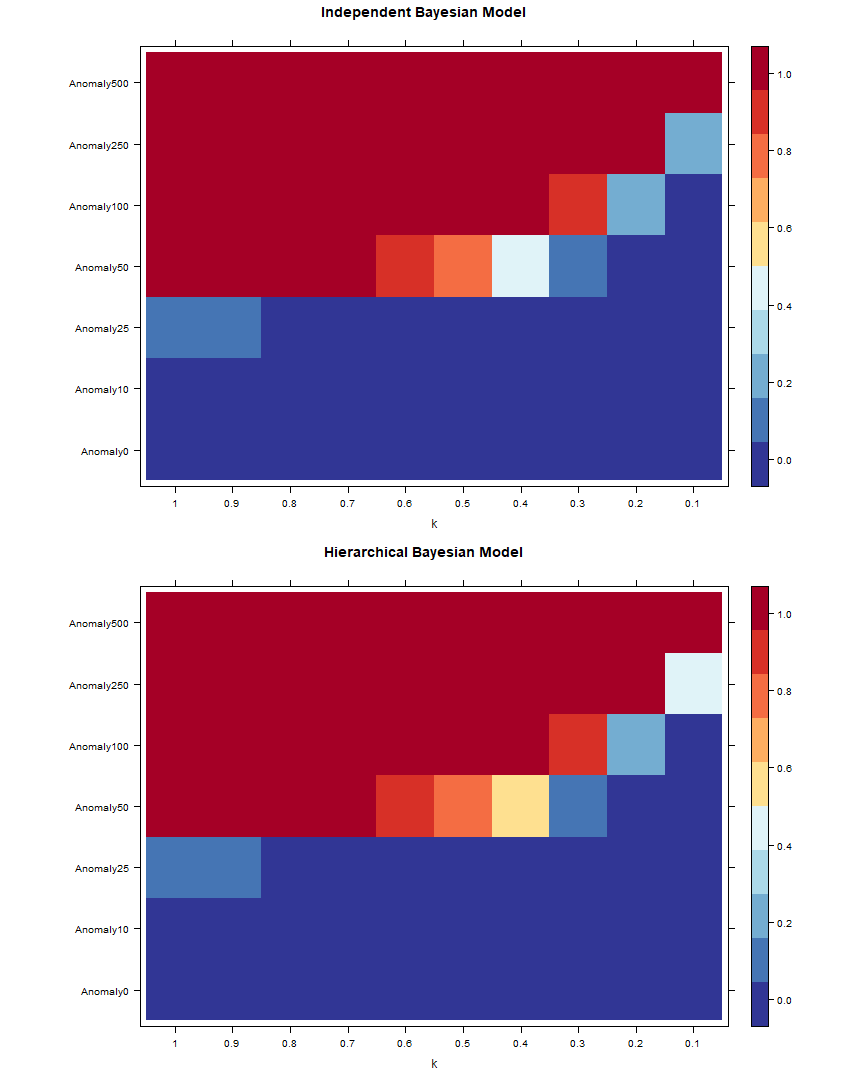
\includegraphics[width=1\linewidth]{../../R-codes/JAGS/plots/sim1/heatAA}
	\caption{Heat-map of anomaly alarms for different size of anomaly under different k values, of IBM and HBM, at category AA.}
	\label{fig:heatAAab}
\end{figure}

\newpage

\begin{figure}[!h]
	\centering
	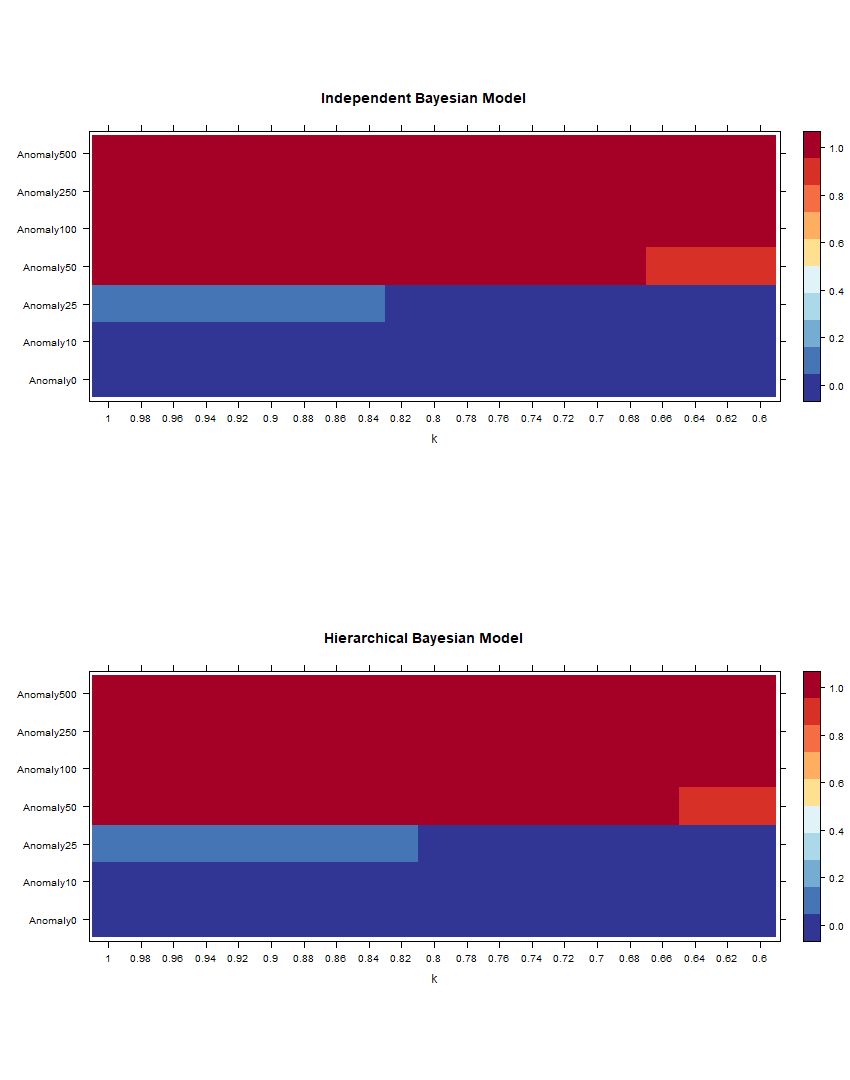
\includegraphics[width=1\linewidth]{../../R-codes/JAGS/plots/sim1/heatAA2}
	\caption{Heat-map of anomaly alarms for different size of anomaly under different k values, of IBM and HBM zoomed in at k values of 0.6 to 1, at category AA.}
	\label{fig:heatAA2ab}
\end{figure}

\newpage
The heat-map in figure~\ref{fig:heatAAab} presents the anomaly signals of category AA for different increments of anomaly added, with IBM and HBM, against different increments of $k$. Strong anomaly signals (in red) tend to appear toward the top left corner of our heap-map, this indicated that signals of anomaly tend to increase in strength with greater anomaly and greater capacity $k$. Zooming in at looking at k values from 0.6 to 1 in figure~\ref{fig:heatAA2ab}, we observe a minimal difference in anomaly detection rate between IBM and HBM for category AA. Our observation suggests that the difference between anomaly detection rate is small or close to none for IBM and HBM, on the bottom of the hierarchy, for all sizes of the anomaly, in a simulated setting with each category generated independently. 

\newpara

Comparing between levels of hierarchies, we observe that for all levels of hierarchy, strong anomaly signals (in red) tend to appear toward the top left corner of our heap-map, confirming the fact that signals of anomaly tend to increase in strength with greater anomaly and higher capacity $k$, for all levels of hierarchy. For all levels of hierarchy, We observe powerful red signals for scenarios with 50\% and more anomalies added, and very weak signals for the case of no anomaly, 10\% anomaly and 25\% anomaly. The overall signals for higher hierarchies tend to be stronger than overall signals in lower hierarchies. 


\subsection{Discussion}

Our DIC results suggest that compared to IBM, HBM gives better goodness of fit and is the better model, for scenarios with different increments of anomalies added to a category at the bottom level of the hierarchy, this provided more evidence that suggests that HBM are superior compared to IBM. Although our DIC comparisons result varies every time we re-ran our JAGS models, the observation appears most of the time, and we have some evidence to back our claim. The finding is consistent with the finds in  \citet{gelman2006multilevel}, that hierarchical models tend to give a better prediction compare to no-pooling (independent) models in all levels. Although our DIC result suggests that HBM gives a different and better posterior distribution, it is kind of hard to tell the differences between posterior distributions for IBM and HBM with all the noise present, and this reduced out confidence to our claim. To rule out the noise from uncertainties in Bayesian posterior is a complex and calculation-intensive process and are out of our scope.

\newpara

As the size of the anomaly increases, the number of ESS tend to decrease. The observation is due to the fact that a more substantial increase in anomaly results in a more substantial, more influential constant change in observed values, that produces a strong autocorrelation relationship and this will reduce the independence of the values, this is also the reason why the standard deviation of posterior also tend to increase as we increase the size of anomalies. The reasoning also applies to hierarchical levels, due to the aggregation constraint values at each level tend to increase, and sample distributions tend to approximate towards normal. So when we are dealing with hierarchical datasets, we must take into account the hierarchical structure, there are significant statistical information within the hierarchy and disregarding the hierarchical structure would significantly reduce the power of our models. A tell-tale sign that IBM had disregarded information about the hierarchical structure is that posterior distributions of IBM tend to have a greater ESS compare to HBM, information between levels often translate into correlations, and without this information, the posterior results in each category would be more independent have a greater ESS. The loss of information becomes more apparent for lower levels of hierarchy; this is because values of a category at a lower level of hierarchy often influenced by an increasing number of more population-level parameter. 

\newpara

With our posterior distributions, we were able to set up a theoretical threshold and made attempts to detect anomalies. Signals of anomaly tend to increase in strength with larger anomalies and higher capacity ($k$), for all levels of hierarchy. Our observations made sense; it is easier to detect larger anomalies because the posterior will be larger and more likely to fall over the threshold. Also, as capacity increase, the average expected value closer to the threshold, and it becomes easier a higher than expected value to go over the threshold. I.e. for a capacity of 80\%, we need a positive anomaly 1.25 times the expected value to meet the threshold, for a capacity of 40\%, we need a positive anomaly 2.5 times the expected value to meet the threshold. Relating to the idea of congestion mentioned in the previous section,  for a hospital to decrease the likelihood of encountering congestion, we would need to decrease the operation capacity of its facilities. Operating at a high capacity may save resource, but is the downside worth it? Did the policymaker take in an account of adverse effects such as doctors getting burnout and an increasing likelihood of congestion, and does the risk out weight the benefit? 

\newpage

\section{Simulation 3: Structure }

\subsection{Simulation setups }

In section 2.5, we present the results of the posterior distribution calculations for the synthesised data, with same 10\% anomaly added on category AA on level 2 (leaf) of the hierarchy, but for hierarchies with a different structure. Most of the hierarchical structure is controlled to be the same, except for the branching at category A. We create 12 scenarios with category A branching into 1 to 12 subgroups equal in size. So for branch = 1,  category A will branch into one subcategory AA, category AA will contain 100\% of the size of the category. For branch = 3, category A will branch into three subcategory AA, AB and AC, category AA, AB and AC will each contain 33\% of the size of category A. 

\subsection{Results}

\begin{table}[ht]
	\centering
	\begin{tabular}{rrrrrrr}
		\hline
		Branch & Min. & 1st Qu. & Median & Mean & 3rd Qu. & Max. \\ 
		\hline
		1 & -7.033 & -1.960 & -0.809 & -1.527 & 0.294 & 1.172 \\ 
		2 & -4.435 & -2.722 & -0.994 & -0.591 & 0.214 & 6.308 \\ 
		3 & -2.710 & -1.013 & 0.554 & 0.521 & 1.440 & 4.575 \\ 
		4 & -3.418 & -0.451 & 0.370 & 0.305 & 1.422 & 3.356 \\ 
		5 & -2.715 & -1.447 & -1.065 & -0.318 & 1.022 & 2.791 \\ 
		6 & -3.082 & -0.733 & -0.129 & 0.121 & 1.042 & 4.216 \\ 
		7 & -4.280 & -2.843 & -1.286 & -1.581 & -0.213 & 0.790 \\ 
		8 & -4.349 & -2.215 & -0.967 & -0.422 & 1.065 & 7.971 \\ 
		9 & -4.931 & -1.649 & -0.335 & -0.303 & 1.014 & 4.038 \\ 
		10 & -5.247 & -1.578 & -0.234 & -0.668 & 0.618 & 3.247 \\ 
		11 & -2.597 & -1.126 & 1.002 & 0.466 & 1.655 & 3.751 \\ 
		12 & -3.340 & -1.786 & -0.102 & 0.223 & 1.838 & 4.623 \\ 
		\hline
	\end{tabular}
	\caption{DIC comparisons for branching number at A} 
	\label{tab:dicanomaly2}
\end{table}

Table~\ref{tab:dicanomaly2} gives the comparison of DIC distributions of Independent Bayesian Model (IBM) and Hierarchical Bayesian Model (HBM) for scenarios with a different hierarchical structure. For all scenarios, the mean and median value is mostly negative; the negative signals suggest that HBM seem to perform better than IBM, most of the time. Uncertainty in Bayesian estimations still exist and have impacts on the reliability of our DIC comparison, although we mostly see negative values for median and mean of the DIC difference distribution, the signal still shifts every time our JAGS model is re-run. Our observation suggests that although there might be a difference between IBM and HBM, it might not be a very big difference. 

\newpage 

\begin{table}[!t]
	\centering
	\begin{tabular}{rrrrrrrr}
		\hline
		Branch & mean & sd & 2.5\% & 50\% & 97.5\% & Rhat & n.eff \\ 
		\hline
		1 & 21.2367 & 4.7008 & 12.9239 & 20.9013 & 31.1209 & 1 & 2787 \\ 
		2 & 21.4198 & 4.6439 & 13.5516 & 20.9515 & 31.6895 & 1 & 2904 \\ 
		3 & 30.4154 & 5.6673 & 20.1950 & 30.2022 & 42.1275 & 1 & 2877 \\ 
		4 & 13.1540 & 3.5731 & 6.9948 & 12.7660 & 21.1359 & 1 & 3000 \\ 
		5 & 26.4296 & 5.0584 & 17.2806 & 26.1034 & 37.3137 & 1 & 2815 \\ 
		6 & 22.3157 & 4.7457 & 14.0816 & 22.0346 & 32.1219 & 1 & 2881 \\ 
		7 & 17.2269 & 4.1264 & 10.2189 & 16.7961 & 26.4545 & 1 & 2587 \\ 
		8 & 19.1497 & 4.3697 & 11.4783 & 18.8391 & 28.4958 & 1 & 3000\\ 
		9 & 27.4028 & 5.2818 & 18.0539 & 26.9926 & 38.6413 & 1 & 2854 \\ 
		10 & 18.2805 & 4.2982 & 10.6334 & 18.0157 & 27.3239 & 1 & 3028 \\ 
		11 & 22.2082 & 4.7100 & 13.9406 & 21.8632 & 32.7639 & 1 & 3000 \\ 
		12 & 23.2141 & 4.8762 & 14.6652 & 22.8895 & 33.4077 & 1 & 3090 \\ 
		\hline
	\end{tabular}
	\caption{Posterior distributions of different models for Total, with different brnch number at A, and calculated with Independent Bayes model} 
	\label{tab:pstprototal}
\end{table}

\begin{table}[!h]
	\centering
	\begin{tabular}{rrrrrrrr}
		\hline
		Branch & mean & sd & 2.5\% & 50\% & 97.5\% & Rhat & n.eff \\ 
		\hline
		1 & 21.1342 & 4.6356 & 13.0372 & 20.8723 & 31.0156 & 1 & 2899 \\ 
		2 & 21.4399 & 4.6658 & 13.3765 & 21.0743 & 31.3564 & 1 & 2888 \\ 
		3 & 30.4796 & 5.5918 & 20.4537 & 30.1087 & 42.6573 & 1 & 3069 \\ 
		4 & 13.0428 & 3.6218 & 6.9370 & 12.7050 & 21.1728 & 1 & 2798 \\ 
		5 & 26.4792 & 5.0783 & 17.5450 & 26.1769 & 37.5123 & 1 & 2903 \\ 
		6 & 22.5513 & 4.7242 & 14.3816 & 22.2968 & 32.5958 & 1 & 3000 \\ 
		7 & 17.2175 & 4.1172 & 9.9473 & 16.9176 & 25.9870 & 1 & 3000 \\ 
		8 & 19.2860 & 4.3666 & 11.7869 & 19.0001 & 28.9699 & 1 & 2712 \\ 
		9 & 27.4363 & 5.2930 & 18.1801 & 27.1123 & 38.8600 & 1 & 2719 \\ 
		10 & 18.3153 & 4.2436 & 10.9404 & 18.0915 & 27.1782 & 1 & 2961 \\ 
		11 & 22.2699 & 4.7638 & 13.7242 & 21.8257 & 32.6838 & 1 & 3000 \\ 
		12 & 23.3112 & 4.9101 & 14.5832 & 22.9914 & 33.6660 & 1 & 3006 \\ 
		\hline
	\end{tabular}
	\caption{Posterior distributions of different models for Total, with different branch number at A, and calculated with Hierarchical Bayes model} 
	\label{tab:pstprototalh}
\end{table}

Table~\ref{tab:pstprototal} and table~\ref{tab:pstprototalh} gives the posterior distribution of the category total, for scenarios with different hierarchical structure. Our results show a large variability between posterior distribution for category total at the top of the structure hierarchy, but there are no obvious trends for different hierarchical structures and IBM and HBM models in any of the values due to the presence of noise. 

\newpage

\begin{table}[!t]
	\centering
	\begin{tabular}{rrrrrrrr}
		\hline
		Branch & mean & sd & 2.5\% & 50\% & 97.5\% & Rhat & n.eff \\ 
		\hline
		1 & 10.2222 & 3.2257 & 4.9491 & 9.9313 & 17.3630 & 1 & 3000 \\ 
		2 & 7.2101 & 2.5820 & 3.0653 & 6.9089 & 13.0457 & 1& 3135 \\ 
		3 & 13.3965 & 3.5903 & 7.1940 & 13.0422 & 21.4547 & 1 & 2843 \\ 
		4 & 5.2344 & 2.2966 & 1.7544 & 4.9212 & 10.8095 & 1 & 2659 \\ 
		5 & 12.2653 & 3.5442 & 6.3801 & 11.9468 & 20.0809 & 1 & 2831 \\ 
		6 & 12.4534 & 3.5617 & 6.4566 & 12.0511 & 20.3078 & 1 & 2826 \\ 
		7 & 11.3345 & 3.3140 & 5.6904 & 11.0780 & 18.6164 & 1 & 2763 \\ 
		8 & 11.3301 & 3.4455 & 5.6405 & 10.9504 & 18.8542 & 1 & 3000 \\ 
		9 & 15.2998 & 3.9278 & 8.5925 & 15.0144 & 24.1089 & 1 & 3000\\ 
		10 & 10.2282 & 3.2404 & 4.9712 & 9.8590 & 17.4283 & 1 & 2719 \\ 
		11 & 12.2384 & 3.5230 & 6.2765 & 11.9505 & 19.9642 & 1 & 3000 \\ 
		12 & 16.2605 & 4.1472 & 9.1019 & 15.9211 & 25.5411 & 1 & 2614 \\ 
		\hline
	\end{tabular}
	\caption{Posterior distributions of different models for A , with different branch number at A, and calculated with independent Bayes model} 
	\label{tab:pstproA}
\end{table}

\begin{table}[!h]
	\centering
	\begin{tabular}{rrrrrrrr}
		\hline
		Branch & mean & sd & 2.5\% & 50\% & 97.5\% & Rhat & n.eff \\ 
		\hline
		1 & 10.3658 & 3.2745 & 4.9563 & 9.9946 & 17.5591 & 1 & 2480 \\ 
		2 & 7.1699 & 2.7092 & 2.8318 & 6.7969 & 13.3853 & 1 & 2763 \\ 
		3 & 13.5106 & 3.6263 & 7.2349 & 13.2756 & 21.5433 & 1 & 2721 \\ 
		4 & 4.9821 & 2.1601 & 1.7617 & 4.6571 & 9.9815 & 1 & 2848 \\ 
		5 & 12.2966 & 3.5260 & 6.2470 & 11.9827 & 20.1420 & 1 & 2691 \\ 
		6 & 11.9993 & 3.3669 & 6.1917 & 11.7362 & 19.3448 & 1 & 2515 \\ 
		7 & 11.1468 & 3.3194 & 5.5362 & 10.8140 & 18.2800 & 1 & 2791 \\ 
		8 & 10.9205 & 3.2059 & 5.5478 & 10.6286 & 17.9246 & 1 & 2596 \\ 
		9 & 15.1743 & 3.7615 & 8.6417 & 14.8581 & 23.3316 & 1 & 2371 \\ 
		10 & 9.4961 & 2.9241 & 4.6206 & 9.1667 & 16.0461 & 1 & 2730 \\ 
		11 & 11.7279 & 3.3009 & 5.9251 & 11.4201 & 18.8472 & 1 & 2389 \\ 
		12 & 15.4642 & 3.7186 & 9.0081 & 15.1212 & 23.5432 & 1 & 2361 \\ 
		\hline
	\end{tabular}
	\caption{Posterior distributions of different modelsfor A , with different branch number at A, and calculated with Hierarchical Bayes model} 
	\label{tab:pstproAh}
\end{table}

Table~\ref{tab:pstprototal} and table~\ref{tab:pstprototalh} gives the posterior distribution of the category A, for scenarios with different hierarchical structure. Our results show a large variability between posterior distribution for category total at the top of the structure hierarchy, but there are no obvious trends for different hierarchical structures and IBM and HBM models in any of the values due to the presence of noise. 

\newpage

\begin{table}[!t]
	\centering
	\begin{tabular}{rrrrrrrr}
		\hline
		Branch & mean & sd & 2.5\% & 50\% & 97.5\% & Rhat & n.eff \\ 
		\hline
		1 & 10.3390 & 3.3313 & 4.9841 & 9.9711 & 18.0423 & 1 & 3015 \\ 
		2 & 2.2864 & 1.4796 & 0.4436 & 1.9694 & 5.9125 & 1 & 2383 \\ 
		3 & 4.3819 & 2.1286 & 1.2499 & 4.0705 & 9.5828 & 1 & 2021 \\ 
		4 & 2.2971 & 1.5500 & 0.3511 & 1.9390 & 6.0469 & 1 & 1776 \\ 
		5 & 4.3729 & 2.0611 & 1.2799 & 4.0873 & 9.4255 & 1 & 1568 \\ 
		6 & 5.1595 & 2.0347 & 1.8054 & 4.9425 & 9.5605 & 1 & 1448 \\ 
		7 & 3.2759 & 1.6852 & 0.7437 & 3.0322 & 7.3844 & 1 & 1259 \\ 
		8 & 3.2901 & 1.6666 & 0.7674 & 3.0726 & 7.0195 & 1 & 1255 \\ 
		9 & 3.1983 & 1.5386 & 0.8286 & 3.0263 & 6.7680 & 1 & 1424 \\ 
		10 & 4.3662 & 1.5571 & 1.6687 & 4.1853 & 7.6161 & 1 & 1110 \\ 
		11 & 2.1852 & 1.3714 & 0.2855 & 1.9361 & 5.4025 & 1 & 1077 \\ 
		12 & 2.9119 & 1.4034 & 0.7174 & 2.6996 & 6.1571 & 1 & 947 \\ 
		\hline
	\end{tabular}
	\caption{Posterior distributions of different models for AA, with different branch number at A, and calculated with independent Bayes model} 
	\label{tab:pstproAA}
\end{table}

\begin{table}[!h]
	\centering
	\begin{tabular}{rrrrrrrr}
		\hline
		Branch & mean & sd & 2.5\% & 50\% & 97.5\% & Rhat & n.eff \\ 
		\hline
		1 & 10.3563 & 3.2788 & 4.9509 & 10.0156 & 17.7970 & 1 & 2540 \\ 
		2 & 2.1951 & 1.5255 & 0.3203 & 1.8362 & 5.9132 & 1 & 1978 \\ 
		3 & 4.5592 & 2.2061 & 1.2605 & 4.2379 & 9.5741 & 1 & 1910 \\ 
		4 & 2.2663 & 1.5396 & 0.3203 & 1.9350 & 5.9029 & 1 & 1540 \\ 
		5 & 4.4613 & 1.9943 & 1.3097 & 4.2350 & 8.8343 & 1 & 1354 \\ 
		6 & 5.2129 & 2.0225 & 1.8571 & 5.0210 & 9.6588 & 1 & 1023 \\ 
		7 & 3.3193 & 1.6606 & 0.7695 & 3.0899 & 7.1315 & 1 & 1053 \\ 
		8 & 3.3147 & 1.6493 & 0.7960 & 3.0817 & 7.1798 & 1 & 1023 \\ 
		9 & 3.2724 & 1.6032 & 0.7633 & 3.0402 & 6.8838 & 1 & 711 \\ 
		10 & 4.4763 & 1.6416 & 1.7625 & 4.3287 & 8.0546 & 1 & 737\\ 
		11 & 2.2327 & 1.2427 & 0.3545 & 2.0587 & 4.9807 & 1 & 952 \\ 
		12 & 3.0880 & 1.4240 & 0.8039 & 2.9188 & 6.2747 & 1 & 816 \\ 
		\hline
	\end{tabular}
	\caption{Posterior distributions of different modelsfor AA, with different branch number at A, and calculated with Hierarchiacl Bayes model} 
	\label{tab:pstproAAh}
\end{table}

Table~\ref{tab:pstproAA} and table~\ref{tab:pstproAAh} gives the posterior distribution of category A, for scenarios with a different hierarchical structure. Our results show a large variability between posterior distribution for category total at the top of the structure hierarchy, unlike what we observe in previous tables, the trend in the number of branch and differences between IBM and HBM is now much more apparent.  Increasing the size of branch at category A decreases mean standard deviation and ESS. Also, posterior mean results for HBM is slightly larger compared to mean results for IBM. 
		
		\begin{figure}[!h]
			\centering
			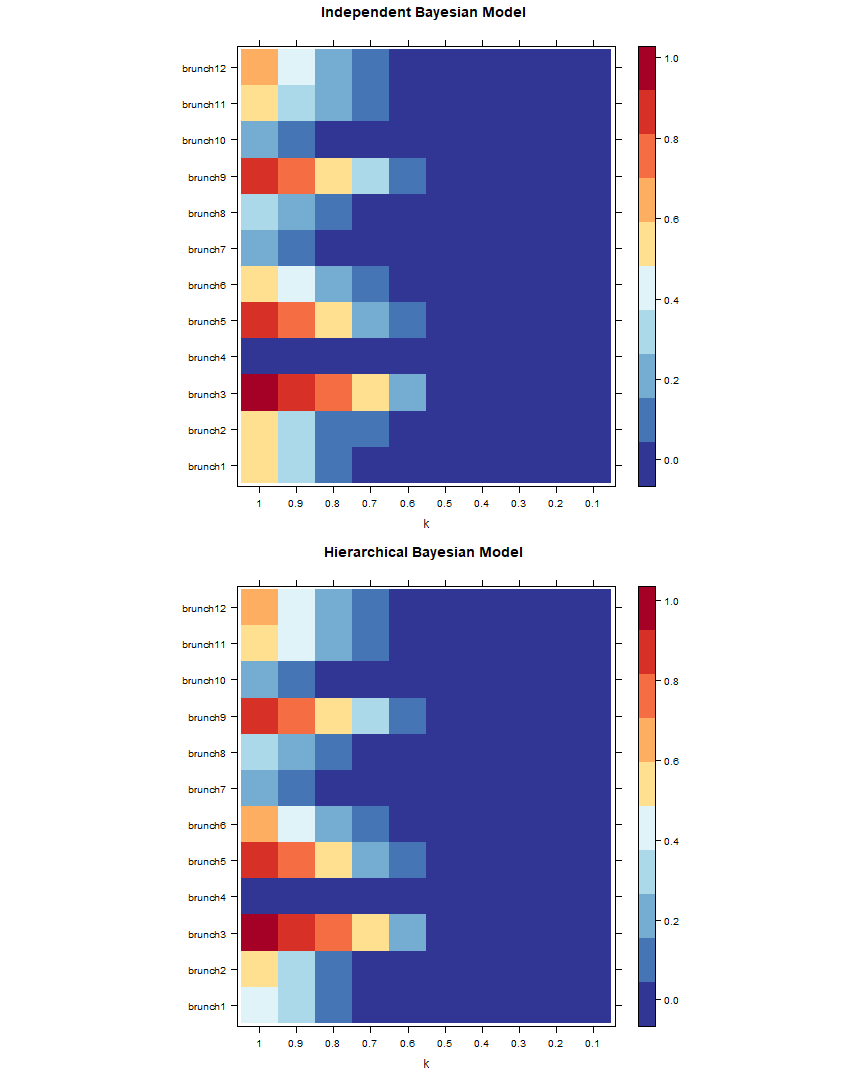
\includegraphics[width=1\linewidth]{../../R-codes/JAGS/plots/sim2/heattotal}
			\caption{Heat-map of anomaly signals for different different hierarchical structure, of IBM and HBM at category total.}
			\label{fig:heattotal3}
		\end{figure}
		
		\newpage
		
		\begin{figure}[!h]
			\centering
			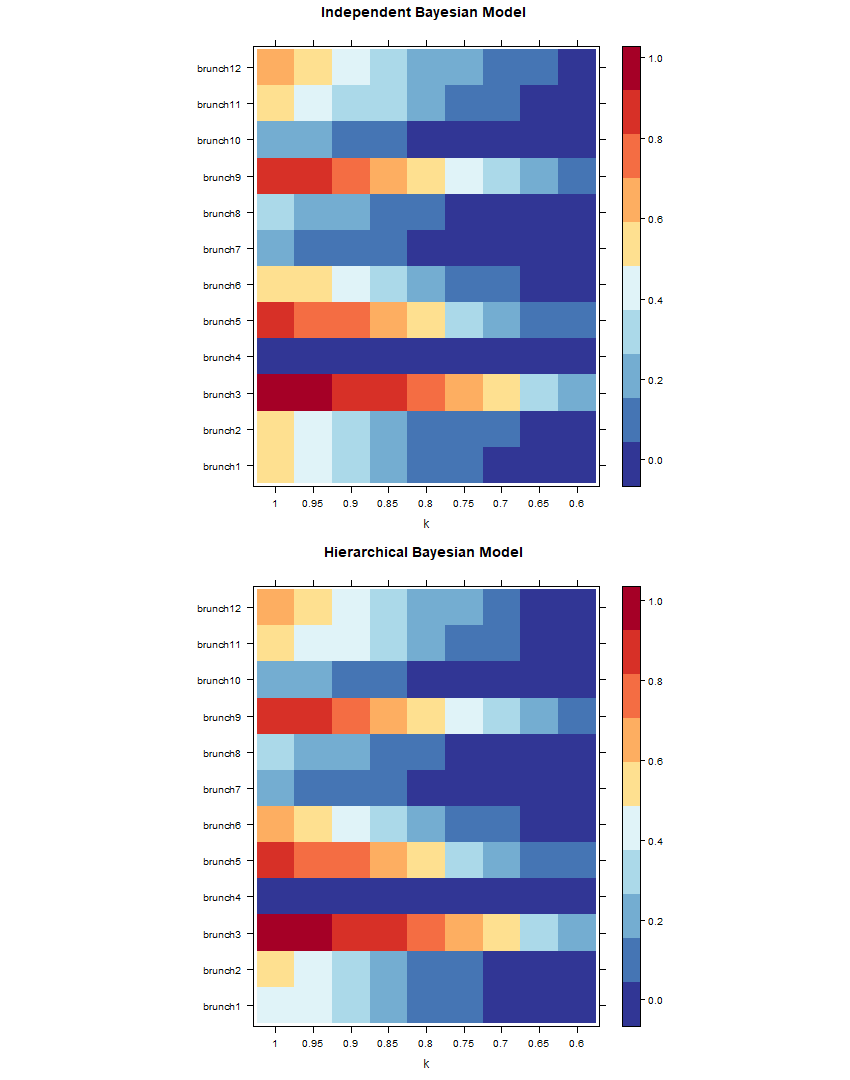
\includegraphics[width=1\linewidth]{../../R-codes/JAGS/plots/sim2/heattotal2}
			\caption{Heat-map of anomaly signals for different different hierarchical structure, of IBM and HBM zoomed in at k values of 0.6 to 1, at category total.}
			\label{fig:heattotal3h}
		\end{figure}
		
		\newpage
		
		The heat-map in figure~\ref{fig:heattotal3} presents the anomaly signals of category total for different hierarchical structures with the addition of a constant anomaly, with IBM and HBM, against different increments of $k$. There is no apparent trend in anomaly signals terms of the number of branch at category AA, of category total. However,  it is relatively clear that stronger signals of anomaly seem to locate at left sider of the heat-map, indicating that higher the $k$, stronger the signal. Zooming in at looking at k values from 0.6 to 1 in figure~\ref{fig:heattotal3h}, we observe a noticeable small difference in anomaly detection rate between IBM and HBM for category total. Our observation suggests that the difference between anomaly detection rate is small or close to none for IBM and HBM, on the top level of the hierarchy, for anomaly with a different hierarchical structure, in a simulated setting with each category generated independently. 
		
		\newpage
		
		\begin{figure}[!h]
			\centering
			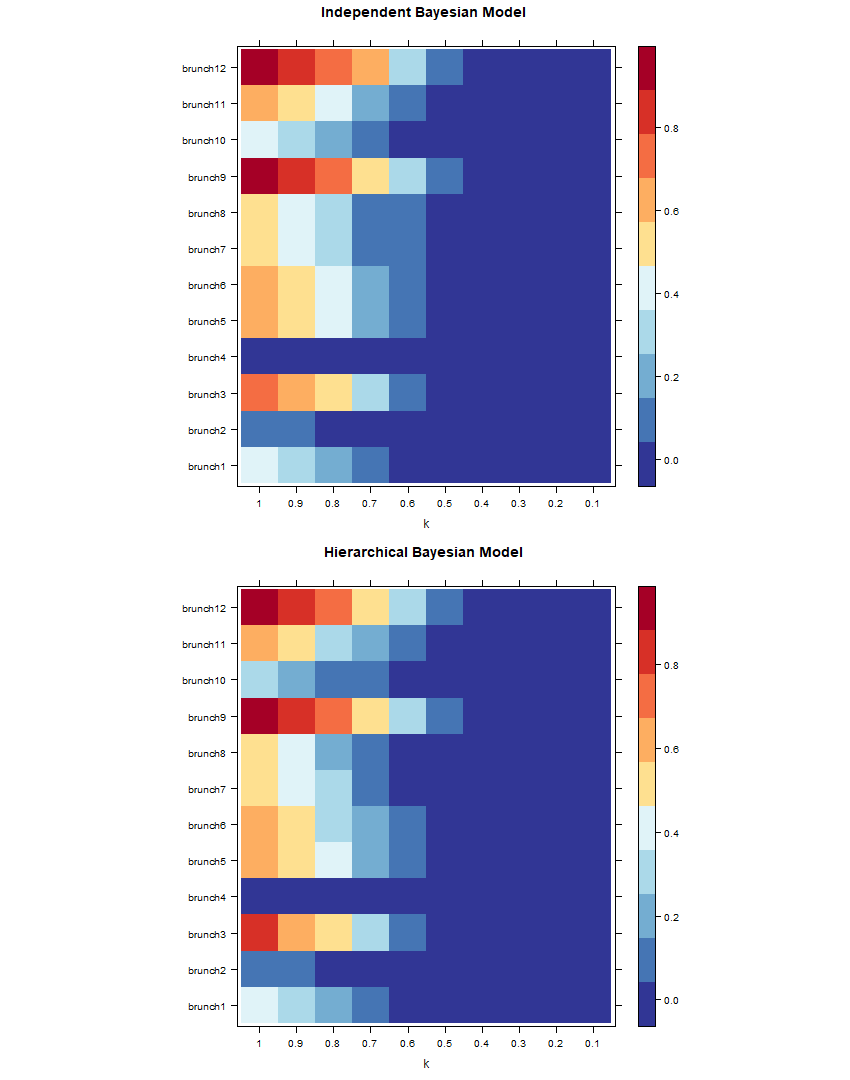
\includegraphics[width=1\linewidth]{../../R-codes/JAGS/plots/sim2/heatA}
			\caption{Heat-map of anomaly signals for different different hierarchical structure, of IBM and HBM, at category A.}
			\label{fig:heatA3}
		\end{figure}
		
		\newpage
		
		\begin{figure}[!h]
			\centering
			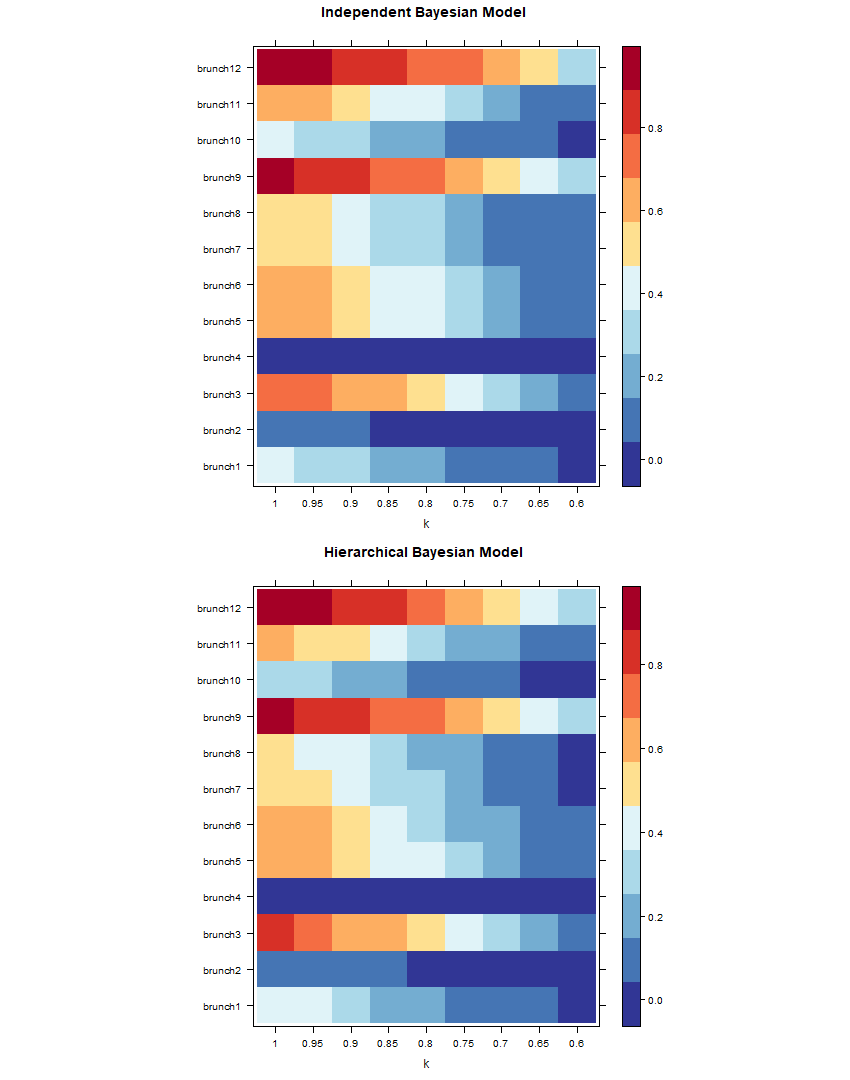
\includegraphics[width=1\linewidth]{../../R-codes/JAGS/plots/sim2/heatA2}
			\caption{Heat-map of anomaly signals for different different hierarchical structure, of IBM and HBM zoomed in at k values of 0.6 to 1, at category A.}
			\label{fig:heatA3h}
		\end{figure}
		
		\newpage
		
		The heat-map in figure~\ref{fig:heatA3} presents the anomaly signals of category A for different hierarchical structures with the addition of a constant anomaly, with IBM and HBM, against different increments of $k$. There is no apparent trend in anomaly signals terms of the number of branch at category AA, of category A. However,  it is relatively clear that stronger signals of anomaly seem to locate at left sider of the heat-map, indicating that higher the $k$, stronger the signal. Zooming in at looking at k values from 0.6 to 1 in figure~\ref{fig:heatA3h}, we observe a noticeable small difference in anomaly detection rate between IBM and HBM for category A. Our observation suggests that the difference between anomaly detection rate is small or close to none for IBM and HBM, on level 2 of the hierarchy, for anomaly with a different hierarchical structure, in a simulated setting with each category generated independently. 
		
		\newpage
		
		\begin{figure}[!h]
			\centering
			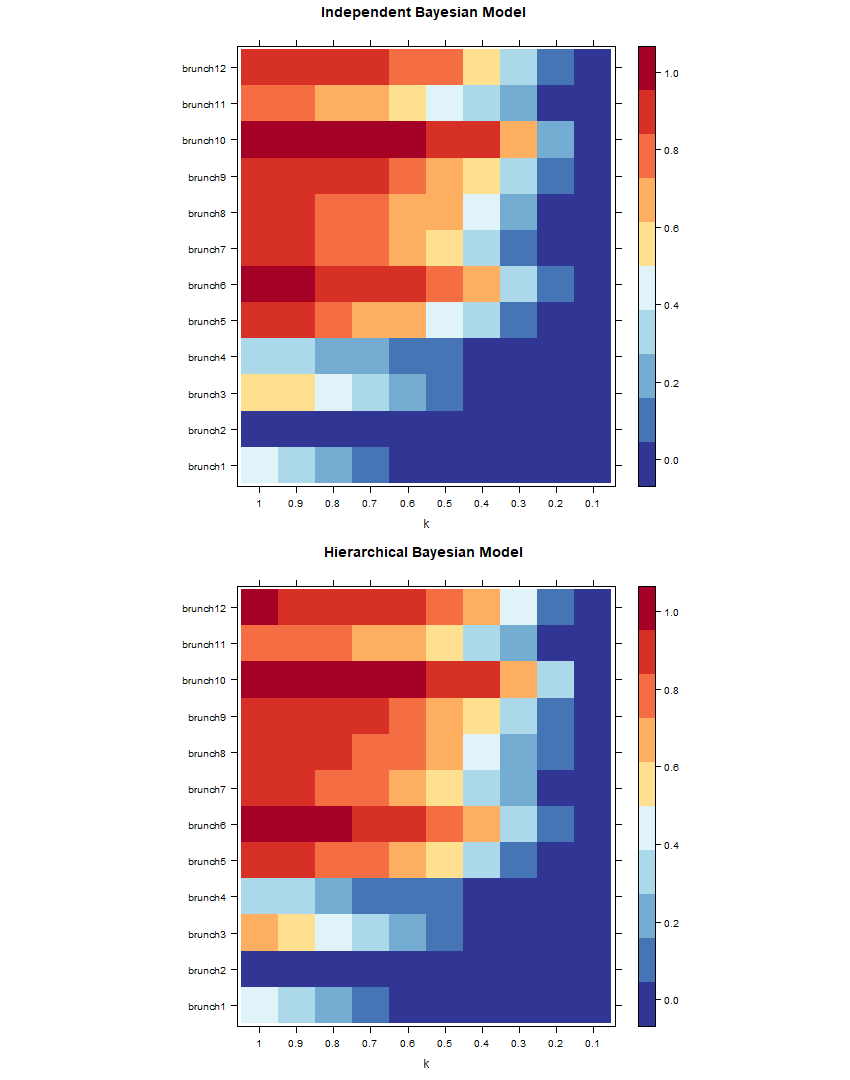
\includegraphics[width=1\linewidth]{../../R-codes/JAGS/plots/sim2/heatAA}
			\caption{Heat-map of anomaly signals for different different hierarchical structure, of IBM and HBM, at category AA.}
			\label{fig:heatAA3}
		\end{figure}
		
		\newpage
		
		\begin{figure}[!h]
			\centering
			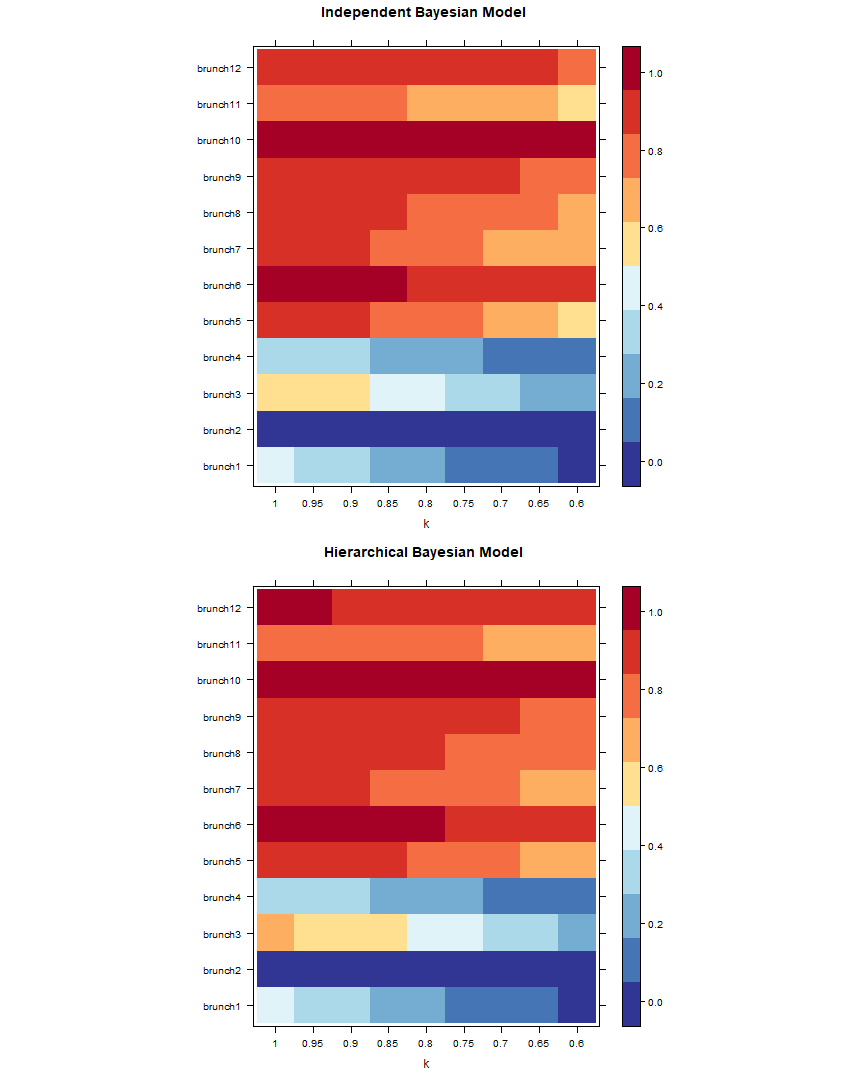
\includegraphics[width=1\linewidth]{../../R-codes/JAGS/plots/sim2/heatAA2}
			\caption{Heat-map of anomaly signals for different different hierarchical structure, of IBM and HBM zoomed in at k values of 0.6 to 1, at category AA.}
			\label{fig:heatAAh3}
		\end{figure}
	
	\newpage
		
		The heat-map in figure~\ref{fig:heatAA3} presents the anomaly signals of category A for different hierarchical structures with the addition of a constant anomaly, with IBM and HBM, against different increments of $k$. Unlike previous categories, anomaly signals tend to get stronger as the number of branching increases. It is also very clear that stronger signals of anomaly seem to locate at left side of the heat-map, indicating that higher the $k$, stronger the signal. Zooming in at looking at k values from 0.6 to 1 in figure~\ref{fig:heatAAh3}, we observe a noticeable small difference in anomaly detection rate between IBM and HBM for category AA. Our observation suggests that the difference between anomaly detection rate is small or close to none for IBM and HBM, on the bottom of the hierarchy, for anomaly with a different hierarchical structure, in a simulated setting with each category generated independently. 
		
		\newpara
		
		Overall we see that there are slight differences in signals fro IBM and HBM results, and if we zoom in and look at a smaller interval of $k$, the difference are more apparent. HBM tend to give strong signals than IBM. Because we simulated datasets used for each scenario independently, there is a lot of uncertainty and noise and made it hard to distinguish differences and trends. However, at the bottom level, where the difference in structure takes place, the effect of noise does not seem to mask the trends any more. Comparing across levels, we see that the top hierarchy have the lowest signal overall, and the bottom hierarchy have the strongest signal overall. 
		
		\subsection{Discussion}
		
		Our DIC results yield similar results as what we have in the previous simulation, that HBM gives better goodness of fit and is the better model, for scenarios with different hierarchical structures. Our finding could suggest that HBM gives better goodness of fit consistently, for hierarchies with different hierarchical structures. These findings add to the reliability of HBM and suggesting it to be a versatile model that is superior to IBM in different settings and for different hierarchical structures. Because we had synthesised datasets used for our scenarios independently, we have a higher level of uncertainty compare to our previous simulation. It adds to the uncertainty we already had from Bayesian estimations and made it even harder to explore for differences and trends. A possible remedy is to use the same dataset, but for branching that take place in category AA, we could try to generate values for its children categories randomly, with statistical techniques such as bootstrapping. 
		
		\newpara
		
		An interesting observation is that trends and differences in category AA seem to have overcome the making effect by the noise and are a lot more clear than what we observe in higher categories. It is partly due to the fact that HBM tend to retain more information ( there is more information at a lower level of hierarchy) at lower levels of hierarchy and the amount of information is significant enough for HBM to produce results that have a stronger presence than randomness. Another possibility is that it has something to do with influences of extra information that we created for Category A and it's children during our data synthesis process, which is retained by HBM but not at all present in IBM. 
		
		
		

	\chapter{MIMIC-III}\label{chap:MIMIC}

\section{Introduction}

We carried-out simulations with synthetic patient arrival datasets, and compares the posterior distribution results and prediction rate between Independent Bayes Model (IBM) and Hierarchical Bayes Model (HBM) for-real life data, for the scenarios of common, rare and extremely rare diseases. Sections 3.2 to 3.8 provides background information about the MIMIC-III database. Sections 3.9 gives the result of our analyses. Lastly,  Section 3.10 forms our discussion. 

\section{Source of Data}

For this thesis, datasets from the Medical Information Mart for Intensive Care version 1.4 (MIMIC-III v1.4) database, available on PhysioNet Clinical Databases (\href{https://mimic.physionet.org}{https://mimic.physionet.org}), was used. MIMIC-III is a large, open-access, well maintained database with a collection of de-identified health-related data associated with over 58,000 hospital admissions for 38,645 adults and 7,875 neonates, who was admitted to critical care units of the Beth Israel Deaconess Medical Center (Boston, MA, USA) between the period of June 2001 and October 2012 and is hosted by the Laboratory for Computational Physiology (LCP) at the Massachusetts Institute of Technology (MIT) \citep{johnson2016mimic,Pollard2016mimic,goldberger2000physiobank}. MIMIC-III contains clinical, physiological, and mortality data aggregated from ICU information systems, digital hospital archives, bedside monitors and Social Security Administration Death Master Files. MIMIC-III includes health-related information such as demographics, vital sign measurements, laboratory test results, procedures, medications, caregiver notes, imaging reports, and in and out of hospital mortality registry. Data were collected continuously with non-invasive procedures during routine clinical care and data collection and was blinded from patient and staff, minimising interference with medical routine. Private health information was also de-identified to protect patient privacy \citep{Mark2016}. For example, all dates in the database have been shifted to periods between 2100 to 2200 while conserving seasonal trends. 

\newpara

Access and use of the MIMIC-III database for this thesis have been authorised with a restricted-access to PhysioNet clinical databases and bound by a data use agreement, approved on 9th April 2019. 

\section{ICD-9}

According to the World Health Organisation \citep{WHO2019}, International Statistical Classification of Diseases and Related Health Problems (ICD) is the international standard for clinical diagnosis. ICD defines diseases, disorders, injuries, and other related health conditions in a hierarchical fashion, this allows for storage and access of health-related information internationally, in other words, ICD is the standard for clinical diagnosis. Though there is a subtle variation to the standard as some country adopt different versions. For example, Clinical Modification (ICD-9-CM) is an adaption used in assigning diagnostic in the United States \citep{CDC2019}, and in New Zealand, the Australian Modification (ICD-10-AM) were used \citep{MoH2019}. The version of ICD used for medical diagnosis in the MIMIC dataset is ICD-9, the codes are assigned at the end of the patient’s stay and are used by the hospital to bill for care provided \citep{johnson2016mimic}.

\newpara

\begin{figure}[h]
	\centering
	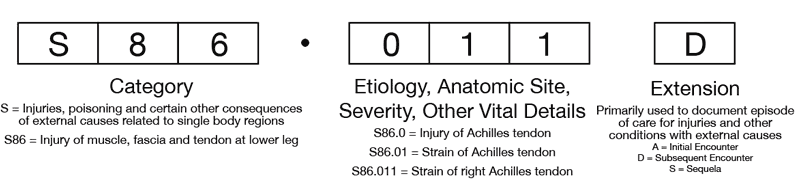
\includegraphics[width=0.7\linewidth]{Figures/icd-10-code}
	\caption{Visualisation of ICD-10 Code Structure, from \cite{Andrus2013}.}
	\label{fig:icd10code}
\end{figure}

As shown in figure~\ref{fig:icd10code}, the first three characters of an ICD codes designate the category of the diagnosis, followed by supplementary information of aetiology (i.e., the cause of condition), anatomic site, severity, or other vital clinical details after a full stop, and may contain an extension used to document episodes of care, this was implemented for ICD 10. For some instances, there may be multiple codes entries for a single condition, like in the case of an Achilles tendon strain, secondary external cause code may be provided along with the primary diagnosis. 

\newpage 

\begin{table}[h!]
	\centering
	\begin{tabular}{|rll|} 
		\hline
		\textbf{Series} & \textbf{ICD-9 Label}  & \textbf{Description}\\ [0.5ex] 
		
		\hline\hline
		\textit{Total}&&\\
		
		1 & -  & International Classification of Diseases, 9th Revision \\ 
		
		\hline    
		\textit{Category lv1}&&\\
		
		1 &001-139  &Infectious And Parasitic Diseases\\
		2 &140-239  &Neoplasms\\
		3 &240-279  &Endocrine, Nutritional And Metabolic Diseases, And \\
		&& Immunity Disorders\\
		...&...&...\\
		17 &800-999  &Injury And Poisoning\\
		18 &V01-V91  &Supplementary Classification Of Factors Influencing \\
		&&Health Status And Contact With Health Services\\
		19 &E000-E999  &Supplementary Classification Of External Causes Of\\
		&& Injury And Poisoning\\
		
		\hline    
		\textit{Category lv2}&\textit{(001-999)}&\\
		
		1 &001-009  &Intestinal Infectious Diseases\\
		2 &010-018  &Tuberculosis\\
		3 &020-027  &Zoonotic Bacterial Diseases\\
		...&...&...\\
		35 &980-989  &Toxic Effects Of Substances Chiefly Nonmedicinal As\\ 
		&&To Source\\
		36 &990-995  &Other And Unspecified Effects Of External Causes\\
		37 &996-999  &Complications Of Surgical And Medical Care, Not \\
		&&Elsewhere Classified\\
		
		\hline    
		\textit{Category lv3}&\textit{(001-999)}&\\
		
		1 &001 &Cholera\\
		2 &002 &Typhoid and paratyphoid fevers\\
		3 &003 &Other salmonella infections\\
		\...&...&...\\
		89&997 &Complications affecting specified body system not \\
		&& elsewhere classified\\
		89&998 &Other complications of procedures not elsewhere \\
		&&classified\\
		89&999 &Complications of medical care not elsewhere classified\\
		
		\hline
		
	\end{tabular}
	\caption{ICD-9 Diagnosis Codes}
	\label{fig:icd10table}
\end{table}

\newpage

ICD 9 categories are coded from 001 to 999, with two extra supplementary class of categories starting with V and E. For example, 001 code for Cholera, and E880 is the code for Accidental fall on or from stairs or steps. Several categories are aggregated to form a larger category, and there are two aggregations which made ICD a three-level hierarchical structure. Following Cholera at level 3, it is aggregated into Intestinal Infectious Diseases for categories from 001 to 009 at level 2, and Infectious and Parasitic Diseases for the categories from 001 to 139 at level 1. Level 1 categories are sometimes referred to as chapters. ICD groupings help to provide a picture of the health situation of the general populations. This information is useful in health care management, and allocation of resources, and other health-related decision-making processes, such as billing of services. Table~\ref{fig:icd10table} provides some examples of ICD codes in different level of ICD categories. There are 632 categories at level 3 of the hierarchy, as those descibed in Table~\ref{fig:icd10table}, there are even finer categories, and national adaptions. ICD-10-CM (usedin USA), for example, has over 70,000 distinct codes \cite{ICD2019}. 

\section{Study Population }

Study inclusion criteria were ICU admission of patients of all age with available documentation of primary ICD-9 diagnosis, excluding supplementary diagnoses (ICD codes start with V or E). Repeated admission to ICU by the same patient were included. The final dataset used contain 50959 uniquely identified Hospital admission event with 38869 uniquely identified patients. 

\section{Study Variables}

Three datasets were merged, including the admissions table, the diagnoses\_icd table and the d\_icd\_diagnoses table. Hospital Admission ID and Subject Id were used to as key identifiers. No demographic information was collected, some event-related information were included, these include Admission time, admission type and admission location. Admission time was converted to admission date. ICD-9 codes used only to contain the first three digits of the full ICD code, the reason for it is that further digits do not reflect any categorical characteristics and will only increase the number of non-significant sub-categories. Supplementary ICD codes that start with V or E were not used, which meant we have ICD codes range from 001 to 999. We defined level 2 and level 3 ICD categories according to the standard ICD-9 definition and created flag/dummy variables for each category. There are 132 unique level 2 ICD categories and 631 unique level 3 ICD categories that were created. Short and long title associated with ICD codes were also included. 

\section{Model}

This section presents the Independent Bayesian Model(IBM) and Hierarchical Bayesian Model(HBM) that is used to calculate posterior distributions. 

\newpara

It is believed that time series prediction are a good prior belief that makes sense, we do not know what the arrival for today will be but we can make an educated guess using our historical records. predictions about the expected daily arrival are used as our prior values, with data for all observed values for the dates prior to the prediction date, using \texttt{predict.hts} Function inside the R environment. Forecast method used is Autoregressive integrated moving average (ARIMA), prediction function used is \texttt{tbats}, and parallel processing is activated to speed up the prediction process. Examples of R-codes used for the time series prediction can be found in Appendix~\ref{htsp}. 

\newpara

For the IBM model, predictions are made with the bottom-up approach by setting argument \texttt{method = "bu"}, the reason for it is that the bottom-up approach makes independent predictions at the leaf level, and does not take into account the hierarchical structure of the data and are suitable for IBM model. In the other hand, predictions for the IBM model are made with the optimal reconciliation approach by setting argument \texttt{method = "comb"}, optimal reconciliation approach reconciles prediction from individual time forecasts from all levels and gives an optimum solutions as the forecast, which meant that the approach takes into account the hierarchical structure of the data, and are suitable for HBM model. However, current optimum solutions will give nonsensical negative predictions. However, these negative solutions are mostly extremely small and close to 0 and are therefore simply converted to 0. So the optimal reconciliation forecasts used for our HBM model are not the actual optimum solution, but the adjusted optimal solution. Non-negativity optimal reconciliation for the \texttt{predict.hts} the function is currently being developed and will be released on CRAN in late July, after the submission date of this thesis. 

\newpara

A Normal(1,0.1) distribution is multiplied with the predicted values to add distribution properties to our prior as our weakly-informative prior. For IBM posterior distributions, posteriors of each category are independently calculated with an IBM model. Whereas for HBM posterior distributions, posterior for each category is calculated with an HBM model that considers all of the levels within the hierarchy. JAGS-codes used to build the IBM and HBM are provided in Appendix~\ref{ibmhbm} and Appendix~\ref{ibmhbm2}. 

\newpara

The likelihood model used for our IBM is:

\begin{equation} \label{ibma8}
\begin{aligned}
y_{i,t} & \sim Poisson(\mu_{i,t}) \\  
log(\mu_{i,t}) & = log(\rho_{i,t}\lambda_{i,t}) \\
\end{aligned}
\end{equation}

Priors for model parameters for our IBM is:

\begin{equation} \label{ibm8b}
\begin{aligned}
\lambda_{i,t} & \sim Normal(\mu_{i,t},\sigma_{i,t}) T_{[\lambda>0]}\\
\end{aligned}
\end{equation}

Hyper-priors for model parameters for our IBM is:

\begin{equation} \label{ibmc8}
\begin{aligned}
\mu_{i,t} & \sim Normal(1,0.1)\\
\sigma^2_{i,t} &\sim Normal(0.1,0.1)\\
\end{aligned}
\end{equation}

The likelihood model used for our HBM is also:

\begin{equation} \label{hbma8}
\begin{aligned}
y_{i,t} & \sim Poisson(\mu_{i,t}) \\  
log(\mu_{i,t}) & = log(\rho_{i,t}\lambda_{i,t}) \\
\end{aligned}
\end{equation}

But $\lambda_{i,t}$ used for different levels of the hierarchy are interconnected with priors and hyper-priors and hyper-hyper priors and so on, that captures the hierarchical structure of our ICD-9 categories.

\newpara

For level 0 category(total):

\begin{equation} \label{hbm8b}
\begin{aligned}
\lambda_{(lv0)i,t} & \sim Normal(\mu_{(lv0)i,t},\sigma_{(lv0)i,t}) T_{[\lambda>0]}\\
\mu_{(lv0)i,t} & \sim Normal(1,0.1)\\
\sigma^2_{(lv0)i,t} &\sim Normal(0.1,0.1)\\
\end{aligned}
\end{equation}

For level 1 categories:

\begin{equation} \label{hbm8b}
\begin{aligned}
\lambda_{(lv1)i,t} & \sim Normal(\mu_{(lv1)i,t},\sigma_{(lv1)i,t}) T_{[\lambda>0]}\\
\mu_{(lv1)i,t} & \sim Normal(mu_{(lv0)i,t},0.1)\\
\sigma^2_{(lv1)i,t} &\sim Normal(0.1,0.1)\\
\end{aligned}
\end{equation}

For level 2 categories:

\begin{equation} \label{hbm8b}
\begin{aligned}
\lambda_{(lv2)i,t} & \sim Normal(\mu_{(lv2)i,t},\sigma_{(lv2)i,t}) T_{[\lambda>0]}\\
\mu_{(lv2)i,t} & \sim Normal(\mu_{(lv1)i,t},0.1)\\
\sigma^2_{(lv2)i,t} &\sim Normal(0.1,0.1)\\
\end{aligned}
\end{equation}

For level 3 (leaf-level) categories:

\begin{equation} \label{hbm8b}
\begin{aligned}
\lambda_{(lv3)i,t} & \sim Normal(\mu_{(lv3)i,t},\sigma_{(lv3)i,t}) T_{[\lambda>0]}\\
\mu_{(lv3)i,t} & \sim Normal(\mu_{(lv2)i,t},0.1)\\
\sigma^2_{(lv3)i,t} &\sim Normal(0.1,0.1)\\
\end{aligned}
\end{equation}


\section{Anomaly} 

The date of 10 November 2190 is set up to be the default date for anomalies additions, therefore, for yearly data anomaly is added on the year of 2190, for monthly data the anomaly is added on 2090Nov, and so on. Due to limitations in sample size and complexity of the ICD-9 hierarchy, it is decided that the time period that we would use is yearly periods between years of 2100 to 2290, the mimic-3 dataset provides an average of 500 arrivals per year.

\newpara

We are interested in how the anomaly detection rates of Independent Bayesian Model (IBM) and Hierarchical Bayesian Model(HBM) will perform for arrivals of common, rare and extremely rare disease diagnoses. \textbf{Common} disease refers to a disease that public hospitals will likely to always encounter in a time period, in our case we decided to choose category 410, which codes for Acute myocardial infarction, commonly known as a heart attack. There are 3307 cases of Acute myocardial infarction in the MIMIC-III data, making it one of the largest category. Considering the pre-perturbation time period used in MIMIC-III is actually a 12 year period. We can suggest that Acute myocardial infarction as a common disease that the ICU department almost sees daily. \textbf{Rare} disease refers to a disease that public hospitals will unlikely to encounter in a time period, in our case we decided to choose category 415, which codes for Acute pulmonary heart disease, also known as cor pulmonale, is the enlargement and failure of the right ventricle of the heart as a response to increased vascular resistance (such as from pulmonic stenosis) or high blood pressure in the lungs.\citep{MedlinePlus2019}. There are 373 cases of Acute pulmonary heart disease in the MIMIC-III data,  considering the pre-perturbation time period of MIMIC-III is actually a 12 year period, we can suggest that Acute myocardial infarction as a rare disease that the ICU department almost sees monthly. \textbf{Extremely rare} disease refers to a disease that public hospitals will extremely unlikely to encounter in a time period, in our case we decided to choose category 452, which codes for Portal vein thrombosis, it is blockage or narrowing of the portal vein by a blood clot \citep{MSD2019}. There are only 12 cases of Acute pulmonary heart disease in the MIMIC-III data,  considering the pre-perturbation time period of MIMIC-III is actually a 12 year period, we can suggest that Acute myocardial infarction as an extremely rare disease that the ICU department are lucky to see more than once per year. 

\newpara

Three abnormal yearly observations are created to test anomaly detection of the three scenarios when there is definitely anomaly (we added anomaly) present at the lowest level of the hierarchy. Due to the aggregation constraint, the addition of anomaly at the lowest level of the hierarchy will result in the addition of the same number of anomalies to its parent and ancestors. This has an effect on the detection rate in all levels of the hierarchy that relates to the specific category. If the observation is 0, a default anomaly of 1 is added. 

\newpara

%\begin{figure}
%    
%    \caption{Addition of 100\% anomaly to common, rare and extremely rare diseases. }
%    \label{fig:addano}
%\end{figure} 

Overall we are looking at four scenarios. Scenario 1 is the anomaly detection rate of common, rare and extremely rare disease categories of the observed data, without the addition of an anomaly. Scenario 2 is the anomaly detection rate of common disease categories of the observed data, with an addition 100\% anomaly at the lowest hierarchy level. Scenario 3 is the anomaly detection rate of rare disease categories of the observed data, with an addition 100\% anomaly at the lowest hierarchy level. Lastly, in scenario 4, we look at the anomaly detection rate of extremely rare disease categories of the observed data, with an addition 100\% anomaly at the lowest hierarchy level. 

\section{Statistical Analyses}

A DIC comparisons table was first used to compare the difference in DIC distributions of Independent Bayesian Model (IBM) and Hierarchical Bayesian Model (HBM). Posterior distributions of our categories of interest for original and anomaly data are then provided in tables and density plots. Lastly, signals of the anomaly are visualised with a heat-map. SAS version 9.4 \citep{SAS} was used during the data cleaning process, and analyses were performed with R version 3.3.2 \citep{R} in the R Studio environment Version 1.1.463 \citep{Rstudio}. An overview of functions created and models built in this thesis is provided in the Appendix. The full collection of R, JAGS, and SAS codes used to synthesise datasets, clean and merge datasets, run the simulation, and draw table and plots and are available on GitHub repository
\href{https://github.com/jungxue/research-masters-Jung}{https://github.com/jungxue/research-masters-Jung}.

%=============================== Results =====================================

\newpage

\section{Results}

%----------------------------- DIC ----------------------------------

\begin{table}[!h]
	\centering
	\begin{tabular}{rrrrrrrr}
		\hline
		& Min. & 1st Qu. & Median & Mean & 3rd Qu. & Max. & NA's \\ 
		\hline
		No amomaly & -5.635 & -0.443 & -0.004 & 0.095 & 0.494 & 9.212 & 109 \\ 
		410 & -5.579 & -0.416 & 0.005 & 0.118 & 0.547 & 6.933 & 109 \\ 
		415 & -7.660 & -0.438 & -0.010 & -0.007 & 0.444 & 8.195 & 109 \\ 
		452 & -6.540 & -0.466 & -0.002 & 0.048 & 0.496 & 7.628 & 109 \\ 
		\hline
	\end{tabular}
	\caption{DIC comparisons for Independent Bayesian Model and Hierarchical Bayesian model for no anomaly, and anomaly added for common, rare and extremely rare diseases} 
	\label{tab:dicmimic}
\end{table}

\newpara

Table~\ref{tab:dicmimic} gives the comparison of DIC distributions of Independent Bayesian Model (IBM) and Hierarchical Bayesian Model (HBM) for no anomaly, and anomaly added for common, rare and extremely rare diseases. It is tough to tell whether or not HBM perform better than IBM, because the negative signal is very hard to detect, and the mean and median value is very close to 0. Multiple samples of DIC are also not feasible as sampling process took a very long time. Conclusions about goodness-of-fit performance between IBM and HBM can not be made. 



%----------------------------- Posteriors ----------------------------------

\newpage

\begin{table}[!t]
	\centering
	\begin{tabular}{rrrrrrrr}
		\hline
		& mean & sd & 2.5\% & 50\% & 97.5\% & Rhat & n.eff \\ 
		\hline
		total & 526.647 & 22.818 & 482.137 & 526.444 & 573.014 & 1.000 & 2912.000 \\ 
		390-459 & 195.270 & 13.662 & 169.633 & 194.978 & 222.341 & 1.000 & 3000.000 \\ 
		410-414 & 78.372 & 8.798 & 62.315 & 78.048 & 95.974 & 1.000 & 2888.000 \\ 
		415-417 & 3.240 & 1.815 & 0.715 & 2.917 & 7.654 & 1.000 & 2415.000 \\ 
		451-459 & 6.412 & 2.555 & 2.477 & 6.048 & 12.171 & 1.000 & 2191.000 \\ 
		410 & 37.218 & 6.211 & 26.305 & 36.663 & 50.562 & 1.000 & 2879.000 \\ 
		415 & 3.293 & 1.833 & 0.800 & 2.932 & 7.714 & 1.000 & 1977.000 \\ 
		452 & 0.158 & 0.174 & 0.001 & 0.087 & 0.597 & 1.010 & 445.000 \\ 
		\hline
	\end{tabular}
	\caption{Posterior distributions for ICD 410,415 and 452 and its ancestors, with no added anomalies, and calculated with Independent Bayes Model} 
	\label{tab:postsumnorm.mimic}
\end{table}

\begin{figure}[!h]
	\centering
	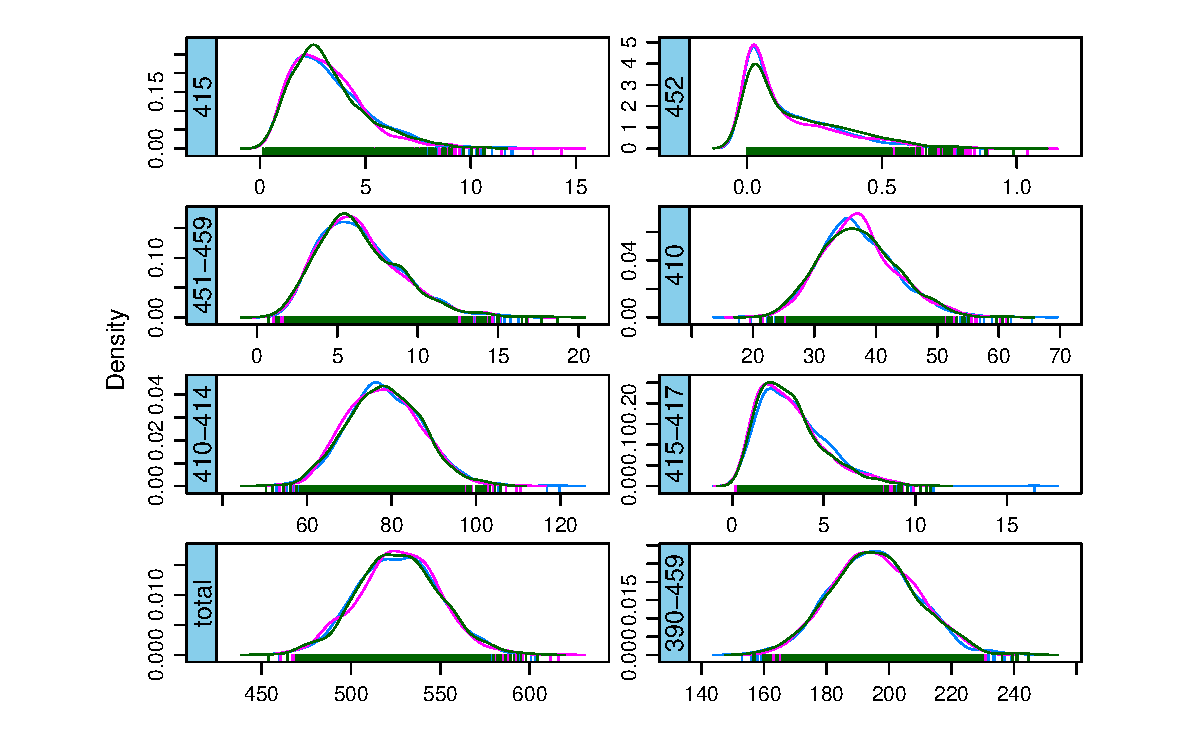
\includegraphics[width=1\linewidth]{../../R-codes/JAGS/plots/mimic/Densitynorm}
	\caption{Posterior distributions for ICD 410,415 and 452 and its ancestors, with no added anomalies, and calculated with Independent Bayes Model}
	\label{fig:densitynorm}
\end{figure}

\newpage

\begin{table}[!t]
	\centering
	\begin{tabular}{rrrrrrrr}
		\hline
		& mean & sd & 2.5\% & 50\% & 97.5\% & Rhat & n.eff \\ 
		\hline
		total & 525.996 & 22.917 & 482.084 & 525.396 & 572.556 & 1.000 & 3000.000 \\ 
		390-459 & 194.540 & 14.077 & 167.744 & 194.275 & 223.211 & 1.000 & 3276.000 \\ 
		410-414 & 78.348 & 8.939 & 62.045 & 77.995 & 96.766 & 1.000 & 3160.000 \\ 
		415-417 & 3.116 & 1.734 & 0.692 & 2.817 & 7.201 & 1.000 & 2174.000 \\ 
		451-459 & 6.288 & 2.344 & 2.516 & 6.053 & 11.522 & 1.010 & 1401.000 \\ 
		410 & 37.678 & 6.166 & 26.738 & 37.342 & 50.959 & 1.000 & 3000.000 \\ 
		415 & 3.319 & 1.949 & 0.703 & 2.954 & 8.441 & 1.000 & 1990.000 \\ 
		452 & 0.150 & 0.169 & 0.001 & 0.082 & 0.607 & 1.050 & 279.000 \\ 
		\hline
	\end{tabular}
	\caption{Posterior distributions for ICD 410,415 and 452 and its ancestors, with no added anomalies, and calculated with Hierarchical Bayes model} 
	\label{tab:postsumnormh.mimic}
\end{table}

\begin{figure}[!h]
	\centering
	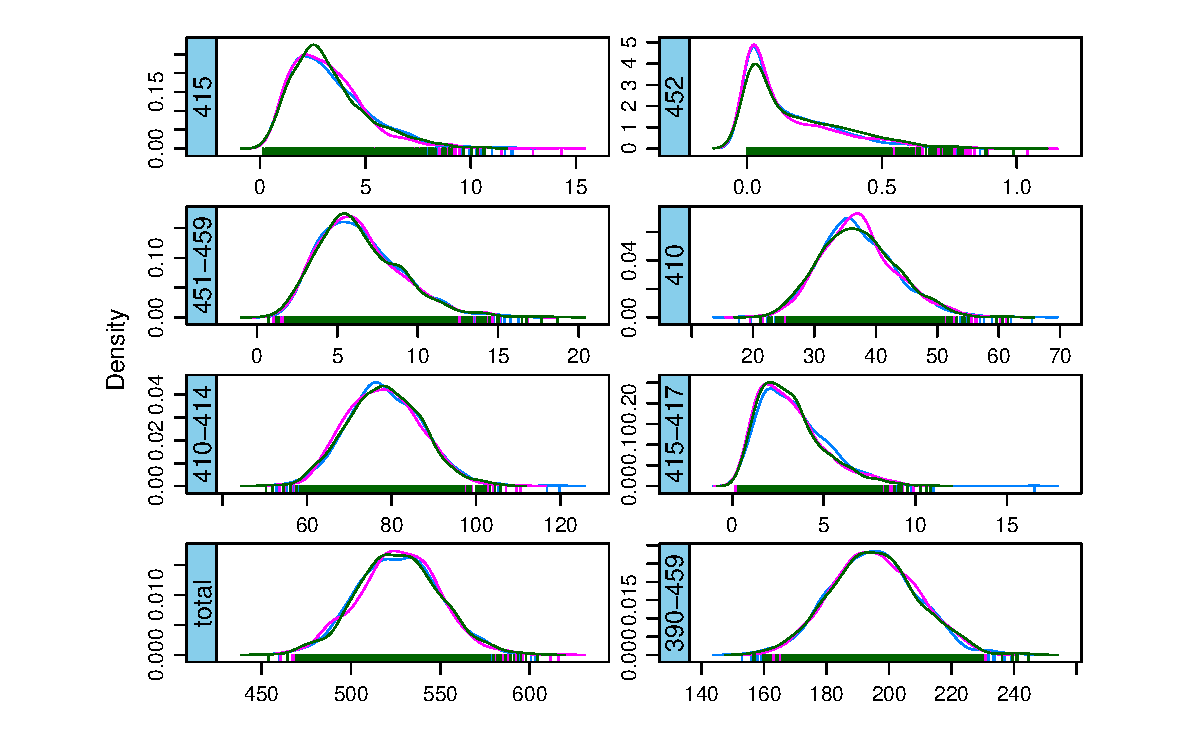
\includegraphics[width=1\linewidth]{../../R-codes/JAGS/plots/mimic/Densitynorm}
	\caption{Posterior distributions for ICD 410,415 and 452 and its ancestors, with no added anomalies, and calculated with Hierarchical Bayes model}
	\label{fig:densitynormh}
\end{figure}

Table~\ref{tab:postsumnorm.mimic} and figure~\ref{fig:densitynorm} shows the posterior for IBM and table~\ref{tab:postsumnormh.mimic} and figure~\ref{fig:densitynormh} shows the posterior for HBM, for ICD 410,415 and 452 and its ancestors, with no added anomalies. There are no obvious differences between the distribution values and distribution shape for IBM and HBM. Distribution for categories at a higher level, and categories with higher mean values tend to approximate to normal, for the case of category 415-417, even though it is at a higher hierarchy level it has a low mean, and the distribution is not normal. 

\newpage%----------------------------------- 410 -------------------------------------------

\begin{table}[!t]
	\centering
	\begin{tabular}{rrrrrrrr}
		\hline
		& mean & sd & 2.5\% & 50\% & 97.5\% & Rhat & n.eff \\ 
		\hline
		total & 563.697 & 23.816 & 518.412 & 563.222 & 612.356 & 1.000 & 3111.000 \\ 
		390-459 & 232.494 & 15.041 & 204.686 & 231.814 & 263.502 & 1.000 & 2905.000 \\ 
		410-414 & 115.402 & 10.918 & 94.819 & 114.956 & 137.937 & 1.000 & 3000.000 \\ 
		410 & 74.630 & 8.617 & 58.748 & 74.137 & 92.840 & 1.000 & 3542.000 \\ 
		\hline
	\end{tabular}
	\caption{Posterior distributions for ICD 410 and its ancestors, with added anomalies, and calculated with independent Bayes model} 
	\label{tab:postsum410.mimic}
\end{table}

\begin{figure}[!h]
	\centering
	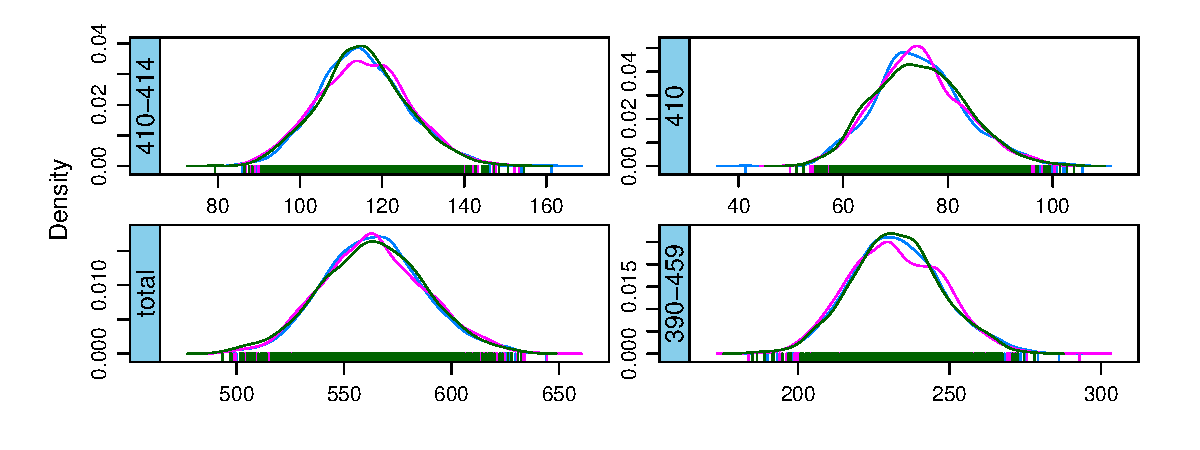
\includegraphics[width=1\linewidth]{../../R-codes/JAGS/plots/mimic/Density410}
	\caption{Posterior distributions for ICD 410 and its ancestors, with added anomalies, and calculated with independent Bayes model}
	\label{fig:density410}
\end{figure}

\newpage%----------------------------------- 410 H -------------------------------------------

\begin{table}[!t]
	\centering
	\begin{tabular}{rrrrrrrr}
		\hline
		& mean & sd & 2.5\% & 50\% & 97.5\% & Rhat & n.eff \\ 
		\hline
		total & 528.324 & 23.296 & 485.619 & 527.677 & 574.402 & 1.000 & 2835.000 \\ 
		390-459 & 197.765 & 13.976 & 171.717 & 197.386 & 225.945 & 1.000 & 3014.000 \\ 
		410-414 & 78.351 & 8.886 & 62.382 & 77.809 & 96.776 & 1.000 & 2860.000 \\ 
		410 & 37.500 & 6.085 & 26.335 & 37.094 & 49.894 & 1.000 & 3138.000 \\ 
		\hline
	\end{tabular}
	\caption{Posterior distributions for ICD 410 and its ancestors, with added anomalies, and calculated with Hierarchiacl Bayes model} 
	\label{tab:postsum410h.mimic}
\end{table}

\begin{figure}[!h]
	\centering
	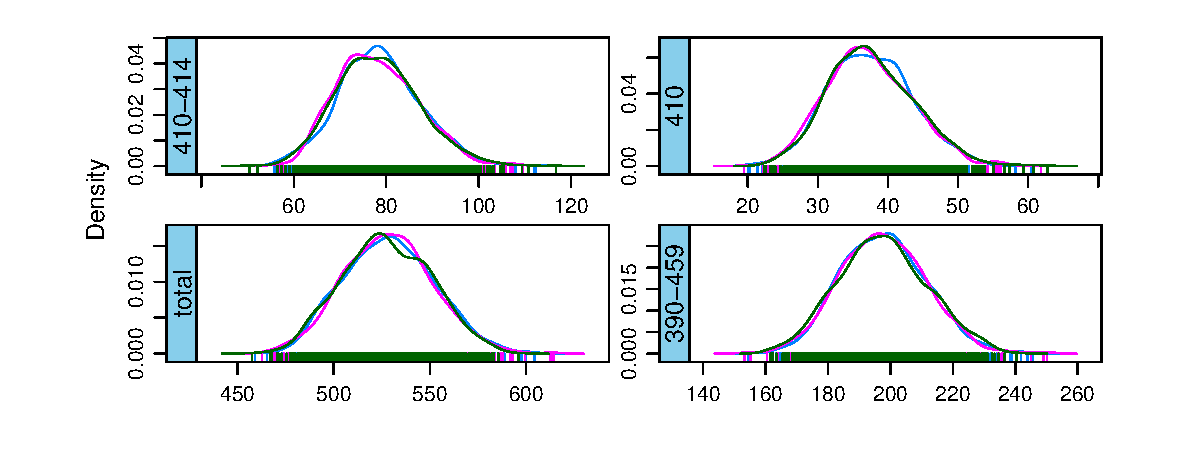
\includegraphics[width=1\linewidth]{../../R-codes/JAGS/plots/mimic/Density410h}
	\caption{Posterior distributions for ICD 410 and its ancestors, with added anomalies, and calculated with Hierarchiacl Bayes model}
	\label{fig:density410h}
\end{figure}

Table~\ref{tab:postsum410.mimic} and figure~\ref{fig:density410} shows the posterior for IBM and table~\ref{tab:postsum410h.mimic} and figure~\ref{fig:density410h} shows the posterior for HBM, for ICD 410 and its ancestors, with added anomalies. There are is an obvious differences (more than double at leaf) between the distribution values and distribution shape for IBM and HBM. 

\newpage%----------------------------------- 415 -------------------------------------------

\begin{table}[!t]
	\centering
	\begin{tabular}{rrrrrrrr}
		\hline
		& mean & sd & 2.5\% & 50\% & 97.5\% & Rhat & n.eff \\ 
		\hline
		total & 528.937 & 23.037 & 484.629 & 528.703 & 574.379 & 1.000 & 2859.000 \\ 
		390-459 & 198.553 & 14.315 & 171.867 & 198.445 & 227.649 & 1.000 & 3000.000 \\ 
		415-417 & 6.364 & 2.494 & 2.470 & 6.059 & 11.999 & 1.000 & 2419.000 \\ 
		415 & 6.436 & 2.571 & 2.373 & 6.117 & 12.070 & 1.000 & 2139.000 \\ 
		\hline
	\end{tabular}
	\caption{Posterior distributions for ICD 415 and its ancestors, with added anomalies, and calculated with independent Bayes model} 
	\label{tab:postsum415.mimic}
\end{table}

\begin{figure}[!h]
	\centering
	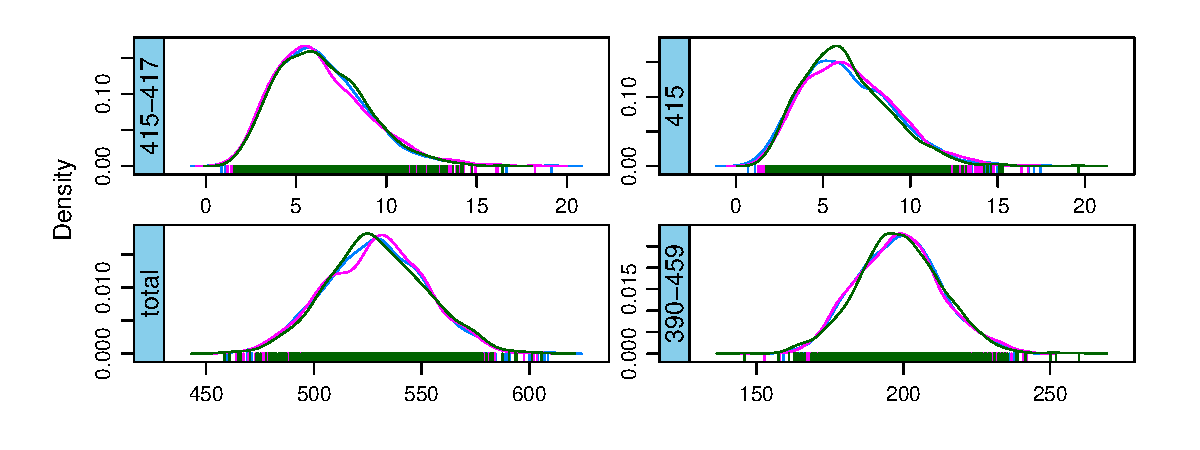
\includegraphics[width=1\linewidth]{../../R-codes/JAGS/plots/mimic/Density415}
	\caption{Posterior distributions for ICD 415 and its ancestors, with added anomalies, and calculated with independent Bayes model}
	\label{fig:density415}
\end{figure}

\newpage%----------------------------------- 415 H -------------------------------------------

\begin{table}[!t]
	\centering
	\begin{tabular}{rrrrrrrr}
		\hline
		& mean & sd & 2.5\% & 50\% & 97.5\% & Rhat & n.eff \\ 
		\hline
		total & 526.519 & 23.086 & 481.720 & 526.254 & 572.876 & 1.000 & 3000.000 \\ 
		390-459 & 195.702 & 13.884 & 169.817 & 195.471 & 223.270 & 1.000 & 3165.000 \\ 
		415-417 & 3.146 & 1.784 & 0.721 & 2.827 & 7.459 & 1.000 & 1876.000 \\ 
		415 & 3.308 & 1.953 & 0.680 & 2.942 & 7.934 & 1.000 & 1730.000 \\ 
		\hline
	\end{tabular}
	\caption{Posterior distributions for ICD 415 and its ancestors, with added anomalies, and calculated with Hierarchical Bayes model} 
	\label{tab:postsum415h.mimic}
\end{table}

\begin{figure}[!h]
	\centering
	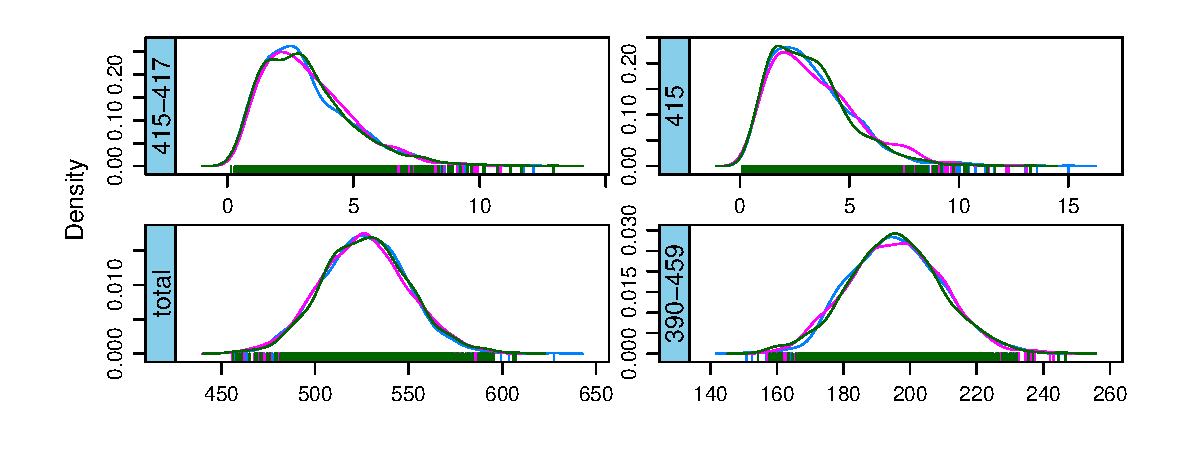
\includegraphics[width=1\linewidth]{../../R-codes/JAGS/plots/mimic/Density415h}
	\caption{Posterior distributions for ICD 415 and its ancestors, with added anomalies, and calculated with Hierarchical Bayes model}
	\label{fig:density415h}
\end{figure}

Table~\ref{tab:postsum415.mimic} and figure~\ref{fig:density415} shows the posterior for IBM and table~\ref{tab:postsum415h.mimic} and figure~\ref{fig:density415h} shows the posterior for HBM, for ICD 415 and its ancestors, with added anomalies. There are is an obvious differences (almost double at leaf) between the distribution values and distribution shape for IBM and HBM.

\newpage%----------------------------------- 452 -------------------------------------------

\begin{table}[!t]
	\centering
	\begin{tabular}{rrrrrrrr}
		\hline
		& mean & sd & 2.5\% & 50\% & 97.5\% & Rhat & n.eff \\ 
		\hline
		total & 526.983 & 23.297 & 480.980 & 526.758 & 573.138 & 1.000 & 3114.000 \\ 
		390-459 & 196.224 & 13.951 & 169.986 & 195.689 & 224.270 & 1.000 & 3294.000 \\ 
		451-459 & 7.382 & 2.629 & 3.052 & 7.077 & 13.190 & 1.000 & 2322.000 \\ 
		452 & 0.346 & 0.208 & 0.033 & 0.323 & 0.812 & 1.000 & 517.000 \\ 
		\hline
	\end{tabular}
	\caption{Posterior distributions for ICD 452 and its ancestors, with added anomalies, and calculated with independent Bayes model} 
	\label{tab:postsum452.mimic}
\end{table}

\begin{figure}[!h]
	\centering
	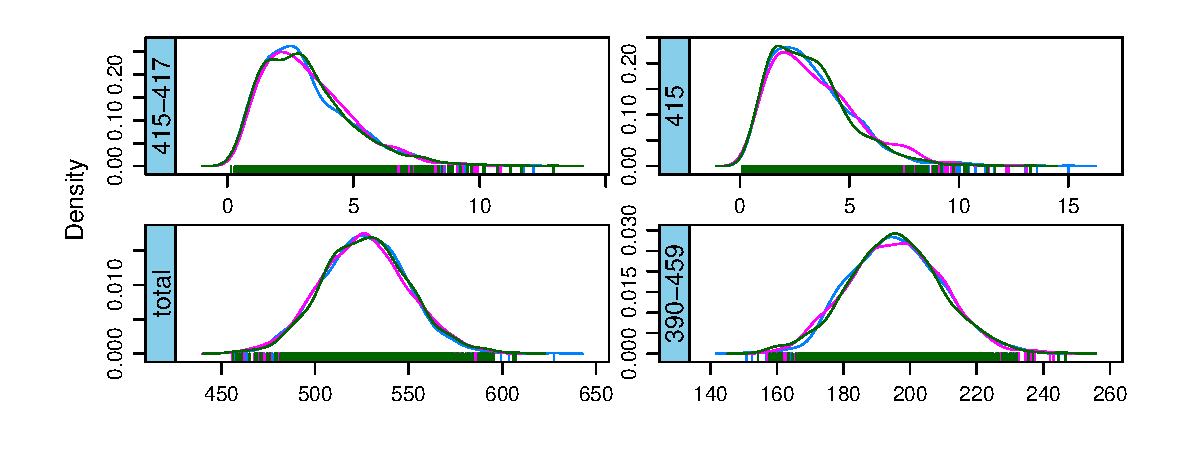
\includegraphics[width=1\linewidth]{../../R-codes/JAGS/plots/mimic/Density415h}
	\caption{Posterior distributions for ICD 452 and its ancestors, with added anomalies, and calculated with independent Bayes model}
	\label{fig:density452}
\end{figure}

\newpage%----------------------------------- 452 H -------------------------------------------

\begin{table}[!t]
	\centering
	\begin{tabular}{rrrrrrrr}
		\hline
		& mean & sd & 2.5\% & 50\% & 97.5\% & Rhat & n.eff \\ 
		\hline
		total & 526.447 & 23.045 & 482.679 & 526.250 & 572.946 & 1.000 & 3061.000 \\ 
		390-459 & 195.096 & 13.618 & 168.448 & 194.678 & 222.373 & 1.000 & 2950.000 \\ 
		451-459 & 7.476 & 2.495 & 3.299 & 7.282 & 13.055 & 1.000 & 1358.000 \\ 
		452 & 0.390 & 0.222 & 0.045 & 0.362 & 0.889 & 1.020 & 342.000 \\ 
		\hline
	\end{tabular}
	\caption{Posterior distributions for ICD 452 and its ancestors, with added anomalies, and calculated with Hierarchical Bayes model} 
	\label{tab:postsum452h.mimic}
\end{table}

\begin{figure}[!h]
	\centering
	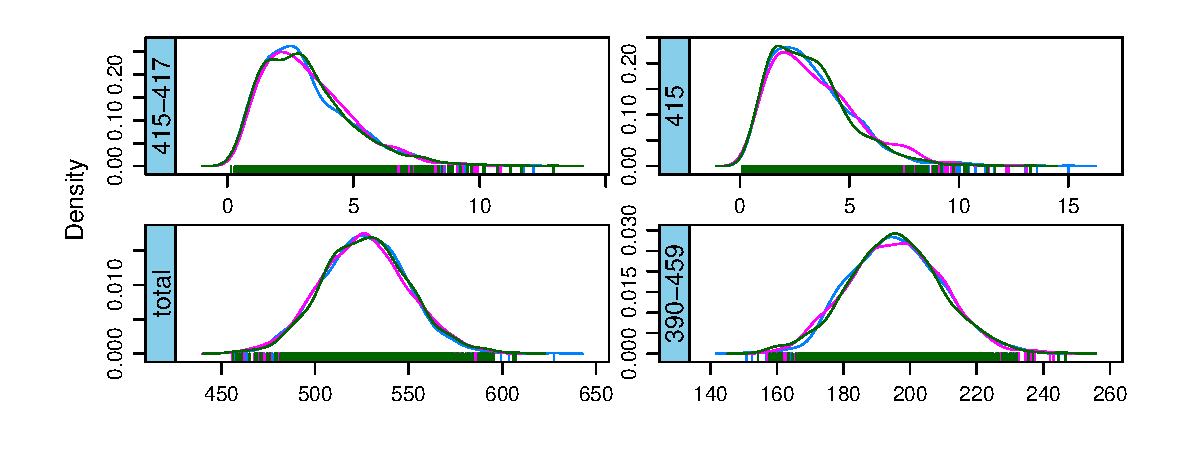
\includegraphics[width=1\linewidth]{../../R-codes/JAGS/plots/mimic/Density415h}
	\caption{Posterior distributions for ICD 452 and its ancestors, with added anomalies, and calculated with Hierarchical Bayes model}
	\label{fig:density452h}
\end{figure}

Table~\ref{tab:postsum452.mimic} and figure~\ref{fig:density452} shows the posterior for IBM and table~\ref{tab:postsum452h.mimic} and figure~\ref{fig:density452h} shows the posterior for HBM, for ICD 452 and its ancestors, with added anomalies. There are no obvious differences between the distribution values and distribution shape for IBM and HBM.

\newpage %----------------------------- all ----------------------------------    

\begin{figure}[!h]
	\centering
	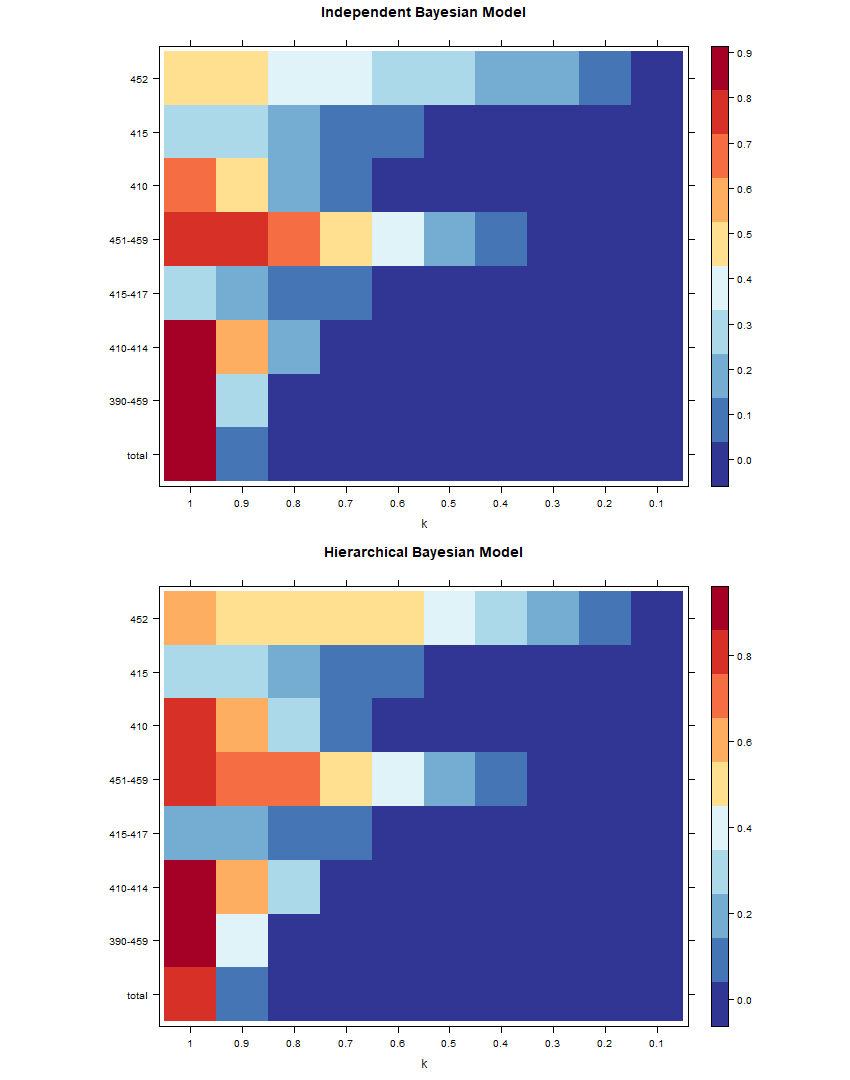
\includegraphics[width=1\linewidth]{../../R-codes/JAGS/plots/mimic/heatnorm}
	\caption{Heat-map of anomaly signals for ICD 410,415 and 452 and its ancestors, with no added anomalies, of IBM and HBM.}
	\label{fig:heatnorm}
\end{figure}

\newpage

\begin{figure}[!h]
	\centering
	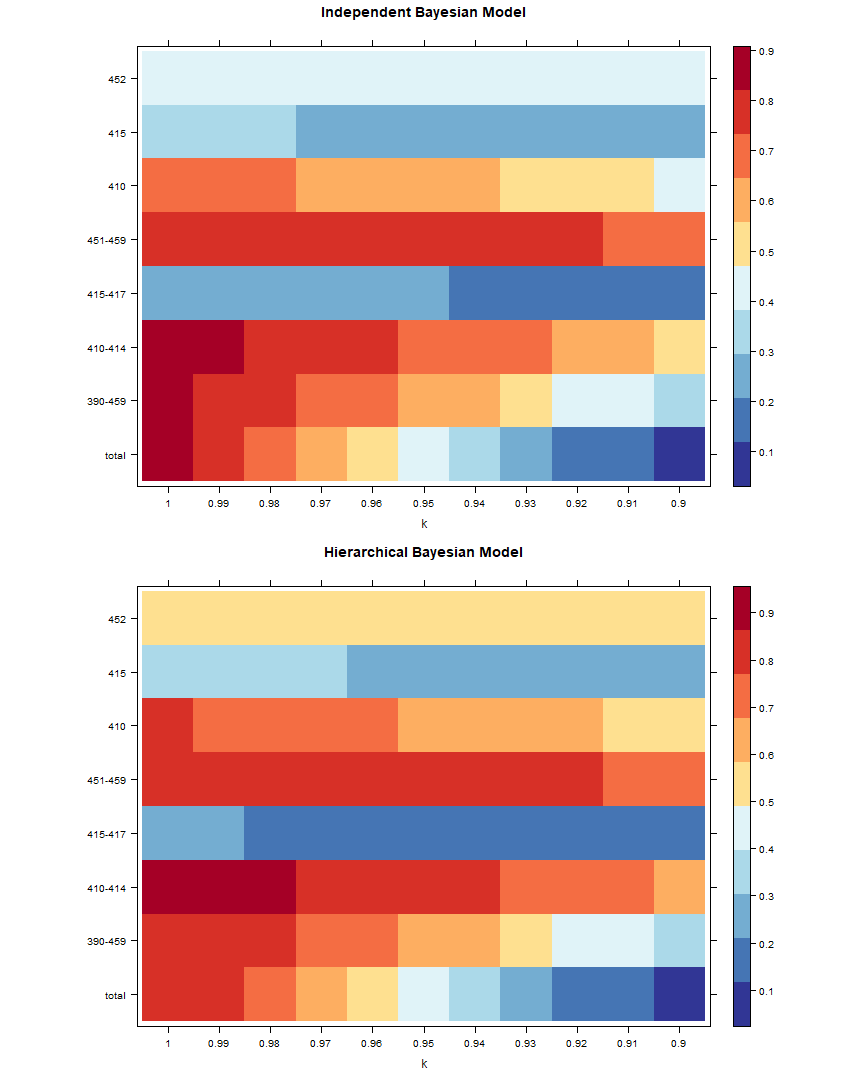
\includegraphics[width=1\linewidth]{../../R-codes/JAGS/plots/mimic/heatnorm2}
	\caption{Heat-map of anomaly signals for ICD 410,415 and 452 and their ancestors, with no added anomalies, of IBM and HBM zoomed in at k values of 0.9 to 1.}
	\label{fig:heatnorm2}
\end{figure}

\newpage

The heat-map in figure~\ref{fig:heatnorm} presents the anomaly signals of ICD 410,415 and 452 and their ancestors with no addition of a constant anomaly, with IBM and HBM, against different increments of $k$.Anomaly signals tend to be stronger as k increase, and stronger for lower hierarchies compare to higher hierarchies, the variability of signal strength also tend to increase with higher hierarchy. Zooming in at looking at k values from 0.6 to 1 in figure~\ref{fig:heatnorm2}, we observe a noticeable small difference in anomaly detection rate between IBM and HBM for category AA. Our observation suggests that the difference between anomaly detection rate is small or close to none for IBM and HBM, on the bottom of the hierarchy, for anomaly with a different hierarchical structure, in a simulated setting with each category generated independently.   

\newpage%----------------------------- 410 ----------------------------------

\begin{figure}[!h]
	\centering
	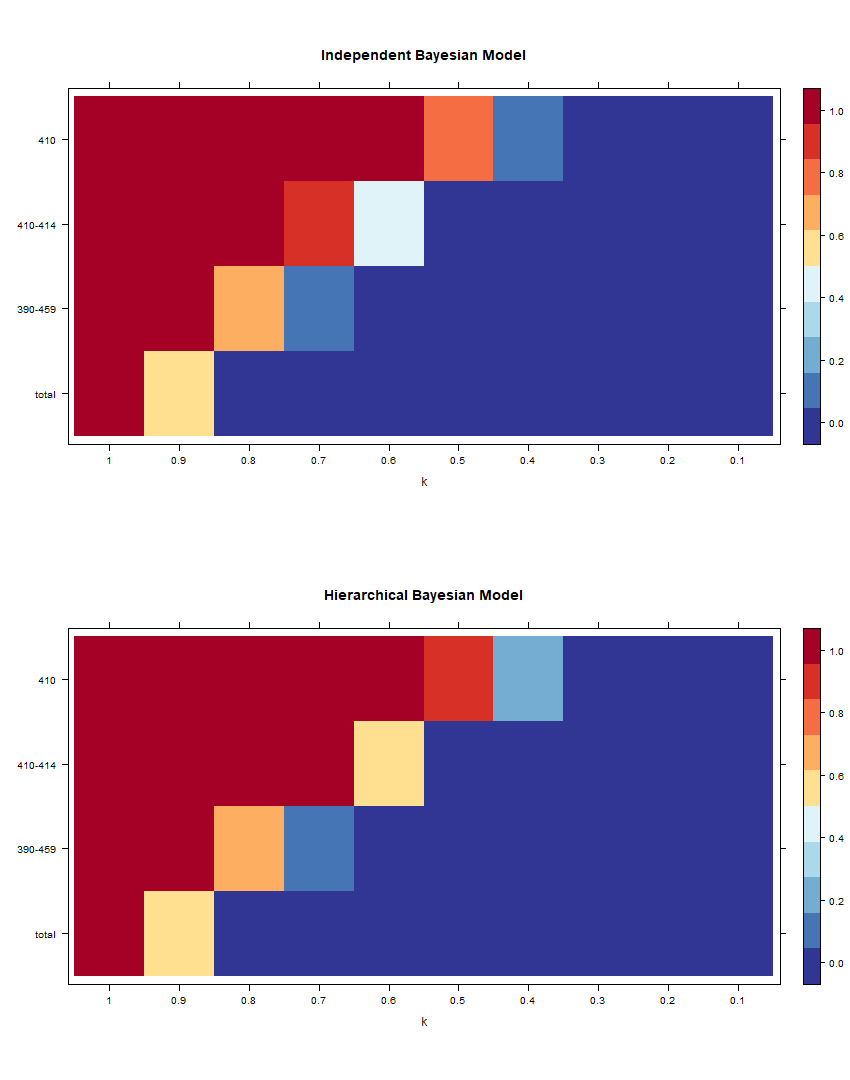
\includegraphics[width=1\linewidth]{../../R-codes/JAGS/plots/mimic/heat410}
	\caption{Heat-map of anomaly signals for ICD 410 and its ancestors, with no added anomalies, of IBM and HBM.}
	\label{fig:heat410}
\end{figure}

\newpage

\begin{figure}[!h]
	\centering
	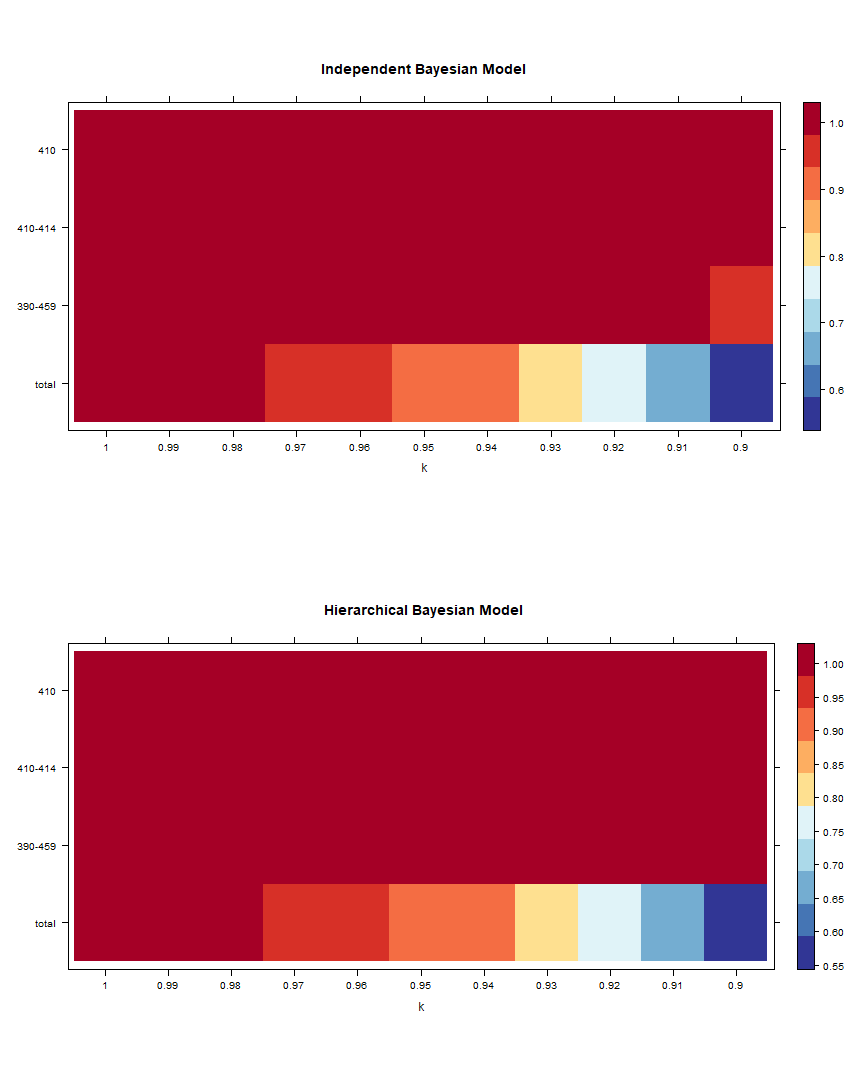
\includegraphics[width=1\linewidth]{../../R-codes/JAGS/plots/mimic/heat4102}
	\caption{Heat-map of anomaly signals for ICD 410 and its ancestors, with no added anomalies, of IBM and HBM zoomed in at k values of 0.9 to 1.}
	\label{fig:heat4102}
\end{figure}

\newpage

The heat-map in figure~\ref{fig:heat410} presents the anomaly signals of ICD 410 and their ancestors with no addition of a constant anomaly, with IBM and HBM, against different increments of $k$.Anomaly signals tend to be strong on the top left of the heat map. This suggests that signals of anomaly tend to increase in strength with increased k and higher hierarchy. Zooming in at looking at k values from 0.6 to 1 in figure~\ref{fig:heat4102}, we observe a noticeable small difference in anomaly detection rate between IBM and HBM for category AA. Our observation suggests that the difference between anomaly detection rate is small or close to none for IBM and HBM, on the bottom of the hierarchy, for anomaly with a different hierarchical structure, in a simulated setting with each category generated independently. 

\newpage%----------------------------- 415 ----------------------------------

\begin{figure}[!h]
	\centering
	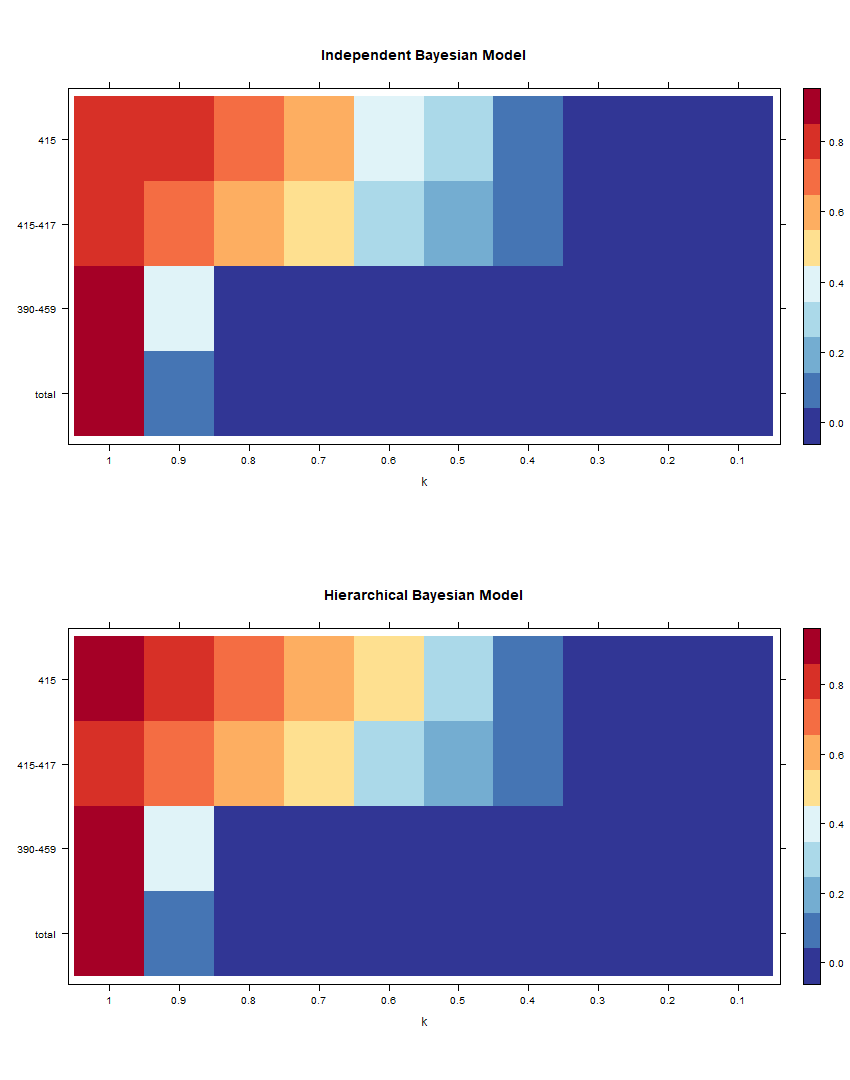
\includegraphics[width=1\linewidth]{../../R-codes/JAGS/plots/mimic/heat415}
	\caption{Heat-map of anomaly signals for ICD 415 and its ancestors, with no added anomalies, of IBM and HBM.}
	\label{fig:heat415}
\end{figure}

\newpage

\begin{figure}[!h]
	\centering
	\includegraphics[width=1\linewidth]{../../R-codes/JAGS/plots/mimic/heat4152}
	\caption{Heat-map of anomaly signals for ICD 415 and its ancestors, with no added anomalies, of IBM and HBM zoomed in at k values of 0.9 to 1.}
	\label{fig:heat4152}
\end{figure}

\newpage

The heat-map in figure~\ref{fig:heat415} presents the anomaly signals of ICD 415 and their ancestors with no addition of a constant anomaly, with IBM and HBM, against different increments of $k$.Anomaly signals tend to be strong on the top left of the heat map. This suggests that signals of anomaly tend to increase in strength with increased k and higher hierarchy. Zooming in at looking at k values from 0.6 to 1 in figure~\ref{fig:heat4152}, we observe a noticeable small difference in anomaly detection rate between IBM and HBM for category AA. Our observation suggests that the difference between anomaly detection rate is small or close to none for IBM and HBM, on the bottom of the hierarchy, for anomaly with a different hierarchical structure, in a simulated setting with each category generated independently.

\newpage%----------------------------- 452 ----------------------------------

\begin{figure}[!h]
	\centering
	\includegraphics[width=1\linewidth]{../../R-codes/JAGS/plots/mimic/heat452}
	\caption{Heat-map of anomaly signals for ICD 452 and its ancestors, with no added anomalies, of IBM and HBM.}
	\label{fig:heat452}
\end{figure}

\newpage

\begin{figure}[!h]
	\centering
	\includegraphics[width=1\linewidth]{../../R-codes/JAGS/plots/mimic/heat4522}
	\caption{Heat-map of anomaly signals for ICD 452 and its ancestors, with no added anomalies, of IBM and HBM zoomed in at k values of 0.9 to 1.}
	\label{fig:heat4522}
\end{figure}

\newpage

The heat-map in figure~\ref{fig:heat452} presents the anomaly signals of ICD  452 and their ancestors with no addition of a constant anomaly, with IBM and HBM, against different increments of $k$. Anomaly signals tend to be strong on the top left of the heat map. This suggests that signals of anomaly tend to increase in strength with increased k and higher hierarchy. Zooming in at looking at k values from 0.6 to 1 in figure~\ref{fig:heat4522}, we observe a noticeable small difference in anomaly detection rate between IBM and HBM for category AA. Our observation suggests that the difference between anomaly detection rate is small or close to none for IBM and HBM, on the bottom of the hierarchy, for anomaly with a different hierarchical structure, in a simulated setting with each category generated independently.

\newpara

There are significant differences in anomaly signals of disease categories with different rate of occurrence. For common diseases (ICD 410)the signals seem to be more clear (change in colour for different increments of $k$ is more abrupt) compare to rare (ICD 415) and extremely rare (ICD 452)disease categories. Signals seem to exist for categories at level 3 readily and level 2 of the hierarchy, for commonly diseases signals can be observed in level 1, but for rare and extremely rare diseases there is almost no signal at level 1. Signals at level 2 seem to be weaker than signals at level 3 overall, but it is still apparent and easily detectable.  

\section{Discussion}

We were unable to make a conclusion for the goodness-of-fit comparison between IBM and HBM because the mean and median values of differences in DIC are very close to 0. This suggests that for real-life data with large complex hierarchical structures, IBM and HBM performed very similarly. The finding is unexpected, as our simulation studies and several academic papers all seem to have suggested HBM be the superior model. There are several possible explanations for this. The first explanation is that for large complex hierarchical structures there are a huge amount of categories at each of the levels, and randomness from all these categories could have masked the small improvements in the goodness of fit for anomalies at one small category. Also that our HBM are quite primitive and there is no way for us to know whether or it really captures the hierarchical relationship, and the validity of our HBM is in question. If our HBM does not capture the hierarchical structure information, then there will not be any reason that HBM performs IBM. We also made observations that, for an extremely rare disease, the posterior distribution is not normal an seem to be skewed, but our model assumes it to be normal. We could possibly use different priors for categories with different magnitude of counts, for example, assigning a Half-Cauchy prior that was suggested by \citet{gelman2006prior} for extremely rare categories. 

\newpara

The mean of posterior distribution of disease with different prevalence of occurrence using IBM and HBM yield significant differences, with IBM yielding larger mean. For common disease the difference at leaf level is large, less common the less the difference, with uncommon disease there are almost no noticeable difference. This happens because for IBM, there are no information about the hierarchical structure that constraint the convergence in the MCMC process, thus a single abnormal observation have a greater influence on the posterior. And for HBM, the hierarchical structure meant that we are considering more than just the leaf level, but other higher levels as well.  

\newpara

There are significant differences in anomaly signals of disease categories with different rate of occurrence. We noticed that for common disease category signals of the anomaly are still visible at level 1 of the hierarchy, but for rare and extremely are disease categories, there is almost no signal. However, signals can still be readily observed at level 2 and level 3 of the hierarchy for rare and extremely rare disease categories. Our observation made sense because rare and common disease have a much smaller magnitude of counts and as lower hierarchy aggregate into a higher hierarchy, smaller counts tend to get masked by randomness and uncertainty from other categories, so it would become harder to detect the anomaly at higher hierarchy levels. For ICD-9 disease categories, we are able to detect anomaly at the bottom two levels. This suggests that we should not look at anomaly at level 1 of hierarchy because we are likely to miss it. The rarity of disease also have a significant impact on anomaly detection, for common disease with large average values, signals of the anomaly are clear and easy to detect, but for rare and extremely rare disease categories it is unclear and harder to decide.

\newpara

Overall we see that if the capacity is under 60\% ish, there are almost no anomaly signal, this meant that if the hospitals are operating at capacities at or under 60\%, they will almost never exceed their full capacity even if there are twice as many arrivals for certain disease categories compare to usual. It is a bit hard to make sense of this, but essentially what you need to know is that operating at a lower capacity should have a significant impact on the likelihood of anomalous arrivals. The obvious solution to congestion is to decrease the operation capacity (or increase overall capacity), but this is easier said than been done because the hospitals would have done it if they could. However, our results still high lighted the fact that having a lower operation capacity could effectively buffer against anomalous events and reduce the likelihood of congestion from occurring. 
	
	

%	\chapter{Gene Ontology}\label{chap:Jellyfish}

A hierarchical structure is also frequently seen in genetics data, Gene Ontology (GO) groups different genes into a multi-domain hierarchical network \citep{GO2007}, which is a representation of genetic relationship and network of significant GO categories often serve as a basis for genetic analyses.
Molecular dissection of box jellyfish venom cytotoxicity highlights an effective venom antidote
\section{Introduction}

\section{Gene set enrichment analysis}
\section{title}
\section{title}
\section{title}

\citet{lau2019molecular}

\begin{landscape}
	...
\end{landscape}

% https://tex.stackexchange.com/questions/182896/setting-up-apa-tables-three-problems
\newpage
\begin{landscape}
\begin{table}[htp]
	\centering
	\addtolength{\tabcolsep}{3pt} % some more room between columns
	
	\caption{Group Example}
	
	\begin{tabular}{
			l
			S[table-format=2.0]
			S[table-format=2.1]
			S[table-format=1.1]
			S[table-format=-1.2]
			S[table-format=.2,table-comparator=true]
		}
		\toprule
		Variable & {$n$} & {$M$} & {$\mathit{SD}$} & {$t$} & {$p$} \\
		\midrule
		Overall group  &    &      &     & -3.43 & <0.01 \\
		\IE Group A    & 20 & 10.3 & 4.3 \\
		\IE Group B    & 30 & 14.3 & 1.4 \\
		\addlinespace
		Sex \\
		\IE Female     &    &      &     & -3.43 & <0.01 \\
		\IE[2] Group A & 10 & 10.3 & 4.3 \\
		\IE[2] Group B & 15 & 14.3 & 1.4 \\
		\IE Male       &    &      &     & -3.43 & <0.01 \\
		\IE[2] Group A & 10 & 10.3 & 4.3 \\
		\IE[2] Group B & 15 & 14.3 & 1.4 \\
		\midrule[\heavyrulewidth]
		\multicolumn{6}{l}{$M=\text{mean}$, $\mathit{SD}=\text{standard deviation}$}
	\end{tabular}
	
\end{table}

\begin{table}[htpb]
		\centering
	\caption{The caption of the table.}
	\begin{tabular}{cccc}
		\toprule
		Column 1 & \multicolumn{3}{c}{Column 2} \\
		& Column 2a & Column 2b & Column2c \\
		\midrule
		1 & 1 & .67 & 5 \\
		1 & 2 & .32 & 2 \\
		1 & 3 & .01 & 4 \\
		\bottomrule
	\end{tabular}
	
	\bigskip
	\small\textit{Note}. The caption should now be correctly formatted.
\end{table}


\end{landscape}

\newpage
ffff

%	\chapter{Discussion}





The Ecological fallacy refers to inference about individuals based on analyses of group data. In such instance, individual characteristic are masked by the group average and it becomes harder to distinguish individual characteristics \citep{herring2001culture}. The same 






\section{1 stage Hierarchiacl Poisson model}

	\begin{equation}\nonumber
	y \sim Poisson(\mu) \;\;\; then \;\;\; E(y) = var(y) =\mu
	\end{equation}
	
	JAGS code




\section{2 stage Hierarchiacl Poisson model}

	\begin{equation}\nonumber
	y_T \sim Poisson(\sum_{i=1}^{N_i} \mu_i) 
	\end{equation}

	\begin{equation}\nonumber
	y_i \sim Poisson(\mu_i) 
	\end{equation}

	\begin{equation}\nonumber
	\mu_i \sim Gamma(\alpha,\beta) 
	\end{equation}

	Prior for the hyperparameters

	\begin{equation}\nonumber
	\alpha \sim Gamma(a,b) 
	\end{equation}

	\begin{equation}\nonumber
	\beta \sim Gamma(c,d) 
	\end{equation}
	
\section{3 stage Hierarchiacl Poisson model}

	\begin{equation}\nonumber
	y_T \sim Poisson(\sum_{i=1}^{N_i} \sum_{j=1}^{N_j}\mu_{ij}) 
	\end{equation}

	\begin{equation}\nonumber
	y_i \sim Poisson( \sum_{j=1}^{N_j}\mu_{j}) 
	\end{equation}
	
	\begin{equation}\nonumber
	y_{ij} \sim Poisson(\mu_{ij}) 
	\end{equation}

	\begin{equation}\nonumber
	\mu_{ij} \sim Gamma(\alpha,\beta) 
	\end{equation}

	Prior for the hyperparameters

	\begin{equation}\nonumber
	\alpha \sim Gamma(a_{ij},b_{ij}) 
	\end{equation}

	\begin{equation}\nonumber
	\beta \sim Gamma(c_{ij},d_{ij}) 
	\end{equation}
	
	Prior for the hyper-hyperparameters

	\begin{equation}\nonumber
	\alpha \sim Gamma(a_{ij},b_{ij}) 
	\end{equation}

	\begin{equation}\nonumber
	\beta \sim Gamma(c_{ij},d_{ij}) 
	\end{equation}

Notes

\begin{equation*}
y_i = \{y_A,y_B\}
\end{equation*}

\begin{equation*}
y_{ij} = \{y_{AA},y_{AB},y_{BA},y_{BB}\}
\end{equation*}

\begin{equation*}
\beta \sim Gamma(c_{ij},d_{ij}) 
\end{equation*}

\begin{equation*}
y_{t}=y_{AA,t}+y_{AB,t}+y_{BA,t}+y_{BB,t}.
\end{equation*}

\begin{equation*} y_{A,t}=y_{AA}{t}+y_{AB,t}\quad \quad y_{B,t}=y_{BA,t}+y_{BB,t}
\tag{10.4}
\end{equation*}

\section{Hierarchical Poisson regression models}
\section{Hierarchical timeseries models}


\section{Hierarchical Poisson timeseries models}


\begin{equation*}
\end{equation*}


\begin{figure}[!h]
	\centering
	\begin{tabular}{cc}
		\subf{\includegraphics[width=65mm]{../../R-codes/Simulation/plot/anomaly/ggdaily1S10leaf}}
		{Anomaly$=10$}
		&
		\subf{\includegraphics[width=65mm]{../../R-codes/Simulation/plot/anomaly/ggdaily1S25leaf}}
		{Anomaly$=2$}
		\\
		\subf{\includegraphics[width=65mm]{../../R-codes/Simulation/plot/anomaly/ggdaily1S50leaf}}
		{Anomaly$=50$}
		&
		\subf{\includegraphics[width=65mm]{../../R-codes/Simulation/plot/anomaly/ggdaily1S100leaf}}
		{Anomaly$=100$}
		\\
		\subf{\includegraphics[width=65mm]{../../R-codes/Simulation/plot/anomaly/ggdaily1S250leaf}}
		{Anomaly'$=250$}
		&
		\subf{\includegraphics[width=65mm]{../../R-codes/Simulation/plot/anomaly/ggdaily1S500leaf}}
		{Anomaly $=500$}
		\\
	\end{tabular}
	\caption{Visual inspection of different increment of anomalies at level 2 of hierarchy}
	\label{fig:addanomleaf}
\end{figure}

\newpage %------------------------------------------------------------------------------------------    
\begin{figure}[!h]
	\centering
	\begin{tabular}{cc}
		\subf{\includegraphics[width=65mm]{../../R-codes/Simulation/plot/anomaly/ggdaily1S10B1}}
		{Anomaly$=10$}
		&
		\subf{\includegraphics[width=65mm]{../../R-codes/Simulation/plot/anomaly/ggdaily1S25B1}}
		{Anomaly$=2$}
		\\
		\subf{\includegraphics[width=65mm]{../../R-codes/Simulation/plot/anomaly/ggdaily1S50B1}}
		{Anomaly$=50$}
		&
		\subf{\includegraphics[width=65mm]{../../R-codes/Simulation/plot/anomaly/ggdaily1S100B1}}
		{Anomaly$=100$}
		\\
		\subf{\includegraphics[width=65mm]{../../R-codes/Simulation/plot/anomaly/ggdaily1S250B1}}
		{Anomaly'$=250$}
		&
		\subf{\includegraphics[width=65mm]{../../R-codes/Simulation/plot/anomaly/ggdaily1S500B1}}
		{Anomaly $=500$}
		\\
	\end{tabular}
	\caption{Visual inspection of different increment of anomalies at level 1 of hierarchy}
	\label{fig:addanomB1}
\end{figure}



% 	\chapter{Conclusions}

	the size definition of point anomaly and  period anomaly used are

$	if mu_pointanomaly = 100, size of point anomaly will be 100, however for period anomaly, mu_period anomaly is the highest point, and not the sum total count through out the period. the distribution of period anomaly will influence the size of each day.  $

for example, 

List of simulated data used can be found in appendix ref

name  simulation  anomaly

6 Note 1000 sample did not give stable dic, try 10000


t.start = "2006/01/01 00:00:01"   
t.end = "2018/12/31 23:59:59"
100000

matrix1 = cbind(            
c(100,100),                 
c(100,100))

\begin{table}[ht]
	\centering
	\begin{tabular}{rrrrrrr}
		\hline
		N & st & et & \text{cat2.val}  & output file\\ 
		\hline
		100000 & "2006/01/01 00:00:01" & "2018/12/31 23:59:59" & matrix1 & raw1.df \\ 
		100000 & "2006/01/01 00:00:01" & "2018/12/31 23:59:59" & matrix2 & raw2.df \\ 
		100000 & "2006/01/01 00:00:01" & "2018/12/31 23:59:59" & matrix3 & raw3.df \\ 
		100000 & "2006/01/01 00:00:01" & "2018/12/31 23:59:59" & matrix4 & raw4.df \\ 
		\hline
	\end{tabular}
	\caption{Function settings for synthetic data used in section XXX}
\end{table}
% 	\chapter{Conclusions}

	the size definition of point anomaly and  period anomaly used are

$	if mu_pointanomaly = 100, size of point anomaly will be 100, however for period anomaly, mu_period anomaly is the highest point, and not the sum total count through out the period. the distribution of period anomaly will influence the size of each day.  $

for example, 

List of simulated data used can be found in appendix ref

name  simulation  anomaly

6 Note 1000 sample did not give stable dic, try 10000


t.start = "2006/01/01 00:00:01"   
t.end = "2018/12/31 23:59:59"
100000

matrix1 = cbind(            
c(100,100),                 
c(100,100))

\begin{table}[ht]
	\centering
	\begin{tabular}{rrrrrrr}
		\hline
		N & st & et & \text{cat2.val}  & output file\\ 
		\hline
		100000 & "2006/01/01 00:00:01" & "2018/12/31 23:59:59" & matrix1 & raw1.df \\ 
		100000 & "2006/01/01 00:00:01" & "2018/12/31 23:59:59" & matrix2 & raw2.df \\ 
		100000 & "2006/01/01 00:00:01" & "2018/12/31 23:59:59" & matrix3 & raw3.df \\ 
		100000 & "2006/01/01 00:00:01" & "2018/12/31 23:59:59" & matrix4 & raw4.df \\ 
		\hline
	\end{tabular}
	\caption{Function settings for synthetic data used in section XXX}
\end{table}
	
\chapter{Conclusion} \label{chap:Conclusion1}

\section{Introduction}

For this thesis we ran several simulations that explore the performance of Hierarchical Bayesian Model (HBM) over the Independent Bayesian Model(IBM). We also investigated whether taking existing hierarchical structures in ICD-9 disease diagnoses codes into account would affect the anomaly signal for different occurrence levels of disease diagnoses. In this chapter, the findings from this thesis are summarised and discussed, extensions on our methodology and potential directions for future research are discussed.

\section{Summary of findings}

Models that used weakly-informed priors had outperformed the model with non-informative prior, in terms of model goodness-of-fit. Assignment of prior is a prerequisite of a quality model, without any prior results of our Bayesian model will differ with models that have a prior by an substantial amount. However, small differences in the distribution of the prior does not create noticeable differences, therefore we have great freedom in what prior to use. There are number of suggestion by academics in the field such as Gilman and most are fairly robust and feasible options. 

\newpara

size of the anomalies have strong association with several posterior values. Increase of size of anomaly will decrease number of Effective Sample Size (ESS), and increase the size of standard deviation. This is mostly due to how the relative size of values differ for large and small values. Due to the aggregation constraint there are usually significant difference in size for different levels of hierarchy, higher the hierarchy the larger the mean size. For such reasons, when we are dealing with hierarchical datasets, we must take into account the hierarchical structure otherwise power of our models will be greatly reduced. There are more information at lower levels of the hierarchy, therefore when informations about hierarchical structure is disregarded, the lower level of hierarchy often result in greatest differences between IBM and HBM.  

\newpara

For real-life datasets with complex hierarchical structures it was very difficult to prove superiority of HBM over IBM, and hence no conclusions can be made. there are several possible reasons that might contribute to the difficulty, such as uncertainty, and the validity of the HBM used. There are significant differences in anomaly signals of disease categories with different rate of occurrence. for more common diseases it will have greater impact on the higher hierarchy and there maybe signals from level 3 to level 1, for rare and extremely rare cases we could not detect anomaly at level 1 and can only detect anomaly ay level 2 to level 3. There seem to be a dissipating effect, that anomalies occur at a level will lose it's presences, for levels further away from the original level. Of course, this is due to aggregation of other groups masking the anomaly with their noise. For smaller categories dissipation effect are stronger.

\section{Extensions on Methodology}


Hierarchical time-series techniques have worked fairly well for our studies, some of the down side is that the time-consumliess of the process and that the optimally reconciliation algorithm gives negative results. Unfortunately function for non-negative optimal reconciliation prediction will not be implemented until after the submission of the thesis. 

Uncertainty in Bayesian estimations has certainly add difficulties to the processes of model selections and result exploration. Uncertainty is a strength and a weakness of Bayesian inference, in our case difference in DIC are sometimes hard to distinguish, and we were unable to made strong claims to our findings   Also with increased parameter that contained uncertainty, the computational cost increases dramatically with the increase in dimensionality, and limits the practicality. For simple models the problems isn't so bad, but with large complex data, running models may take hours and hours, and we often cannot make significant observations from results.    

\section{Implications}

A possible implications of our work is to create an online signal detection alarm system that raises an alarm that notifies hospital management of congestion when and before it occurs, and models the possibility of abnormally high arrivals. With all the development in big data, data linkage and data streaming, there is enough resource for this idea to start in development in a practical setting. The idea is that by collecting data from various sources and send them to an online cloud platform, that integrates this information on arrival and exports signals of anomalies for different locations. If an alarm is raised at a location, steps could be taken at the earliest instance to deal with the problem. The essence of the idea is to detect and deal with the problem before it occurs.  It does not take any effort to call for interference if congestion happened at a location, but this takes time and human, and by the time the problem is noticed, and the message got through to management, the negative effect would already be in effect. The system would, in theory, improve the efficiency of operation and reduce the chance of congestion of happening. 

\newpara

Another possible practical application of our techniques is to disaggregate the geo-location attribute from the New Zealand National Minimum Dataset (NMDS) data and try to monitor the anomalies for a geo-location hierarchy. Information analyst from the Ministry of Health has suggested that anomalies in health data are often due to differences in patient management strategies for different District Health Boards(DHB) from different parts of the country. For example, is there an after-hours clinic available or is the hospital the only available treatment provider? Alternatively, does this DHB manage patients by transferring them through different facilities or does it all take place in one facility (albeit potentially covering different sites)?  Modelling and identifying anomalies at the individual doctor level, department level, individual facility level, DHB level, and island level with HBM could provide statistical evidence about how each doctor department, facility and DHB in New Zealand is performing independently and collectively. If a particular department always shows signals of abnormal arrivals, it could suggest that the department is operating at near full capacity and this particular department need more doctors and staff. If a high anomaly at particular DHB is observed, only in the evening, maybe an overall lack of staff for the after-hour clinic is the cause and roaster needs to be adjusted. The main idea is that observations of anomalies could translate into problematic operations and our HBM techniques have a significant advantage to, especially in small and time-related anomalies that are hard to detect by the intuition of hospital management, and informed decisions can be made to improve the current system and alleviate the problem of congestion. 

\section{Future Directions}

Future work will be aimed to extend the scope of the current simulations. For our exploratory analysis, HBM has shown to have superior performance over IBM, we could still think of other settings that could also test the robustness of HBM with datasets with different qualities, and evaluate the performance of HBM from different perspectives
of data. For example We could increase the number of levels of hierarchy, and see how HBM perform with data with increasing complexity. We could try and test for hierarchical networks that do not necessarily follow the aggregation constraint, and see how HBM perform for networks. Another possible idea is to explore how HBM would perform if there are strong inter-level correlations, and see how multiplicity will affect our results.

\newpara

There is also a hope to move the current research into a more practical setting, for current crisis in hospital congestions. In order to do this a great amount of background knowledge about specific areas such as operations research, public health and hospital management is required, so we would need to try and collaborate with expert in the filed and identify issues that need to be addresses and start forming ideas about how we could address the issue with our techniques
 
\section{Concluding remarks}


Our findings suggest that Use of HBM provides better results than IBM for the case of anomaly detection for hierarchical datasets, HBM tends to have better goodness of fit and the difference in detection results are apparent. HBM is a feasible design that is well-suited for datasets that have attributes with large hierarchical structures and have an advantage over IBM in many areas. Hierarchical structures 






%%%%%%%%%%%%%%%%%%%%%%%%%%%%%%%%%%%%%%%%%%%%%%%%%%%%%%%%%%%%%%%%%%%%%%%%%%%%%%%%%%%
%The End Matter\right) 


	\appendix
%	\chapter{Plots and figures}

% https://www.overleaf.com/learn/latex/Glossaries
\textbf{Note:} This section contained a summary of all of the most important and frequently used definitions and acronyms used in this thesis. These should have been clearly defined when they are first introduced in this thesis, however it is expected that people may have missed the definitions or was skipping while reading, so will provide a quick explanation when they needed a glossary. 


$https://www.overleaf.com/learn/latex/Glossaries$

$https://tex.stackexchange.com/questions/8946/how-to-combine-acronym-and-glossary$


ICD 10
ICD 10 cm


%Print the glossary
%\printglossaries
%\printacronyms

\clearpage

%\printglossary[type=\acronymtype]


%	\chapter{Software and Package Installations} 
%%%%%%%%%%%%%%%%%%%%%%%%%%%%%%%%%%%%%%%%%%%%%%%%%%%%%%%%%%%%%%%%%%%%%%%%%%%%%%%%%%%%%%%%%%%%
\textbf{Note:} This section described all of the specialised/professional softwares that was used during the construction of this thesis and how to install them. So other academics can be informed of what to use and how to install specialised/professional softwares if they are interested in reproduing results. Operation system used was Windows 10, Mac, Linux users will have to use specialised version of softwares. 

%%%%%%%%%%%%%%%%%%%%%%%%%%%%%%%%%%%%%%%%%%%%%%%%%%%%%%%%%%%%%%%%%%%%%%%%%%%%%%%%%%%%%%%%%
\section*{\LaTeX}
	\subsection*{Basic MikTeX}
		\begin{enumerate}
		\item	Download Basic-MiK\TeX (basic-miktex-2.9.6813-x64.exe) from\\
		\href{http://miktex.org/download}{http://miktex.org/download}
		\item	Installation instructions on: \\ \href{https://miktex.org/howto/install-miktex}{https://miktex.org/howto/install-miktex}
		\end{enumerate}
	\subsection*{TexStudio}
		\begin{enumerate}
		\item	Download TexStudio 2.12.10 from\\
		\href{http://texstudio.sourceforge.net/\#downloads}{http://texstudio.sourceforge.net/\#downloads}
		\item	Installation instructions on: \\
		\href{http://math65740.blogspot.com/2015/06/installing-miktex-and-texstudio-on.html}{http://math65740.blogspot.com/2015/06/installing-miktex-and-texstudio-on.html}
		\end{enumerate}
	
%%%%%%%%%%%%%%%%%%%%%%%%%%%%%%%%%%%%%%%%%%%%%%%%%%%%%%%%%%%%%%%%%%%%%%%%%%%%%%%%%%%%%%%
\section*{R }
	\subsection*{R}
		\begin{enumerate}
		\item	Download R 3.5.1 from\\
		\href{https://cran.r-project.org/bin/windows/base/}{https://cran.r-project.org/bin/windows/base/}
		\item	Installation instructions on: \\
		\href{https://www.datacamp.com/community/tutorials/installing-R-windows-mac-ubuntu}{https://www.datacamp.com/community/tutorials/installing-R-windows-mac-ubuntu}
		\end{enumerate}
	\subsection*{RStudio}
		\begin{enumerate}
		\item	Download RStudio Desktop 1.1.456 from\\
		\href{https://www.rstudio.com/products/rstudio/download/#download}{https://www.rstudio.com/products/rstudio/download/\#download}
		\item	Installation instructions on: \\
		\href{https://www.datacamp.com/community/tutorials/installing-R-windows-mac-ubuntu}{https://www.datacamp.com/community/tutorials/installing-R-windows-mac-ubuntu}
	
		\end{enumerate}
	\subsection*{Packages}
	Use the following code to install and load packages
	\begin{lstlisting}
	# For simualtions
	library(rjags)
	
	# For Bayesoian analysis
	
	# For graphics
	\end{lstlisting}
%%%%%%%%%%%%%%%%%%%%%%%%%%%%%%%%%%%%%%%%%%%%%%%%%%%%%%%%%%%%%%%%%%%%%%%%%%%%%%%%%%%%%%%
\section*{BUGS}

%https://m-clark.github.io/bayesian-basics/appendix.html#bugs-example


\subsection*{winBUGS }

	\begin{enumerate}
	\item Download winBUGS 1.4.3 from\\
	\href {https://www.mrc-bsu.cam.ac.uk/software/bugs/the-bugs-project-winbugs/}{https://www.mrc-bsu.cam.ac.uk/software/bugs/the-bugs-project-winbugs/}
	\item Installation instructions on: \\
	\href {f}{f}
	\end{enumerate}
\subsection*{openBUGS}
	\begin{enumerate}
	\item Download openBUGS 3.2.3 from\\
	\href {http://www.openbugs.net/w/Downloads}{http://www.openbugs.net/w/Downloads}
	\item Installation instructions on: \\
	\href {f}{f}
\end{enumerate}

%%%%%%%%%%%%%%%%%%%%%%%%%%%%%%%%%%%%%%%%%%%%%%%%%%%%%%%%%%%%%%%%%%%%%%%%%%%%%%%%%%%%%%%
\section*{JAGS}
\subsection*{Mac}

	\begin{enumerate}
	\item Download winBUGS 1.4.3 from\\
	\href {f}{f}
	\item Installation instructions on: \\
	\href {f}{f}
\end{enumerate}
\subsection*{MacTeX}
	\begin{enumerate}
	\item Download winBUGS 1.4.3 from\\
	\href {f}{f}
	\item Installation instructions on: \\
	\href {f}{f}
\end{enumerate}

%%%%%%%%%%%%%%%%%%%%%%%%%%%%%%%%%%%%%%%%%%%%%%%%%%%%%%%%%%%%%%%%%%%%%%%%%%%%%%%%%%%%%%
\section*{STAN}

%https://github.com/stan-dev/rstan/wiki/Installing-RStan-on-Windows
\subsection*{Mac}

\begin{enumerate}
	\item	Download the file from\\
	\href{https://www.tug.org/mactex/}{https://www.tug.org/mactex/}
	\item	Extract and double click to run the installer. It does the entire configuration, sit back and relax.
\end{enumerate}
\subsection*{MacTeX}
\begin{enumerate}
	\item	Download the file from\\
	\href{https://www.tug.org/mactex/}{https://www.tug.org/mactex/}
	\item	Extract and double click to run the installer. It does the entire configuration, sit back and relax.
\end{enumerate}

%%%%%%%%%%%%%%%%%%%%%%%%%%%%%%%%%%%%%%%%%%%%%%%%%%%%%%%%%%%%%%%%%%%%%%%%%%%%%%%%%%%%%%%

	\chapter{Codes}

This appendix provides an overview of functions created and models built in this thesis. The full collection of R, JAGS, and SAS codes used to synthesise datasets, clean and merge datasets, run simulations, and draw table and plots and are available on GitHub repository: \href{https://github.com/jungxue/research-masters-Jung}{https://github.com/jungxue/research-masters-Jung}

\newpara 

\textbf{Note:} All data set synthesised and used in this thesis are also uploaded on the GitHub repository, except for datasets from MIMIC Critical Care Database, more specifically three MIMIC data set were used (ADMISSIONS.csv, D\_ICD\_DIAGNOSES.csv and DIAGNOSES\_ICD.csv) for security and confidentiality reasons. To access datasets in the MIMIC database, you must complete a training course “Data or Specimens Only Research” provided by CITI, and agree to a Data Use Agreement. The whole process takes around 2-3 hours. If you would like to request MIMIC data, please visit \href{https://mimic.physionet.org/gettingstarted/access/}{https://mimic.physionet.org/gettingstarted/access/}


\section{Simulations}\label{Rfun}

Custom R Functions were created for the synthesis of datasets. Here are the  Each Function was saved on different R scripts and were simply loaded using \texttt{source()} function. The scripts can be found on the GitHub Repository. 

\newpara

\begin{tabular}{rl}
	\texttt{rand.day.time}   & Generation of single random time.\\
	\texttt{rand.day}        & Generation of N random periods with custom length.\\
	\texttt{simdata}         & Generation of random dataset.\\
	\texttt{cumdata}         & Convert raw simulated data into a cumulative dataset.\\
	\texttt{tabulatedata}    & Tabulate raw simulated data into daily counts.\\
	\texttt{ggcumplot}       & Draw a line plot from cumulative dataset.\\
	\texttt{ggdailyplot}     & Draw a line plot from daily counts dataset.\\
	\texttt{adddaily.anomaly}& Add custom anomalies to simulated data.\\
\end{tabular}

\newpage%------------------------------------------------------------

\subsection{rand.day.time}

\begin{tabular}{rl}
	\textbf{Description:} & Generation of single random time. \\
	\textbf{Note:} & originally by \href{https://stackoverflow.com/questions/14720983/efficiently-generate-a-random-sample-of-times-and-dates-between-two-dates}{Dirk Eddelbuettel} 2012, however there were minor  \\
	& bugs and was improved by Thomas Lumley 2018. \\
	\textbf{Usage:} &
\end{tabular}

\begin{lstlisting}
rand.day.time (N, st="2006/01/01 00:00:01",et="2018/12/31 23:59:59") 
\end{lstlisting}

\begin{tabular}{rl}
	\textbf{Arguments:} &\\
	N & number of generations, non-adjustable default = 1.\\
	st & starting time\\
	et & ending time\\
\end{tabular}

\subsection{rand.day}

\begin{tabular}{rl}
	\textbf{Description:} & Generation of N random periods with custom length. \\
	\textbf{Usage:} &
\end{tabular}

\begin{lstlisting}
rand.day <- function(N = 2,st = "2006/01/01 00:00:01", et = "2018/12/31 23:59:59",period = c(5,3))
\end{lstlisting}

\begin{tabular}{rl}
	\textbf{Arguments:} &\\
	N & number of periods\\
	st & starting time\\
	et & ending time\\
	period & a vector containing length of days for each period\\
\end{tabular}

\subsection{simdata}

\begin{tabular}{rl}
	\textbf{Description:} & Generation of random dataset.  \\
	\textbf{Usage:} &
\end{tabular}

\begin{lstlisting}
simdata <-function(sim.number = 1000000,time.start = "2006/01/01 00:00:01", time.end = "2018/12/31 23:59:59",cat2.val = qpcR:::rbind.na(c(250,250),c(250,250)))

\end{lstlisting}
\begin{tabular}{rl}
	\textbf{Arguments:} &\\
	sim.number & number of simulated data, each number/row correspond to a \\
	& single event.\\
	time.start & starting time\\
	time.end & ending time\\
	cat2.val & a matrix containing default number in each leaf, must sum to 1000, \\
	& each row correspond to a branch, must use 0 for no leaf\\
\end{tabular}

\newpage%------------------------------------------------------------

\subsection{cumdata}

\begin{tabular}{rl}
	\textbf{Description:} & Convert raw simulated data into a cumulative dataset.  \\
	\textbf{Usage:} &
\end{tabular}

\begin{lstlisting}
cumdata(x)
\end{lstlisting}

\begin{tabular}{rl}
	\textbf{Arguments:} &\\
	x & a dataset, created using simdata function\\
\end{tabular}    

\subsection{tabulatedata}

\begin{tabular}{rl}
	\textbf{Description:} & Tabulate raw simulated data into daily counts.  \\
	\textbf{Usage:} &
\end{tabular}

\begin{lstlisting}
tabulatedata(x=sample1)
\end{lstlisting}

\begin{tabular}{rl}
	\textbf{Arguments:} &\\
	x & a dataset, created using simdata function\\
\end{tabular}

\subsection{ggcumplot}

\begin{tabular}{rl}
	\textbf{Description:} & Draw a line plot from cumulative dataset.  \\
	\textbf{Usage:} &
\end{tabular}

\begin{lstlisting}
ggcumplot(data=cumdata.df,nameB1= "ggcumplotB1.jpg",nameLeaf= "ggcumplotleaf.jpg")
\end{lstlisting}

\begin{tabular}{rl}
	\textbf{Arguments:} &\\
	data & cumulative dataset, created using simdata and cumdata \\
	& function\\
	nameB1 & name for the jpg file for line plot of 1st branch\\
	nameLeaf & name for the jpg file for line plot of leaves\\
\end{tabular}    

\subsection{ggdailyplot}

\begin{tabular}{rl}
	\textbf{Description:} & Draw a line plot from daily counts dataset. \\
	\textbf{Usage:} &
\end{tabular}

\begin{lstlisting}
ggdailyplot(data = dailycount.df,nameB1= "ggdailyplotB1.jpg",nameLeaf= "ggdailyplotleaf.jpg")
\end{lstlisting}

\begin{tabular}{rl}
	\textbf{Arguments:} &\\
	data & daily counts dataset, created using simdata and tabulatedata\\
	& function\\
	nameB1 & name for the jpg file for line plot of 1st branch\\
	nameLeaf & name for the jpg file for line plot of leaves\\
\end{tabular}

\newpage%------------------------------------------------------------

\subsection{adddaily.anomaly}

\begin{tabular}{rl}
	\textbf{Description:} & Add custom anomalies to simulated data. \\
	\textbf{Usage:} &
\end{tabular}

\begin{lstlisting}
adddaily.anomaly(data = daily1.df,usepercent = T,TotalN = 100, TotalNpercent = 1000, Anomalytype = "Period", nperiod = c(5,3), day = rand.day(N=2,period=c(5,3)), Leafpercent = rbind(c(1,1,0,0.25,0.75,0.00,0.00),c(1,1,0,1,0,0,0)), Distribution  = "Normal", output = "rdata/function/anomalytest.RData")  
\end{lstlisting}

\begin{tabular}{rl}
	\textbf{Arguments:} &\\
	data          & daily counts dataset, created using simdata and \\
	& tabulatedata function\\
	usepercent    & using percent True or False\\
	TotalN        & if usepercent = False, count in terms of absolute number \\
	TotalNpercent & if usepercent = True, count in terms of percentage of mean \\
	& total \\
	Anomalytype   & type of anomaly, Point or Period\\
	nperiod       & number of day of each period\\
	day           & random periods with custom length.\\
	Leafpercent   & percentage of anomaly added on total, branch 1 and each \\
	& leaf in a vector\\
	Distribution  & Distribution used for period anomalies\\
	output          & Name of output file as RData\\
\end{tabular}

\newpage %----------------------------------------------------------
\section{JAGS models}\label{models}

\begin{table}[!htb]
	\caption{Code used to specify Independent Bayes Models for Chapter 2.3 a}
	
	\begin{tabularx}{\textwidth}{rX}
		\toprule
		Model & Example JAGS code\\
		\bottomrule
	\end{tabularx}
	
	\begin{lstlisting}[language=R, showstringspaces=false]
	1    # Null model
	
	model1.txt =  "model{
	
	# Likelihood
	
	for(j in 1:Nleaf){
	mu[j]        <- rho[j]
	for(i in 1:Nday){
	Y[i,j]      ~ dpois(mu[j])
	}}}"
	\end{lstlisting}
	\intexthline
	\begin{lstlisting}[language=R, showstringspaces=false]
	2    # Normal(1,0.3) prior
	
	model2.txt =  "model{
	
	# Likelihood
	
	for(j in 1:Nleaf){
	mu[j]        <- rho[j]*lambda
	for(i in 1:Nday){
	Y[i,j]      ~ dpois(mu[j])
	}}
	
	### Prior
	lambda ~ dnorm(mu2.y2, sqrt(sigma2.y2)) T(0,) 
	
	### Hyper prior
	mu2.y2 ~ dnorm(1,0.1)   
	sigma2.y2 ~ dnorm(0.3,0.1)
	}"
	
	\end{lstlisting}
\end{table}

\newpage

\begin{table}[!htb]
	\caption{Code used to specify BHMs for Chapter 3 b}
	
	\begin{tabularx}{\textwidth}{rX}
		\toprule
		Model & JAGS code\\
		\bottomrule
	\end{tabularx}
	
	\begin{lstlisting}[language=R, showstringspaces=false]
	3    # Normal(1,0.1) prior
	
	model3.txt =  "model{
	
	# Likelihood
	
	for(j in 1:Nleaf){
	mu[j]        <- rho[j]*lambda
	for(i in 1:Nday){
	Y[i,j]      ~ dpois(mu[j])
	}
	}
	
	### Prior
	lambda ~ dnorm(mu2.y3, sqrt(sigma2.y3)) T(0,) 
	
	### Hyper prior
	mu2.y3 ~ dnorm(1,0.1)   
	sigma2.y3 ~ dnorm(0.1,0.1)
	}"
	\end{lstlisting}
	\intexthline
	\begin{lstlisting}[language=R, showstringspaces=false]
	4    # Gamma(4,3) prior
	
	model4.txt =  "model{
	
	# Likelihood
	
	for(j in 1:Nleaf){
	mu[j]        <- rho[j]*lambda
	for(i in 1:Nday){
	Y[i,j]      ~ dpois(mu[j])
	}
	}
	
	### Prior
	lambda ~ dgamma(alpha.y4,beta.y4) T(0,) 
	
	### Hyper prior
	alpha.y4 ~ dnorm(4,0.1)  
	beta.y4 ~ dnorm(3,0.1)
	}"
	\end{lstlisting}
\end{table}

\newpage
\begin{table}[!htb]
	\caption{Code used to specify BHMs for Chapter 3 c}
	
	\begin{tabularx}{\textwidth}{rX}
		\toprule
		Model & JAGS code\\
		\bottomrule
	\end{tabularx}
	
	\begin{lstlisting}[language=R, showstringspaces=false]
	5    # laplace(1,1) prior
	
	model5.txt =  "model{
	
	# Likelihood
	
	for(j in 1:Nleaf){
	mu[j]        <- rho[j]*lambda
	for(i in 1:Nday){
	Y[i,j]      ~ dpois(mu[j])
	}}
	
	### Prior
	lambda ~ ddexp(mean.y5,scale.y5) T(0,) 
	
	### Hyper prior
	mean.y5 ~ dnorm(1,0.1)
	scale.y5 ~ dnorm(1,0.1)
	}"
	\end{lstlisting}
	\intexthline
	\begin{lstlisting}[language=R, showstringspaces=false]
	6    # 0.9 Mixture prior with Normal(1,0.1) prior
	
	model6.txt =  "model{
	
	# Likelihood
	
	for(j in 1:Nleaf){
	mu[j]        <- rho[j]*lambda
	for(i in 1:Nday){
	Y[i,j]      ~ dpois(mu[j])
	}}
	
	### Prior
	lambda ~ dnorm(spike*1 + (1 - spike)*slab, 0.1) T(0,) 
	
	### Hyper prior
	spike ~ dbin(0.9,1)
	slab ~ dnorm(mu2.y6, sqrt(sigma2.y6)) 
	
	### Hyper-hyper prior
	mu2.y6 ~ dnorm(1,0.1)  
	sigma2.y6 ~ dnorm(0.1,0.1) 
	}"
	\end{lstlisting}
\end{table}

\newpage %----------------------------------------------------------

\section{Hierarchical Time-series Predictions}\label{htsp}
\begin{table}[!h]
	\caption{Example of R code used to make time-series prediction used in Chapter 3}
	
	\begin{lstlisting}[language=R, showstringspaces=false]
	fc3 = forecast(mimic3.yearly.hts, h = 1, method = "comb", 
	fmethod = "arima", FUN = function(x) tbats(x, use.parallel = TRUE)) 
	fc7 = forecast(mimic3.yearly.hts, h = 1, method = "bu", fmethod = "arima", FUN = function(x) tbats(x, use.parallel = TRUE)) 
	\end{lstlisting}
	
\end{table}

\section{Independent and Hierarchical Models}

\begin{table}[!h]
	\begin{lstlisting}[language=R, showstringspaces=false]
	modelmimic.txt =  "model{
	
	# Likelihood
	
	for(j in 1:Nleaf){
	mu[j]        <- rho[j]*lambda[j]
	for(i in 1:Nday){
	Y[i,j]      ~ dpois(mu[j])
	}}
	
	for(j in 1:Nleaf){
	
	### Prior
	
	lambda[j] ~ dnorm(mu2.y2[j], sqrt(sigma2.y2[j])) T(0,) 
	
	### Hyper prior
	
	mu2.y2[j] ~ dnorm(1,0.1)   
	sigma2.y2[j] ~ dnorm(0.1,0.1)
	}}"
	
	\end{lstlisting}
	\caption{JAGS code used for the Independent Bayesian Model used in Chapter 3}
	\label{ibmhbm}
\end{table}


\newpage %----------------------------------------------------------

\begin{table}[!h]
	\begin{lstlisting}[language=R, showstringspaces=false]
	modelmimich.txt =  "model{
	
	### Level 0
	
	mu2.y2.lv0 ~ dnorm(1,0.1) 
	sigma2.y2.lv0 ~ dnorm(0.1,0.1) 
	lambda1 ~ dnorm(mu2.y2.lv0, sigma2.y2.lv0) T(0,)
	
	### level 1
	
	for(l in 1:Nlv1){
	
	mu2.y2.lv1[l] ~ dnorm(lambda1,0.1) 
	sigma2.y2.lv1[l] ~ dnorm(1,0.1) 
	lambda2[l] ~ dnorm(mu2.y2.lv1[l], sigma2.y2.lv1[l]) T(0,) 
	}
	
	### Level 2
	
	for(m in 1:Nlv2){
	
	mu2.y2.lv2[m] ~ dnorm(lambda2[lV1b[m]],0.1) 
	sigma2.y2.lv2[m] ~ dnorm(1,0.1) 
	lambda3[m] ~ dnorm(mu2.y2.lv2[m], sigma2.y2.lv2[m]) T(0,) 
	}
	
	### level 3
	
	for (n in 1:Nlv3){
	mu2.y2.lv3[n] ~ dnorm(lambda3[lV2b[n]],0.1) 
	sigma2.y2.lv3[n] ~ dnorm(1,0.1) 
	lambda4[n] ~ dnorm(mu2.y2.lv3[n], sigma2.y2.lv3[n]) T(0,) 
	}
	
	# prior * Likelihood
	
	lambda      <- c(lambda1,lambda2,lambda3,lambda4)
	
	for(j in 1:Nleaf){
	mu[j]       <- rho[j]*lambda[j]
	for(i in 1:Nday){
	Y[i,j]      ~ dpois(mu[j])
	}}
	
	}"
	\end{lstlisting}
	\caption{JAGS code used for the Hierarchical Bayesian Model used in Chapter 3}
	\label{ibmhbm2}
\end{table}

\newpage %------------------------------------------------------------------------------------------
%	\documentclass[]{article}
\usepackage{lmodern}
\usepackage{amssymb,amsmath}
\usepackage{ifxetex,ifluatex}
\usepackage{fixltx2e} % provides \textsubscript
\ifnum 0\ifxetex 1\fi\ifluatex 1\fi=0 % if pdftex
  \usepackage[T1]{fontenc}
  \usepackage[utf8]{inputenc}
\else % if luatex or xelatex
  \ifxetex
    \usepackage{mathspec}
  \else
    \usepackage{fontspec}
  \fi
  \defaultfontfeatures{Ligatures=TeX,Scale=MatchLowercase}
\fi
% use upquote if available, for straight quotes in verbatim environments
\IfFileExists{upquote.sty}{\usepackage{upquote}}{}
% use microtype if available
\IfFileExists{microtype.sty}{%
\usepackage{microtype}
\UseMicrotypeSet[protrusion]{basicmath} % disable protrusion for tt fonts
}{}
\usepackage[margin=1in]{geometry}
\usepackage{hyperref}
\hypersetup{unicode=true,
            pdftitle={R-Codes},
            pdfauthor={Junhuang Xue},
            pdfborder={0 0 0},
            breaklinks=true}
\urlstyle{same}  % don't use monospace font for urls
\usepackage{color}
\usepackage{fancyvrb}
\newcommand{\VerbBar}{|}
\newcommand{\VERB}{\Verb[commandchars=\\\{\}]}
\DefineVerbatimEnvironment{Highlighting}{Verbatim}{commandchars=\\\{\}}
% Add ',fontsize=\small' for more characters per line
\usepackage{framed}
\definecolor{shadecolor}{RGB}{248,248,248}
\newenvironment{Shaded}{\begin{snugshade}}{\end{snugshade}}
\newcommand{\KeywordTok}[1]{\textcolor[rgb]{0.13,0.29,0.53}{\textbf{{#1}}}}
\newcommand{\DataTypeTok}[1]{\textcolor[rgb]{0.13,0.29,0.53}{{#1}}}
\newcommand{\DecValTok}[1]{\textcolor[rgb]{0.00,0.00,0.81}{{#1}}}
\newcommand{\BaseNTok}[1]{\textcolor[rgb]{0.00,0.00,0.81}{{#1}}}
\newcommand{\FloatTok}[1]{\textcolor[rgb]{0.00,0.00,0.81}{{#1}}}
\newcommand{\ConstantTok}[1]{\textcolor[rgb]{0.00,0.00,0.00}{{#1}}}
\newcommand{\CharTok}[1]{\textcolor[rgb]{0.31,0.60,0.02}{{#1}}}
\newcommand{\SpecialCharTok}[1]{\textcolor[rgb]{0.00,0.00,0.00}{{#1}}}
\newcommand{\StringTok}[1]{\textcolor[rgb]{0.31,0.60,0.02}{{#1}}}
\newcommand{\VerbatimStringTok}[1]{\textcolor[rgb]{0.31,0.60,0.02}{{#1}}}
\newcommand{\SpecialStringTok}[1]{\textcolor[rgb]{0.31,0.60,0.02}{{#1}}}
\newcommand{\ImportTok}[1]{{#1}}
\newcommand{\CommentTok}[1]{\textcolor[rgb]{0.56,0.35,0.01}{\textit{{#1}}}}
\newcommand{\DocumentationTok}[1]{\textcolor[rgb]{0.56,0.35,0.01}{\textbf{\textit{{#1}}}}}
\newcommand{\AnnotationTok}[1]{\textcolor[rgb]{0.56,0.35,0.01}{\textbf{\textit{{#1}}}}}
\newcommand{\CommentVarTok}[1]{\textcolor[rgb]{0.56,0.35,0.01}{\textbf{\textit{{#1}}}}}
\newcommand{\OtherTok}[1]{\textcolor[rgb]{0.56,0.35,0.01}{{#1}}}
\newcommand{\FunctionTok}[1]{\textcolor[rgb]{0.00,0.00,0.00}{{#1}}}
\newcommand{\VariableTok}[1]{\textcolor[rgb]{0.00,0.00,0.00}{{#1}}}
\newcommand{\ControlFlowTok}[1]{\textcolor[rgb]{0.13,0.29,0.53}{\textbf{{#1}}}}
\newcommand{\OperatorTok}[1]{\textcolor[rgb]{0.81,0.36,0.00}{\textbf{{#1}}}}
\newcommand{\BuiltInTok}[1]{{#1}}
\newcommand{\ExtensionTok}[1]{{#1}}
\newcommand{\PreprocessorTok}[1]{\textcolor[rgb]{0.56,0.35,0.01}{\textit{{#1}}}}
\newcommand{\AttributeTok}[1]{\textcolor[rgb]{0.77,0.63,0.00}{{#1}}}
\newcommand{\RegionMarkerTok}[1]{{#1}}
\newcommand{\InformationTok}[1]{\textcolor[rgb]{0.56,0.35,0.01}{\textbf{\textit{{#1}}}}}
\newcommand{\WarningTok}[1]{\textcolor[rgb]{0.56,0.35,0.01}{\textbf{\textit{{#1}}}}}
\newcommand{\AlertTok}[1]{\textcolor[rgb]{0.94,0.16,0.16}{{#1}}}
\newcommand{\ErrorTok}[1]{\textcolor[rgb]{0.64,0.00,0.00}{\textbf{{#1}}}}
\newcommand{\NormalTok}[1]{{#1}}
\usepackage{graphicx,grffile}
\makeatletter
\def\maxwidth{\ifdim\Gin@nat@width>\linewidth\linewidth\else\Gin@nat@width\fi}
\def\maxheight{\ifdim\Gin@nat@height>\textheight\textheight\else\Gin@nat@height\fi}
\makeatother
% Scale images if necessary, so that they will not overflow the page
% margins by default, and it is still possible to overwrite the defaults
% using explicit options in \includegraphics[width, height, ...]{}
\setkeys{Gin}{width=\maxwidth,height=\maxheight,keepaspectratio}
\IfFileExists{parskip.sty}{%
\usepackage{parskip}
}{% else
\setlength{\parindent}{0pt}
\setlength{\parskip}{6pt plus 2pt minus 1pt}
}
\setlength{\emergencystretch}{3em}  % prevent overfull lines
\providecommand{\tightlist}{%
  \setlength{\itemsep}{0pt}\setlength{\parskip}{0pt}}
\setcounter{secnumdepth}{0}
% Redefines (sub)paragraphs to behave more like sections
\ifx\paragraph\undefined\else
\let\oldparagraph\paragraph
\renewcommand{\paragraph}[1]{\oldparagraph{#1}\mbox{}}
\fi
\ifx\subparagraph\undefined\else
\let\oldsubparagraph\subparagraph
\renewcommand{\subparagraph}[1]{\oldsubparagraph{#1}\mbox{}}
\fi

%%% Use protect on footnotes to avoid problems with footnotes in titles
\let\rmarkdownfootnote\footnote%
\def\footnote{\protect\rmarkdownfootnote}

%%% Change title format to be more compact
\usepackage{titling}

% Create subtitle command for use in maketitle
\newcommand{\subtitle}[1]{
  \posttitle{
    \begin{center}\large#1\end{center}
    }
}

\setlength{\droptitle}{-2em}
  \title{R-Codes}
  \pretitle{\vspace{\droptitle}\centering\huge}
  \posttitle{\par}
  \author{Junhuang Xue}
  \preauthor{\centering\large\emph}
  \postauthor{\par}
  \predate{\centering\large\emph}
  \postdate{\par}
  \date{\today}


\begin{document}
\maketitle

\today

\subsection{R Markdown}\label{r-markdown}

This is an R Markdown document. Markdown is a simple formatting syntax
for authoring HTML, PDF, and MS Word documents. For more details on
using R Markdown see \url{http://rmarkdown.rstudio.com}.

When you click the \textbf{Knit} button a document will be generated
that includes both content as well as the output of any embedded R code
chunks within the document. You can embed an R code chunk like this:

penisssssssssssssssssssssssssss

\begin{Shaded}
\begin{Highlighting}[]
\KeywordTok{summary}\NormalTok{(cars)}
\end{Highlighting}
\end{Shaded}

\begin{verbatim}
##      speed           dist       
##  Min.   : 4.0   Min.   :  2.00  
##  1st Qu.:12.0   1st Qu.: 26.00  
##  Median :15.0   Median : 36.00  
##  Mean   :15.4   Mean   : 42.98  
##  3rd Qu.:19.0   3rd Qu.: 56.00  
##  Max.   :25.0   Max.   :120.00
\end{verbatim}

\subsection{Including Plots}\label{including-plots}

You can also embed plots, for example:

\includegraphics{R-codes4Latex_files/figure-latex/pressure-1.pdf}

Note that the \texttt{echo\ =\ FALSE} parameter was added to the code
chunk to prevent printing of the R code that generated the plot.


\end{document}

%	
\chapter{Supplemental Material}

\textbf{Note:} This section contained supplementary material, such as tables / figures / graphs / image, that was not included in the main body of the thesis but will help readers to achieve more understanding if they are interested. 

% https://www.overleaf.com/learn/latex/Glossaries
\textbf{Note:} This section contained a summary of all of the most important and frequently used definitions and acronyms used in this thesis. These should have been clearly defined when they are first introduced in this thesis, however it is expected that people may have missed the definitions or was skipping while reading, so will provide a quick explanation when they needed a glossary. 


\section*{section1}
\subsection*{subsection1}

\subsection*{Choice of priors}

6 different priors were proposed and tested for the 
A half-Cauchy prior distribution can be coded in JAGS as described in Gelman and Pardoe2.
For example, a half-Cauchy prior for the variance parameter sigma.u1 (i.e. the estimated SD
of the random slopes across all CA subgroups) and a scale parameter S can be calculated as
follows

The half-Cauchy prior for sigma.u1 is given by dividing a Normal distribution z.u1
by the square root of a chi-squared distribution chiSq.u1


The precision of z.u1 is

The distribution is restricted to be greater than zero, as our mu cannot take negative values
\begin{lstlisting}
z.u0 ~ Normal(0, zprec)I(0,)
\end{lstlisting}
A chi-square distribution with 1 degree of freedom is used

\begin{lstlisting}
chiSq.u0 ~ Gamma(0.5, 0.5)
\end{lstlisting}

This can be coded in an JAGS model using a truncated t distribution

\begin{lstlisting}
sigma.u1 ~ dt(0, zprec, 1)I(0,)
\end{lstlisting}

\newpage






\begin{table}[h!]
	\centering
	\begin{tabular}{|rll|} 
		\hline
		\textbf{Series} & \textbf{ICD-9 Label}  & \textbf{Description}\\ [0.5ex] 
		
		\hline\hline
		\textit{Total}&&\\
		
		1 & -  & International Classification of Diseases, 9th Revision \\ 
	
		\hline	
		\textit{Category lv1}&&\\
		
		1 &001-139  &Infectious And Parasitic Diseases\\
		2 &140-239  &Neoplasms\\
		3 &240-279  &Endocrine, Nutritional And Metabolic Diseases, And \\
		&& Immunity Disorders\\
	    ...&...&...\\
		17 &800-999  &Injury And Poisoning\\
	    18 &V01-V91  &Supplementary Classification Of Factors Influencing \\
	    &&Health Status And Contact With Health Services\\
		19 &E000-E999  &Supplementary Classification Of External Causes Of\\
		&& Injury And Poisoning\\
		
		\hline	
		\textit{Category lv2}&\textit{(001-999)}&\\
		
		1 &001-009  &Intestinal Infectious Diseases\\
		2 &010-018  &Tuberculosis\\
		3 &020-027  &Zoonotic Bacterial Diseases\\
		...&...&...\\
		35 &980-989  &Toxic Effects Of Substances Chiefly Nonmedicinal As\\ 
		&&To Source\\
		36 &990-995  &Other And Unspecified Effects Of External Causes\\
		37 &996-999  &Complications Of Surgical And Medical Care, Not \\
		&&Elsewhere Classified\\
		
		\hline	
		\textit{Category lv3}&\textit{(001-999)}&\\
		
		1 &001 &Cholera\\
		2 &002 &Typhoid and paratyphoid fevers\\
		3 &003 &Other salmonella infections\\
		\...&...&...\\
		89&997 &Complications affecting specified body system not \\
		&& elsewhere classified\\
		89&998 &Other complications of procedures not elsewhere \\
		&&classified\\
		89&999 &Complications of medical care not elsewhere classified\\

		\hline

	\end{tabular}
	\caption{ICD-9 Diagnosis Codes}
	\label{fig:icd10table}
\end{table}



	
\bibliography{reference}
\bibliographystyle{apalike}
\end{document}             
%%%%%%%%%%%%%%%%%%%%%%%%%%%%%%%%%%%%%%%%%%%%%%%%%%%%%%%%%%%%%%%%%%%%%%%%%%%%%%%%%%%%




%$http://www.phrasebank.manchester.ac.uk/?fbclid=IwAR3XIjuLYBnpVNswA_tK5IFSbt-bLf3dNUAo9JqqlSaZGO6uzzdn%shi6ZOI$ academic phrases

%$https://figshare.com/$ academic figs





